\documentclass{emulateapj} 
\usepackage{amsmath}
\usepackage{float}
%\usepackage{deluxetable}
\usepackage{natbib}
\usepackage{hyperref}

%\usepackage{csvsimple}

\newcommand{\kms}{\ensuremath{{\rm km~s}^{-1}}}
\newcommand{\oxab}{\ensuremath{12 + \log_{10}(\frac{O}{H})}}
\newcommand{\ha}{H$\alpha$}
\newcommand{\hb}{H$\beta$}
%\usepackage[toc\documentclass{emulateapj} 
\usepackage{amsmath}
\usepackage{float}
\usepackage{natbib}

%\usepackage{csvsimple}

%\usepackage[toc\documentclass{emulateapj} 
\usepackage{amsmath}
\usepackage{float}
\usepackage{natbib}

%\usepackage{csvsimple}

%\usepackage[toc\documentclass{emulateapj} 
\usepackage{amsmath}
\usepackage{float}
\usepackage{natbib}

%\usepackage{csvsimple}

%\usepackage[toc\input{Metallicity_MCuncertainties.tex}
%,page]{appendix}
%\usepackage{amsmath}
%\usepackage{amssymb}
%\usepackage{verbatim}
%\usepackage{graphicx}
%\usepackage{epsfig}
%\usepackage{morefloats}
%\usepackage{float}
%\usepackage{lipsum}
%\usepackage{subfigure}
%\usepackage{longtable}
%\usepackage{lipsum} 
%\usepackage{rotating}
%\usepackage{wasysym}

\begin{document}
\title{Monte Carlo Method for Calculating Uncertainty in Oxygen Abundance from Strong-Line Flux Measurements}

\author{Author order to be determined: Maryam Modjaz\altaffilmark{1}, Federica Bianco\altaffilmark{1}, Seung Man Oh\altaffilmark{1,2}, David Fierroz\altaffilmark{1}, Yuqian Liu\altaffilmark{1}, Lisa Kewley\altaffilmark{3,4}}
\altaffiltext{1}{Center for Cosmology and Particle Physics, New York University, 4 Washington Place, New York, NY 10003, USA}
 \altaffiltext{2}{NYU Abu Dhabi PO Box 129188 Abu Dhabi, UAE}
 \altaffiltext{3}{Australian National University, Research School for Astronomy \& Astrophysics, Mount Stromlo Observatory, Cotter Road, Weston, ACT 2611, Australia }
 \altaffiltext{4}{ Institute of Astronomy, University of Hawaii, 2680 Woodlawn Drive, Honolulu, HI 96822, USA}
 
 
\begin{abstract}
\textbf{MODIFY \& FINALIZE AT THE END:} We present an open-source Python code for the determination of the strong-emission-line estimators of oxygen abundance in the standard scales, based on the original IDL-code in \citet{kewley02}. The standard strong line Metallicity scales and diagnostics \text{IMPROVE} have been used to estimate metal abundance by using emission line ratios. Here we introduce Monte Carlo resampling to these methods in order to better characterize an oxygen abundance confidence region.  We output probability distributions, measured values for metallicity and, when desired, for reddening E(B-V). We test our code on emission lines measurements from a sample of galaxies ($z<0.15$) and compare our metallicity results with those from previous methods. . We show that our metallicity estimate is consistent with previous methods but yields smaller uncertainties. The code is open source and can be found at www.github.com/snyugroup.
\end{abstract}
 
\section{Introduction}
The low quantity of carbon, oxygen, nitrogen, sulfur and iron among other elements provide a splash of color to the otherwise dominating greyscape of hydrogen and helium in the stars and gas of galaxies. Nevertheless, even the minute presence of heavy elements (all elements heavier than H and He, also called metals or collectively metallicity) is important for many areas of astrophysics. For example, \citet{johnson12} suggest that if it was not for the relatively high metallicity level in our solar system, planet formation may not have been possible. With $Z$ representing the mass fraction of metals, for own sun the value is measured to be  Z=0.0153 \citep{chaffau11}, though there are others who suggest a lower solar metallicity of Z=0.0134 in particular because of oxygen \citep{asplund09_rev,grevesse10}\footnote{Note that these abundances refer to the current abundances in the sun, which are lower than the value with which the sun was formed 4.56 Gyr ago, since diffusion at the bottom of the convection zone has decreased metallicity over time \citep{grevesse10}.}. Furthermore, when properly observed and estimated, metallicity measurements of the galactic gas can tightly constrain models of galaxy formation and evolution (e.g., \citealt{kewley08} and references therein), as well as shed light on the metallicity dependence and production conditions for different types of SNe and long-duration GRBs (e.g., \citealt{modjaz08_Z,levesque10_grbhosts,anderson10,modjaz11,kelly12,sanders12}).

%chaffau Z=0.0209 12+log=O/H) = 8.76�0.07 i
%Small variations in chemical abundance can often be critical indicators for stellar and galactic properties like age and activity.
%Metals are produced in the cores of stars during their fusion lifecycle but also during the extreme conditions of stellar explosions. For example, the majority of iron comes from thermonuclear explosions (SN Ia) while nearly all of oxygen is the result of core collapse (SN Ib, Ic, \& II). Since new stars are born from the clouds these explosions produce, metallicity will increase with each passing generation. Stars like our Sun, which are results of multiple generations of star formation, are often found in the more active parts of the galaxy, such as the disk, and are referred to as Population I stars. Population I stars have higher metallicity than older Population II stars, which are also present in the disk but are the exclusive members of the low activity galactic halo. Population III stars would be first generation stars with zero metallicity, but have yet to be observed.
%Besides age, metallicity also influences stellar temperature. Metals are more effective at absorbing energy coming from the interior of the star in the stellar atmosphere so their presence increases the stellar opacity. With greater absorption and opacity the radius expands to a size larger than it would be without metals and this larger size results in a cooler effective temperature. While metallicity can help indicate age or activity it's temperature and density dependencies require parameterization to properly be estimated.

However, for almost all astronomical objects, metallicity cannot be measured directly. The oxygen abundance in the gas-phase is the canonical choice of metallicity indicator for interstellar medium (ISM) studies, since oxygen is the most abundant metal and only weakly depleted onto dust grains (in contrast to refractory elements such as Mg, Si, Fe, with Fe being depleted by more than a factor of 10 in Orion; see \citealt{simondiaz11-orion}). The oxygen abundance\footnote{We note that in many cases in the literature, including here, the terms metallicity and oxygen abundance are used interchangeably.} is expressed as  $12 + \log_{10}(\frac{O}{H})$ where $O$ and $H$ are the number fractions of Oxygen and Hydrogen, respectively. Importantly, oxygen exhibits very strong nebular lines in the optical wavelength range of HII regions (e.g., \citealt{pagel79,osterbrock89,tremonti04}), and thus, many different diagnostic techniques have been developed (e.g., \citealt{kewley02,pettini04,kobulnicky04,kewley08}), which are discussed in the next section.

\subsection{The different oxygen abundance diagnostics}
The "classical" way to estimate the oxygen abundance is the electron temperature ($T_e$) method, which estimates the electron temperature and density of the nebula using a number of oxygen lines with different ionization states, including the auroral [OIII] $\lambda$4363 line, to then directly estimate the OII and OIII abundances to obtain the total oxygen abundance, after correcting for the unseen stages of ionization. However, the auroral [OIII] $\lambda$4363 line is very weak, even in low-metallicity environments, and saturates at higher metallicity (since oxygen NIR fine structure lines are cooling the nebula at higher metallicities) $-$ thus, other methods had to be developed that use other, stronger lines, in the spectra of HII regions. \textbf{MENTION DOPITA's results since the SN people are not aware of the recent developements }These are called strong-line methods and are the subject of this manuscript. Strong-line methods can be basically categorized into two types: theoretical methods, that rely on calibrating various observed line ratios using photoionization methods (basically theoretically simulating HII regions, using stellar model atmospheres, stellar populations and photoionization models) and empirical ones that calibrate various observed line ratios using observed $T_e$-based metallicities. 


For the theoretical strong-line method, one ratio that is commonly used to determine the metallicity of galaxies is ([OII] $\lambda 3727$ $+$ [OIII] $\lambda 4959,\lambda 5007$)$/$H$_\beta$ \citep{pagel79} and is referred to as R23. The drawback of this method is that it is double-valued with metallicity, and thus other line ratios need to be used to break the degeneracy between the high values ("upper branch") and the low values ("lower branch") of the R23 metallicities. Furthermore, \citet{kewley02} showed the importance of ionization parameter, which can be physically understood to correspond to the maximum velocity of an ionized front that can be driven by the local radiation field of hot massive stars that are ionizing the ISM gas. This ionization parameter needs to be taken into account in the various strong-line methods, as HII regions at the same metallicity but with different ionization parameters produce different line strengths. Calibrations of R23 by \citet{mcgaugh91} (hereafter M91) and by \citet{kewley02} (hereafter KD02) use different theoretical photoionization models and take ionization parameter into account, while other calibrations such as of \citet{zaritsky94} (hereafter Z94) do not. Thus, Z94 is mostly valid for only metal-rich galaxies.  M91 and KD02 use an iterative process to break the R23 degeneracy  (KD02 uses different ratios [NII]$/$[OII] and [NII]$/$H$_\alpha$) and to also constrain the ionization parameter $q$ in order to arrive at the metallicity estimate.

%The most direct way to estimate metallicity in spectra is to measure line fluxes absorbed or emitted by metals and non-metals. While iron lines may be present in stellar spectra, iron is less commonly found in gaseous nebulae than oxygen is. Not only is oxygen more abundant but it emits several strong lines ([OI] $\lambda 6300$, [OII] $\lambda 3727,7318,7324$, [OIII] $\lambda 4363, 4959, 5007$) visible at optical wavelengths that can also be used to quantify temperature and density. For this reason 
%While the ratio of oxygen to hydrogen line flux correlate with metallicity, the ratio of two [OIII] lines, one auroral $\lambda 4363$ and the other an excitation line at $\lambda 5007$ can be used to determine what is called the Ionization Correction Factor (ICF) (Kewley \& Dopita 2002).
As to empirical strong-line methods, the most commonly used one is that by \citet{pettini04} (hereafter PP04). PP04 used HII regions with Te-based metallicities to derive empirical fits to strong-line ratios, and introduce the line ratios of ([NII]$/$H$_\alpha$ (N2) and ([OIII]$/$H$_\beta$)$/$([NII]$/$H$_\alpha$ (O2N2) as metallicity diagnostics. Since PP04-N2 employs two closely spaced lines (Halpha and NII), which are not affected by stellar absorption, nor uncertain reddening, and are easily observed in one simple spectroscopic setup, it has become an often-used scale for at least low-z SN host galaxy studies (e.g. see metal-analysis by e.g,. \citet{sanders12,modjaz12_proc,leloudas14}. However, it is important to remember that this scale has a number of short-comings: it does not take into account the impact of ionization parameter, was initially derived based on only 137 extragalactic HII regions, and the nitrogen emission line employed saturates at high metallicity (CHECK!), and thus this method may not be well-suited for high-metallicity galaxies. An updated calibration by \citet{marino13} based on many more Te-based metallicities (almost three time larger that that of PP04) derives a significantly shallower slope between O3N2 index and oxygen abundance than the PP04 calibration.


As can be seen, each scale has different advantages and disadvantages and may be used in different metallicity regimes (see detailed discussion in e.g.,  \citealt{kewley02,stasinska02,kewley08,moustakas10,dopita13,blanc15}). Thus, this open-source code outputs the oxygen abundance in the main 6 metallicity scales (for which the KD02 diagnostic has four outputs and the PP04 diagnostic has two outputs). While there is a long-standing debate about which diagnostic to use, as there are systematic metallicity offsets between different methods (recombination lines vs.  strong-line method vs. "direct" $T_e$ method, see the above sources), \emph{the relative metallicity trends can be considered robust, if the analysis is performed self-consistently in the same scale, and trends are seen across different scales \citep{kewley08,moustakas10}}. Note however, that while there are conversion values between different scales \citep{kewley08}, they apply for large data sets, since those conversion values were derived based on ten thousands of SDSS galaxies, and thus should be used with caution (or not at all) for smaller samples. In addition, there the debate about the value of the solar oxygen abundance value \citep{asplund09_rev,chaffau11}, such that the absolute oxygen calibration is still uncertain.




Here we introduce the open-source code "". pro .. In \S~\ref{method_sec} we describe our method, the input and output values of the code. In \S~\ref{comp_sec}, we compare our method of obtaining abundance uncertainties to previous methods in the literature. 
%\begin{figure}[H]
%\epsscale{1.0} 
%\begin{center}
%\includegraphics[width=0.89\columnwidth]{fig1.png} 
%\caption{Example of a sampled Gaussian. 50,000 points from a Gaussian distribution were selected in this case}
%\label{f1}
%\end{center}
%\end{figure}


\section{Description of Metallicity code}\label{method_sec}


\begin{figure*}[!HT]
%\epsscale{0.6}
\begin{center}
\centerline{
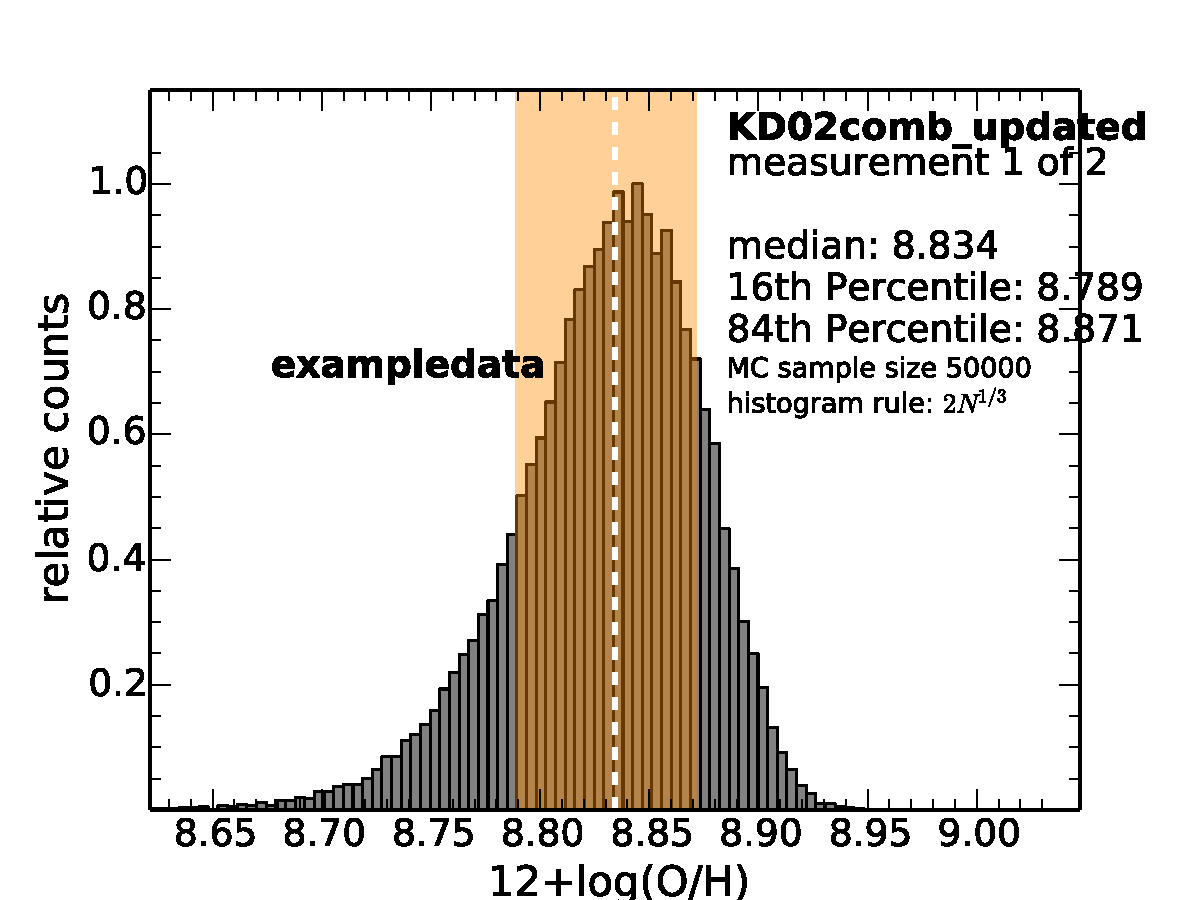
\includegraphics[width=0.95\columnwidth]{exampledata_n50000_KD02comb_updated_1.ps}
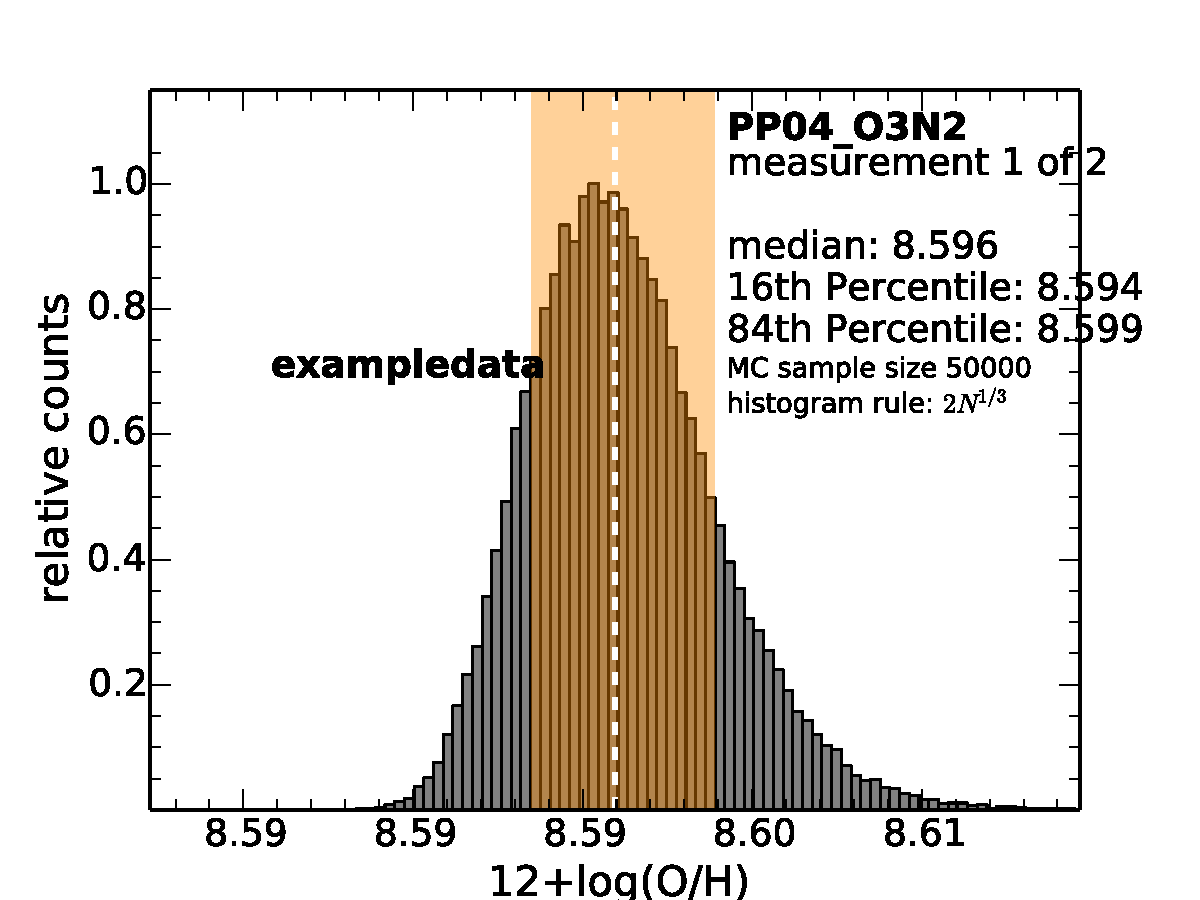
\includegraphics[width=0.95\columnwidth]{exampledata_n50000_PP04_O3N2_1.ps}
}
\vspace{0.2in}
\centerline{
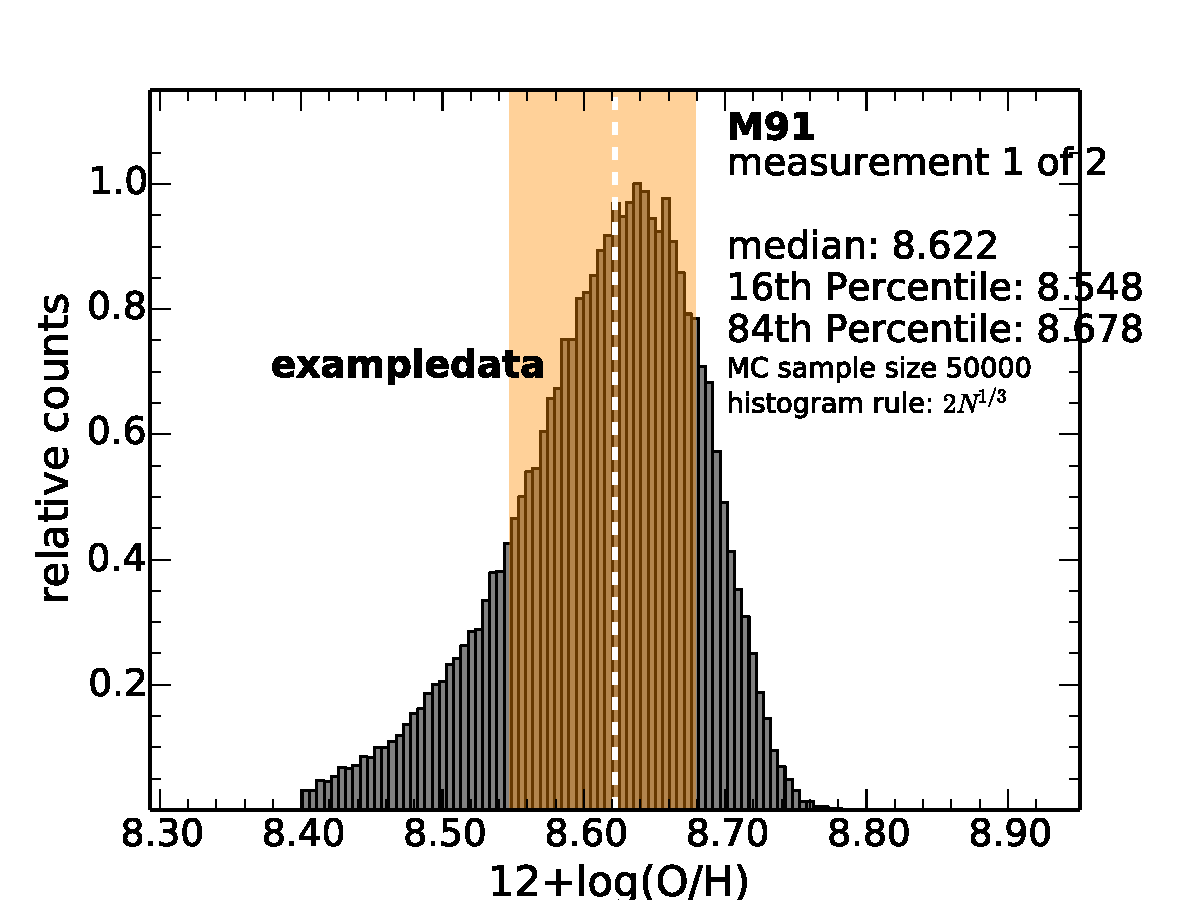
\includegraphics[width=0.95\columnwidth]{exampledata_n50000_M91_1.ps}
\includegraphics[width=0.95\columnwidth]{exampledata_n50000_E(B-V)_1.ps}
}
\caption{WILL UPDATE WITH NEW FIGURES BASED ON A PUBLISHED SN WITH SIGNFICANT E(B-V) AND WRITE MORE TEXT. Examples of confidence region determined by the algorithm, shaded in tan color.}
 \label{metallicity_distribution}
\end{center}
\vspace{-0.5in}
\end{figure*}


For computing oxygen abundances, we use the iterative code by Kewley \& Dopita (2002), which has been updated in \citet{kewley08} and reflects .. \textbf{LISA: YOUR INPUT HERE:what is the update??} which was initially written in IDL.  We translated it into python, added the new feature of obtaining uncertainties on the metallicity outputs via Monte Carlo resampling, and made it open source via github, as we explain below.

We assume that the observed emission lines to be used to indicate metallicity originate in HII regions and are not due to non-thermal excitation by e.g., AGN or interstellar shocks from SNe or stellar winds.  Tests to exclude data contaminated by such non-thermal sources have to be executed by using the recommended line ratios by e.g., \citealt{baldwin81,kauffmann03,kewley06_sdss} prior to running this code. Furthermore these lines should have all the correct calibration (at least correct relative calibration) and should have a signal-to-noise ratio (S/N) of at least 3. The latter is important for the success of the Monte Carlo resampling technique as described below.

\subsection{Input and Output of code}
Emission line flux values are fed into our Python implementation as in the original code by Kewley \& Dopita, which is written in IDL and hereafter referred to as IDL02. The inputs are emission line flux values and their uncertainties for the following lines: H$\alpha$, H$\beta$, [OI] 6300, [OII] 3727, [OIII] 4959, [OIII] 5007, [NII] 6584, [SII] 6717, [SII] 6731, SIII 9532, and SIII 9096 \textbf{CHECK!} and their uncertainties. If the fluxes for the specified lines are not available, the entry is left to 0 and the outputted oxygen abundance scales will be in only metallicity scales that use the line fluxes provided. As part of the code, the inputted line fluxes are corrected for reddening by using the observed Balmer decrement, for which H$\alpha$ and  H$\beta$ flux values are needed to be provided. We assume case B recombination and thus, the standard value of 2.86 as the
intrinsic H$\alpha$/H$\beta$ ratio \citep{osterbrock89}, and apply the standard Galactic reddening law with $R_V$ = 3.1 \citep{cardelli89}. However, the user can choose other extinction laws and $R_V$ values, if desired, given the code's open-source nature.

While other parameters, such as the ionization parameter $q$ and the electron density (using the $SiII$ lines) are computed as long as the necessary lines are provided, they are not outputted in the current version of our code $-$ however, the reader is welcome to easily modify the code to suite their needs, given it's an open-source code.

As output, we obtain metallicity values and their uncertainties in the following calibrations, as discussed in detail in \citet{kewley02,kewley08}: \citet{kewley02}(KD02, for the 4 following computations: R23, using the NIIOII ratio, using the NII/Halpha ratio, and a combined method that uses the optimal method given the input line fluxes), \citet{mcgaugh91} (M91), \citet{zaritsky94} (Z94), \citet{pilyugin01} (P01), \citet{denicolo02} (D02), 
\citet{pettini04} (2 computations: PP04-N2, PP04-O3N2) \textbf{CHECK WITH FINAL CODE}. If the line fluxes necessary for specific scales are not provided, the output  metallicities will -1    \textbf{CHECK WITH FINAL CODE}.



\subsection{Computing Uncertainties}
The novel aspect of our work is that we introduce a Monte Carlo (MC) resampling method to obtain numerous iterations via random sampling to obtain a more robust result for error estimation (e.g., \citealt{efron79,hastie09,andrae10}. Given a data set with error bars from which certain parameters are estimated, Monte Carlo resampling consists of resampling the data from its error distribution to produce alternative data sets. Here we generate a distribution of possible inputs by generating a gaussian error distribution centered on the measured line flux value, with a standard deviation corresponding to the measurement error, where we have made the assumption that the line flux error is gaussian distributed in nature\footnote{In case the user provides their own probability distribution for the emission line uncertainties (e.g. from fitting Gaussians to the emission lines via MCMC methods, the user is welcome to easily modify the code to suite their needs, given its open-source nature}. Every iteration randomly takes an input value from this distribution (for each inputted line) to run the calculations. This effectively simulates conducting multiple experiments when repeated observation is impractical or impossible, as in the case of the emission line flux data, and thus generates alternative data sets. We generated $N$ Monte Carlo samples of emission line fluxes (where an appropriate value of $N=50,000$ is determined below) and calculated the metallicity for each set of line fluxes. At the end of $N$ iterations, a parameter estimate distribution of oxygen abundance is generated for each scale by binning the results to histograms, and metallicity confidence regions are measured  (see below)\footnote{However, note this method is a conservative approach, since it overestimates the intrinsic metallicity uncertainty, as we are centering this error distribution on the measured values instead of the (unknown) true values \citep{andrae10}.} . This is done for each scale. The fiftieth (50\%) percentile, i.e.  the median, is reported as the measured value. The output of our code includes the oxygen abundance measurements plus confidence regions in all scales, as well as plots of the likelihood distributions of the oxygen abundance value in all scales. 
Figure \ref{metallicity_distribution} shows the metallicity estimate distribution for 4 representative scales - those are the same plots that are outputted as part of our code for all scales (not all shown here). As can be seen, the metallicity distributions are rarely Gaussian, for two reasons: first, since the metallicities are computed based on log values of line flux ratios, symmetric error bars in linear space will translate into asymmetric error bars in log space; and seconds, since some metallicity computations (especially those that include $R_{23}$) are non-linear since they choose an upper vs lower branch by breaking the degeneracy.

This MC resampling approach takes into account the impact of the uncertain reddening (due to the uncertainties in the measurement of the 
H$\alpha$ and H$\beta$ fluxes), when the option for de-reddened metallicities is chosen. Since for each iteration, a new reddening value is calculated based on the resampled H$\alpha$ and H$\beta$ fluxes, which is used to compute the de-reddened metallicity value, the derived distribution of metallicity values takes into account the uncertain redding. As part of the optional output, a probability distribution plot for E(B-V) is provided (see last plot in figure~\ref{metallicity_distribution}, along with confidence intervals derived using the same method as for the metallicity measurements. If either H$\alpha$ or H$\beta$ flux is not provided, then no reddening correction can be applied and the computed metallicity will not be  reddening-corrected and the E(B-V) output will be set to blank.

We note that our code  does not output the \emph{systematic} uncertainty of each scale, which are e.g., $\sim$ 0.07 dex (or 0.14 dex \textbf{CHECK}) for PP04-O2N2.  Thus systematic errors can be as large, if not larger, than the statistical errors, however, if all metallicity measurements are in the \emph{same} scale and only \emph{relative} comparisons are made, then the systematic error does not have any impact (by definition!). 

%However, the
%relative metallicity difference measured between a given pair
%of galaxies in different diagnostics is consistent with an rms
%scatter typically ?0.07 dex, and 0.15 dex between the most
%discrepant diagnostics (Kewley&Ellison 2008).


%from Kewley & Ellison08: The cause of the metallicity calibration discrepancies remains unclear. The discrepancy has been attributed to either an unknown problem with the photoionization models (Kennicutt et al. 2003) or temperature gradients or fluctuations that may cause metallicities based on the electron temperature method to underestimate the true metallicities (Stasin�ska 2002, 2005; Bresolin 2006). Until this discrepancy is resolved, the absolute metallicity scale is uncertain.

\subsubsection{Histogram Bin Size and Confidence Region}

Choosing the binning for a histogram is not trivial and \citet{hogg08} describes various data analysis recipes for selecting a histogram bin size. Too many bins will result in many empty bins and an "over-fit" histogram, while too few bins may lose features of a probability distribution. While for our default option, we use Rice Rule (e.g., \citealt{hastie09}), namely using $2* \sqrt[3]{N}$ as a number for our bins (which was appropriate for most of our test cases), we enable a number of binning options from which the user can choose, including Bayesian blocks, Knuth's rule and Doane's formula (\textbf{Fed's input here!}).

%Using a bin size of $\sqrt{N}$ was recommended, but this proved to be slightly over-fitting, and after a number of tests, we found $2* \sqrt[3]{N}$ to be appropriate for most cases.

Since the metallicity distributions are rarely Gaussian, we cannot just fit a Gaussian and report the 1-$\sigma$ intervals. In determining the confidence region intervals for asymmetric and multi-modal distributions, there are broadly three approaches (e.g., \citealt{andrae10}): choosing a symmetric interval, the shortest interval , or  a central interval.  We determined the confidence interval using the ``central" method, because it ensures that the algorithm finds the proper boundaries even in the case of multiple peaks (i.e., multimodal likelihood distributions) and for asymmetric, non-Gaussian, distributions. With the "central" method we determined the  confidence interval by choosing the left and right boundaries such that the region outside the confidence interval each equally contains $16\%$ of the total distribution for one standard deviation confidence interval - in analogy to the one-sigma-interval of the Gaussian distribution. 
 While the histograms at sufficiently high $N$, where $N$ is the total number of iterations, yielded single peaked results, at lower $N$ there were occasional multiple peaks resulting from a non-smooth gaussian being sampled. In selecting the value of $N$, we found that around $N=50,000$ provides reliably smooth histograms. 

In summary, the output for the measured value corresponds to the fiftieth (50\%) percentile, while the lower error bar corresponds to the 50$^{th}$-16$^{th}$ percentile and the upper error bar corresponds to 84$^{th}$-50$^{th}$ of the metallicity parameter estimate distribution. However, we urge that the reader always inspect the appropriate metallicity distribution plots, which are also outputted, to check for themselves whether the outputted median and confidence regions properly represent the full metallicity distribution.





\section{Comparison to prior uncertainty computation and other works }\label{comp_sec}


A previous method for determining the uncertainty in the oxygen abundance (as used in \citealt{modjaz08_Z,kewley10,rupke10,modjaz11}) was an \emph{analytic} approach of propagating the emission-line flux uncertainties: it found the maximum and minimum abundances via maximizing and minimizing, respectively, the various line ratios by adding/subtracting to the measured line values their uncertainties. For comparison we computed the metallicities and their errors in both ways (both analytic and using our current MC resampling method) for 3 representative scales. We plot our results and the residuals in Fig.\ref{comp_anal_MC}, which shows a number of important points: i) The metallicity reported as the 50th percentile of the metallicity parameter distribution from the MC resampling method is completely consistent with the analytically derived metallicity -  well within the respective error bars - and thus, the prior published results still stand. ii) The MC resampling method has smaller error bars than the analytic method, especially for the scales of M91 and KD02. This is easily understandable, since the analytic method assumes the worst-case-scenario, as it basically yields 2 metallicity parameter draws (the "minimum" and "maximum") which are in the tail of the full metallicity probability/likelihood distribution. However, the MC resampling method is the more appropriate method as it empirically characterizes the full parameter estimation distribution.
%assumes that \textbf{all} emission line measurement have been drawn from the 68\% tail of the error distribution and 

\begin{figure}[ht!]
%  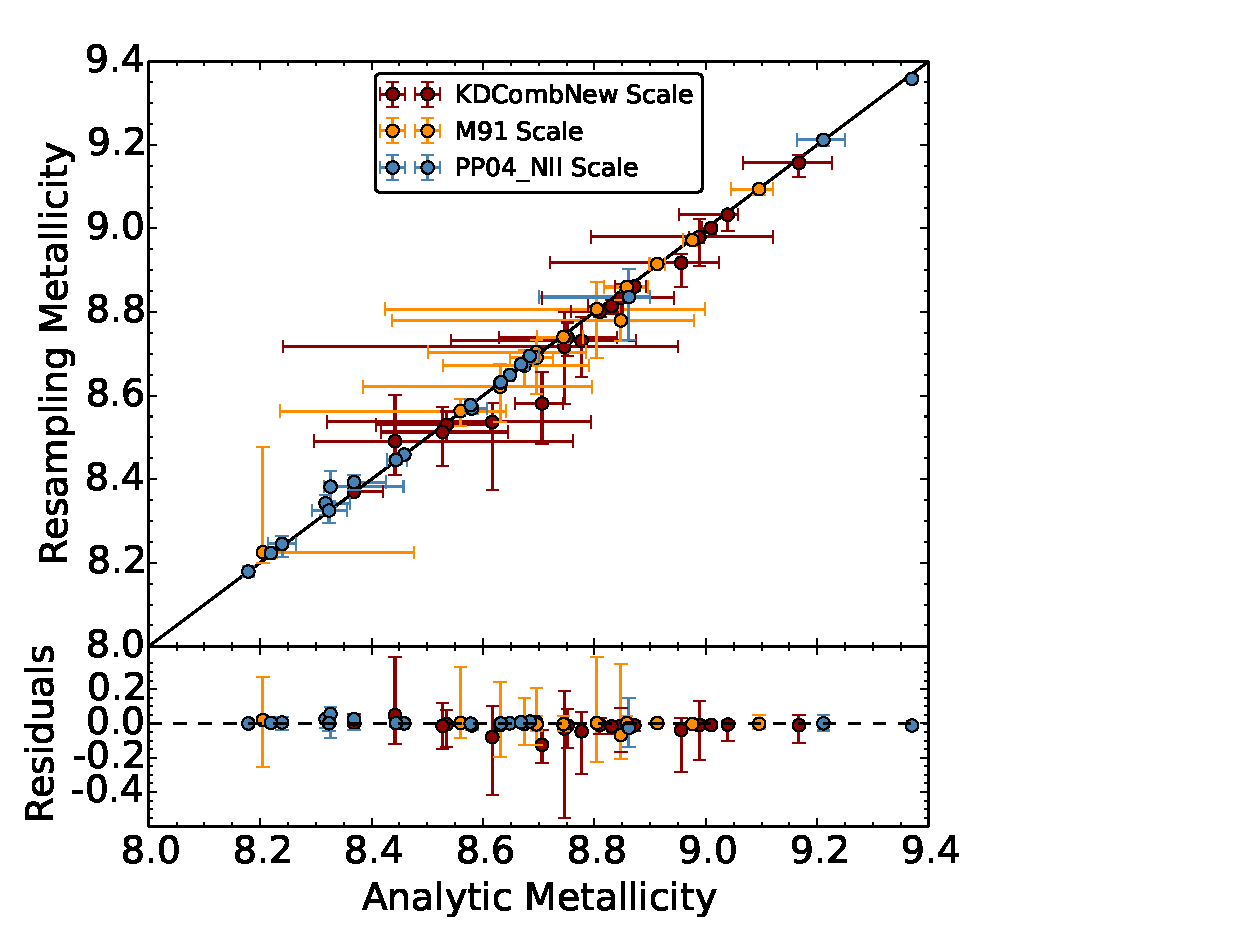
\includegraphics[trim = 10mm 0mm 10mm 0mm, clip]{abcomparison6.eps}
  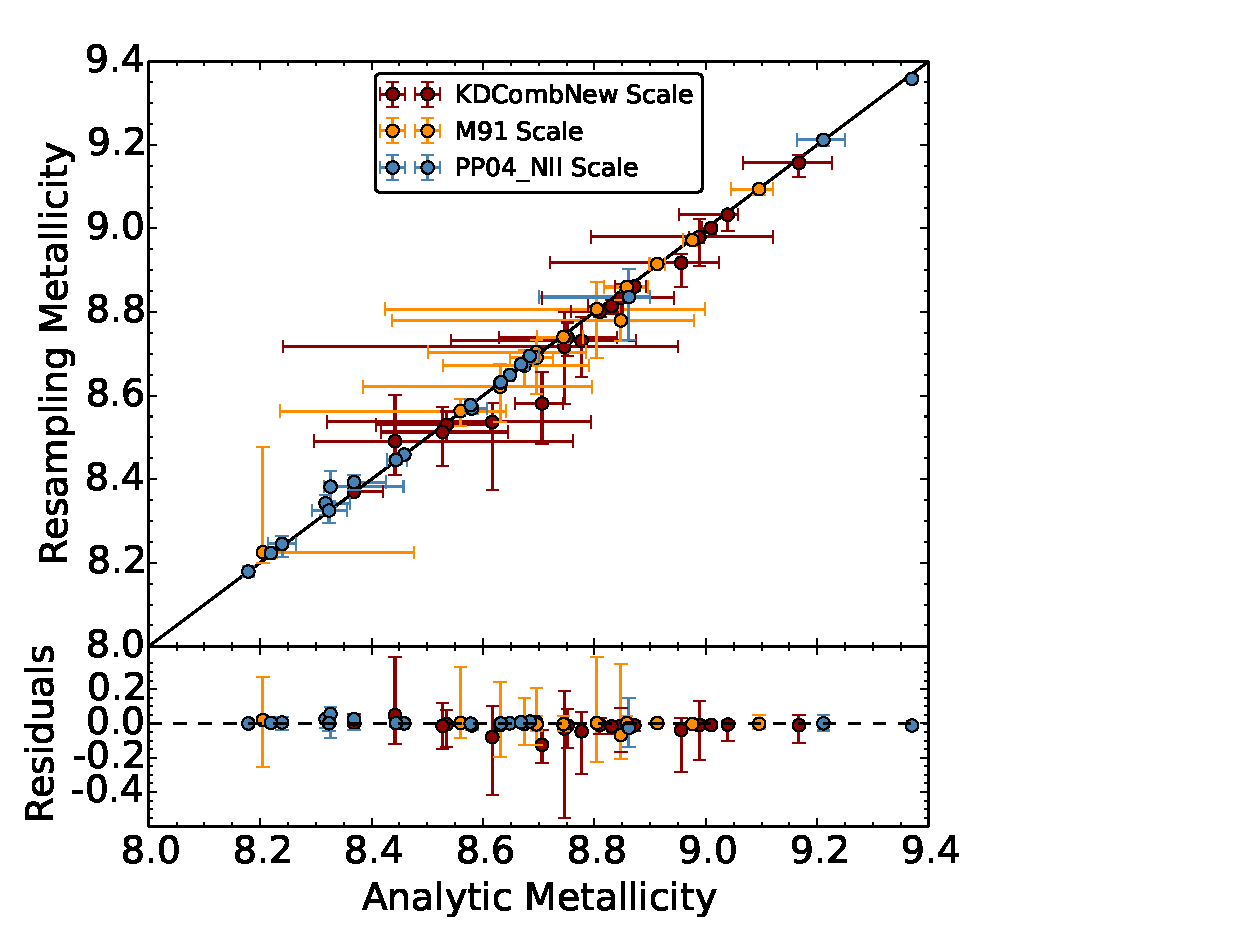
\includegraphics[width=1.2\columnwidth]{abcomparison6.eps}
   \caption{\textbf{FINISH}.Comparison of metallicity estimation between the analytic method and our Monte Carlo resampling method (top) and their residuals (bottom) for 3 different metallicity scales. Flux measurements come from 19 galaxies previously measured in \citet{modjaz11}. To add asymmetric errors in quadrature we use $residual_{min}=\sqrt {x_{max}^2 + y_{min}^2}$ and $residual_{max}=\sqrt {x_{min}^2 + y_{max}^2}$.}
 \label{comp_anal_MC}
\end{figure}

%Although the flux probability distribution function is assumed to be symmetric, the metallicity errors are asymmetric because they are derived from the log of minimized and maximized flux ratios.
%Rupke: Errors were propagated primarily using analytic expressions, but for abundance and gradient errors we employed Monte Carlo methods.

\subsection{Comparison with other works}

%Here we perform a literature review of both 


The field SN host metallicity studies has been rapidly developing as these kinds of studies may be crucial avenues for constraining the progenitor systems of different kinds of explosions- however, many of the works do not show how they compute their statistical errors (e.g., \citet{anderson10,leloudas11,sanders12,leloudas14}). While \citet{sanders12} compute the line flux errors from a Markov-Chain Monte Carlo fitting of a gaussian to the emission lines, they only mention in passing that they propagate the line flux uncertainties into the metallicity measurements, but do not describe how.

%by propagation of the uncertainties in the line flux measurements
%and the 0.07 dex diagnostic systematic error.
%( line flux errors from MCMC fitting of a gaussian to emission lines)

In contrast, the general metallicity field has considered in detail how to estimate the uncertainties in measured metallicities- however, none of those codes are open-source and many of them are for specific scales which were chosen by the authors:  \citet{moustakas10} also use MC resampling to estimate the metallicity uncertainties (in their case using 500 trials which seems to lead to a Gaussian distribution) but only do this for two scale, KK04 and \citet{pilyugin05}. For computing the metallicities of the SDSS star forming galaxies, \citet{tremonti04} fit a combination of stellar population synthesis and CLOUDY photoionization models to the observed strong emission lines [OII], Hbeta, OIII, Halpha, NII and SII and report the median of the metallicity likelihood distribution as the metallicity estimate, with the width of the distribution giving the 1 $\sigma$ (Gaussian) error. However, this is constitutes their own scale, the T04 scale.

In the last stages of preparing this manuscript \citet{blanc15} was published.  \citet{blanc15} employ Bayesian inference for doing something similar to \citet{tremonti04} - they use Bayesian inference to derive the joint and marginalized posterior probability density functions for metallicity and ionization parameter $q$ given a set of observed line fluxes and an input photoionization model. They provide a publicly available IDL implementation of their method named $IZI$ (inferring metallicities (Z) and ionization parameters) on the author's website.


\section{Conclusions}\label{comp_sec}

 \textbf{FINISH}. We hope that this open-access code will be used in many different fields where gas-phase metallicities are important, including in the emerging field of SN and GRB host galaxies, where either it is not described how they got  or no error bars are computed (e.g., \citealt{lunnan14}).

\acknowledgements
M. Modjaz is supported in parts by the NSF CAREER award AST-1352405 and by NSF award AST-1413260. 
 This research made use of NASA�s Astrophysics Data
System; the NASA/IPAC Extragalactic Database (NED), which
is operated by the Jet Propulsion Laboratory, California Institute
of Technology, under contract with the National Aeronautics
and Space Administration.



%\epsscale{1.0}
%\begin{center}
%\csvautotabular{table1.csv}
%\label{t1}
%\caption{Comparison of M-M method with MC method}
%\end{center}
%\end{figure*}



%%%%%%%%%%%%%%%%%%%%%%%%%%%%%%%%%%%%%%%%%%%
%%\clearpage
%%%%%%%%%%%%%%%% BIBLIOGRAPHY  %%%%%%%%%%%%%%%%%%%%%%%% 
\bibliographystyle{apj}
%\bibliography{refs}
\bibliography{/Users/maryammodjaz/Dropbox/refs}

\appendix

\section{Minimum Code validation}
\textbf{WORK WITH FED - and any other code specific things}
\end{document}
%,page]{appendix}
%\usepackage{amsmath}
%\usepackage{amssymb}
%\usepackage{verbatim}
%\usepackage{graphicx}
%\usepackage{epsfig}
%\usepackage{morefloats}
%\usepackage{float}
%\usepackage{lipsum}
%\usepackage{subfigure}
%\usepackage{longtable}
%\usepackage{lipsum} 
%\usepackage{rotating}
%\usepackage{wasysym}

\begin{document}
\title{Monte Carlo Method for Calculating Uncertainty in Oxygen Abundance from Strong-Line Flux Measurements}

\author{Author order to be determined: Maryam Modjaz\altaffilmark{1}, Federica Bianco\altaffilmark{1}, Seung Man Oh\altaffilmark{1,2}, David Fierroz\altaffilmark{1}, Yuqian Liu\altaffilmark{1}, Lisa Kewley\altaffilmark{3,4}}
\altaffiltext{1}{Center for Cosmology and Particle Physics, New York University, 4 Washington Place, New York, NY 10003, USA}
 \altaffiltext{2}{NYU Abu Dhabi PO Box 129188 Abu Dhabi, UAE}
 \altaffiltext{3}{Australian National University, Research School for Astronomy \& Astrophysics, Mount Stromlo Observatory, Cotter Road, Weston, ACT 2611, Australia }
 \altaffiltext{4}{ Institute of Astronomy, University of Hawaii, 2680 Woodlawn Drive, Honolulu, HI 96822, USA}
 
 
\begin{abstract}
\textbf{MODIFY \& FINALIZE AT THE END:} We present an open-source Python code for the determination of the strong-emission-line estimators of oxygen abundance in the standard scales, based on the original IDL-code in \citet{kewley02}. The standard strong line Metallicity scales and diagnostics \text{IMPROVE} have been used to estimate metal abundance by using emission line ratios. Here we introduce Monte Carlo resampling to these methods in order to better characterize an oxygen abundance confidence region.  We output probability distributions, measured values for metallicity and, when desired, for reddening E(B-V). We test our code on emission lines measurements from a sample of galaxies ($z<0.15$) and compare our metallicity results with those from previous methods. . We show that our metallicity estimate is consistent with previous methods but yields smaller uncertainties. The code is open source and can be found at www.github.com/snyugroup.
\end{abstract}
 
\section{Introduction}
The low quantity of carbon, oxygen, nitrogen, sulfur and iron among other elements provide a splash of color to the otherwise dominating greyscape of hydrogen and helium in the stars and gas of galaxies. Nevertheless, even the minute presence of heavy elements (all elements heavier than H and He, also called metals or collectively metallicity) is important for many areas of astrophysics. For example, \citet{johnson12} suggest that if it was not for the relatively high metallicity level in our solar system, planet formation may not have been possible. With $Z$ representing the mass fraction of metals, for own sun the value is measured to be  Z=0.0153 \citep{chaffau11}, though there are others who suggest a lower solar metallicity of Z=0.0134 in particular because of oxygen \citep{asplund09_rev,grevesse10}\footnote{Note that these abundances refer to the current abundances in the sun, which are lower than the value with which the sun was formed 4.56 Gyr ago, since diffusion at the bottom of the convection zone has decreased metallicity over time \citep{grevesse10}.}. Furthermore, when properly observed and estimated, metallicity measurements of the galactic gas can tightly constrain models of galaxy formation and evolution (e.g., \citealt{kewley08} and references therein), as well as shed light on the metallicity dependence and production conditions for different types of SNe and long-duration GRBs (e.g., \citealt{modjaz08_Z,levesque10_grbhosts,anderson10,modjaz11,kelly12,sanders12}).

%chaffau Z=0.0209 12+log=O/H) = 8.76�0.07 i
%Small variations in chemical abundance can often be critical indicators for stellar and galactic properties like age and activity.
%Metals are produced in the cores of stars during their fusion lifecycle but also during the extreme conditions of stellar explosions. For example, the majority of iron comes from thermonuclear explosions (SN Ia) while nearly all of oxygen is the result of core collapse (SN Ib, Ic, \& II). Since new stars are born from the clouds these explosions produce, metallicity will increase with each passing generation. Stars like our Sun, which are results of multiple generations of star formation, are often found in the more active parts of the galaxy, such as the disk, and are referred to as Population I stars. Population I stars have higher metallicity than older Population II stars, which are also present in the disk but are the exclusive members of the low activity galactic halo. Population III stars would be first generation stars with zero metallicity, but have yet to be observed.
%Besides age, metallicity also influences stellar temperature. Metals are more effective at absorbing energy coming from the interior of the star in the stellar atmosphere so their presence increases the stellar opacity. With greater absorption and opacity the radius expands to a size larger than it would be without metals and this larger size results in a cooler effective temperature. While metallicity can help indicate age or activity it's temperature and density dependencies require parameterization to properly be estimated.

However, for almost all astronomical objects, metallicity cannot be measured directly. The oxygen abundance in the gas-phase is the canonical choice of metallicity indicator for interstellar medium (ISM) studies, since oxygen is the most abundant metal and only weakly depleted onto dust grains (in contrast to refractory elements such as Mg, Si, Fe, with Fe being depleted by more than a factor of 10 in Orion; see \citealt{simondiaz11-orion}). The oxygen abundance\footnote{We note that in many cases in the literature, including here, the terms metallicity and oxygen abundance are used interchangeably.} is expressed as  $12 + \log_{10}(\frac{O}{H})$ where $O$ and $H$ are the number fractions of Oxygen and Hydrogen, respectively. Importantly, oxygen exhibits very strong nebular lines in the optical wavelength range of HII regions (e.g., \citealt{pagel79,osterbrock89,tremonti04}), and thus, many different diagnostic techniques have been developed (e.g., \citealt{kewley02,pettini04,kobulnicky04,kewley08}), which are discussed in the next section.

\subsection{The different oxygen abundance diagnostics}
The "classical" way to estimate the oxygen abundance is the electron temperature ($T_e$) method, which estimates the electron temperature and density of the nebula using a number of oxygen lines with different ionization states, including the auroral [OIII] $\lambda$4363 line, to then directly estimate the OII and OIII abundances to obtain the total oxygen abundance, after correcting for the unseen stages of ionization. However, the auroral [OIII] $\lambda$4363 line is very weak, even in low-metallicity environments, and saturates at higher metallicity (since oxygen NIR fine structure lines are cooling the nebula at higher metallicities) $-$ thus, other methods had to be developed that use other, stronger lines, in the spectra of HII regions. \textbf{MENTION DOPITA's results since the SN people are not aware of the recent developements }These are called strong-line methods and are the subject of this manuscript. Strong-line methods can be basically categorized into two types: theoretical methods, that rely on calibrating various observed line ratios using photoionization methods (basically theoretically simulating HII regions, using stellar model atmospheres, stellar populations and photoionization models) and empirical ones that calibrate various observed line ratios using observed $T_e$-based metallicities. 


For the theoretical strong-line method, one ratio that is commonly used to determine the metallicity of galaxies is ([OII] $\lambda 3727$ $+$ [OIII] $\lambda 4959,\lambda 5007$)$/$H$_\beta$ \citep{pagel79} and is referred to as R23. The drawback of this method is that it is double-valued with metallicity, and thus other line ratios need to be used to break the degeneracy between the high values ("upper branch") and the low values ("lower branch") of the R23 metallicities. Furthermore, \citet{kewley02} showed the importance of ionization parameter, which can be physically understood to correspond to the maximum velocity of an ionized front that can be driven by the local radiation field of hot massive stars that are ionizing the ISM gas. This ionization parameter needs to be taken into account in the various strong-line methods, as HII regions at the same metallicity but with different ionization parameters produce different line strengths. Calibrations of R23 by \citet{mcgaugh91} (hereafter M91) and by \citet{kewley02} (hereafter KD02) use different theoretical photoionization models and take ionization parameter into account, while other calibrations such as of \citet{zaritsky94} (hereafter Z94) do not. Thus, Z94 is mostly valid for only metal-rich galaxies.  M91 and KD02 use an iterative process to break the R23 degeneracy  (KD02 uses different ratios [NII]$/$[OII] and [NII]$/$H$_\alpha$) and to also constrain the ionization parameter $q$ in order to arrive at the metallicity estimate.

%The most direct way to estimate metallicity in spectra is to measure line fluxes absorbed or emitted by metals and non-metals. While iron lines may be present in stellar spectra, iron is less commonly found in gaseous nebulae than oxygen is. Not only is oxygen more abundant but it emits several strong lines ([OI] $\lambda 6300$, [OII] $\lambda 3727,7318,7324$, [OIII] $\lambda 4363, 4959, 5007$) visible at optical wavelengths that can also be used to quantify temperature and density. For this reason 
%While the ratio of oxygen to hydrogen line flux correlate with metallicity, the ratio of two [OIII] lines, one auroral $\lambda 4363$ and the other an excitation line at $\lambda 5007$ can be used to determine what is called the Ionization Correction Factor (ICF) (Kewley \& Dopita 2002).
As to empirical strong-line methods, the most commonly used one is that by \citet{pettini04} (hereafter PP04). PP04 used HII regions with Te-based metallicities to derive empirical fits to strong-line ratios, and introduce the line ratios of ([NII]$/$H$_\alpha$ (N2) and ([OIII]$/$H$_\beta$)$/$([NII]$/$H$_\alpha$ (O2N2) as metallicity diagnostics. Since PP04-N2 employs two closely spaced lines (Halpha and NII), which are not affected by stellar absorption, nor uncertain reddening, and are easily observed in one simple spectroscopic setup, it has become an often-used scale for at least low-z SN host galaxy studies (e.g. see metal-analysis by e.g,. \citet{sanders12,modjaz12_proc,leloudas14}. However, it is important to remember that this scale has a number of short-comings: it does not take into account the impact of ionization parameter, was initially derived based on only 137 extragalactic HII regions, and the nitrogen emission line employed saturates at high metallicity (CHECK!), and thus this method may not be well-suited for high-metallicity galaxies. An updated calibration by \citet{marino13} based on many more Te-based metallicities (almost three time larger that that of PP04) derives a significantly shallower slope between O3N2 index and oxygen abundance than the PP04 calibration.


As can be seen, each scale has different advantages and disadvantages and may be used in different metallicity regimes (see detailed discussion in e.g.,  \citealt{kewley02,stasinska02,kewley08,moustakas10,dopita13,blanc15}). Thus, this open-source code outputs the oxygen abundance in the main 6 metallicity scales (for which the KD02 diagnostic has four outputs and the PP04 diagnostic has two outputs). While there is a long-standing debate about which diagnostic to use, as there are systematic metallicity offsets between different methods (recombination lines vs.  strong-line method vs. "direct" $T_e$ method, see the above sources), \emph{the relative metallicity trends can be considered robust, if the analysis is performed self-consistently in the same scale, and trends are seen across different scales \citep{kewley08,moustakas10}}. Note however, that while there are conversion values between different scales \citep{kewley08}, they apply for large data sets, since those conversion values were derived based on ten thousands of SDSS galaxies, and thus should be used with caution (or not at all) for smaller samples. In addition, there the debate about the value of the solar oxygen abundance value \citep{asplund09_rev,chaffau11}, such that the absolute oxygen calibration is still uncertain.




Here we introduce the open-source code "". pro .. In \S~\ref{method_sec} we describe our method, the input and output values of the code. In \S~\ref{comp_sec}, we compare our method of obtaining abundance uncertainties to previous methods in the literature. 
%\begin{figure}[H]
%\epsscale{1.0} 
%\begin{center}
%\includegraphics[width=0.89\columnwidth]{fig1.png} 
%\caption{Example of a sampled Gaussian. 50,000 points from a Gaussian distribution were selected in this case}
%\label{f1}
%\end{center}
%\end{figure}


\section{Description of Metallicity code}\label{method_sec}


\begin{figure*}[!HT]
%\epsscale{0.6}
\begin{center}
\centerline{
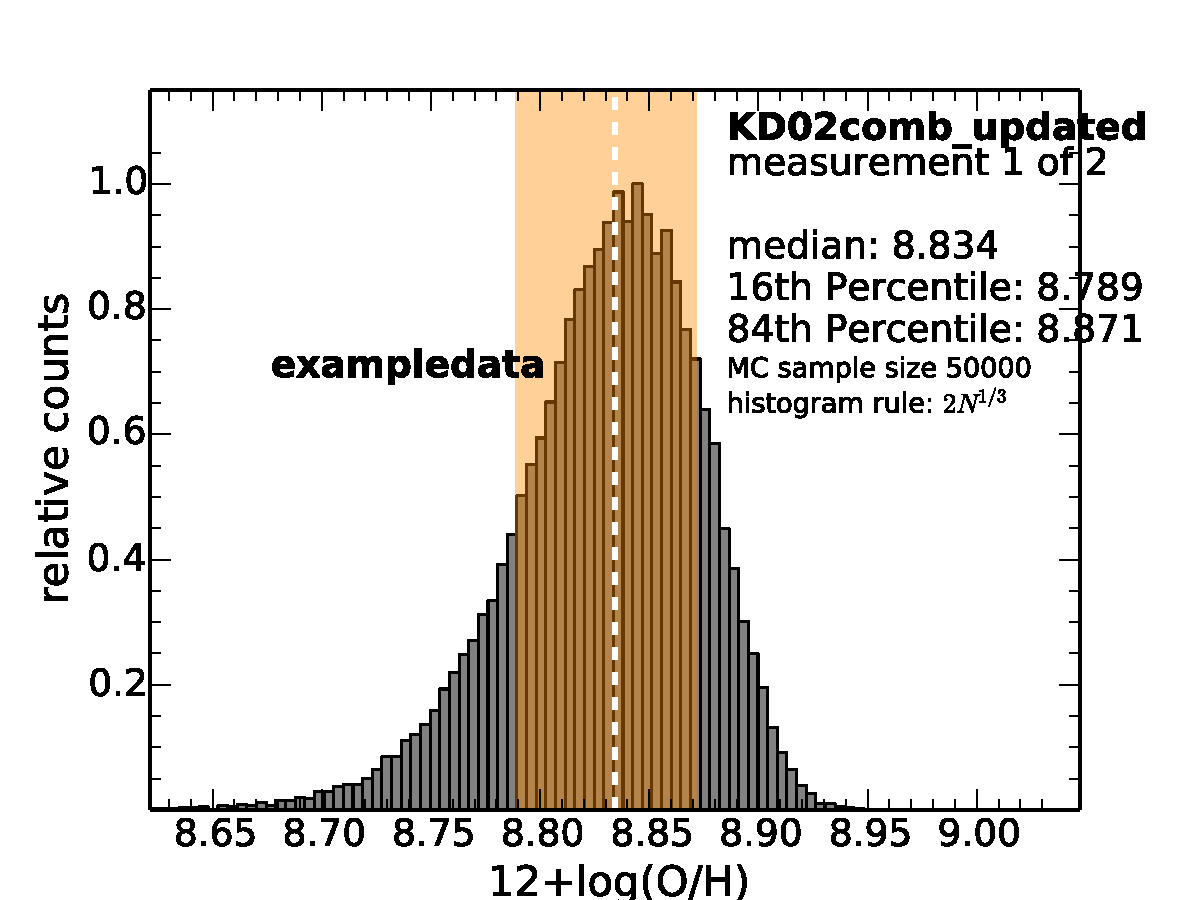
\includegraphics[width=0.95\columnwidth]{exampledata_n50000_KD02comb_updated_1.ps}
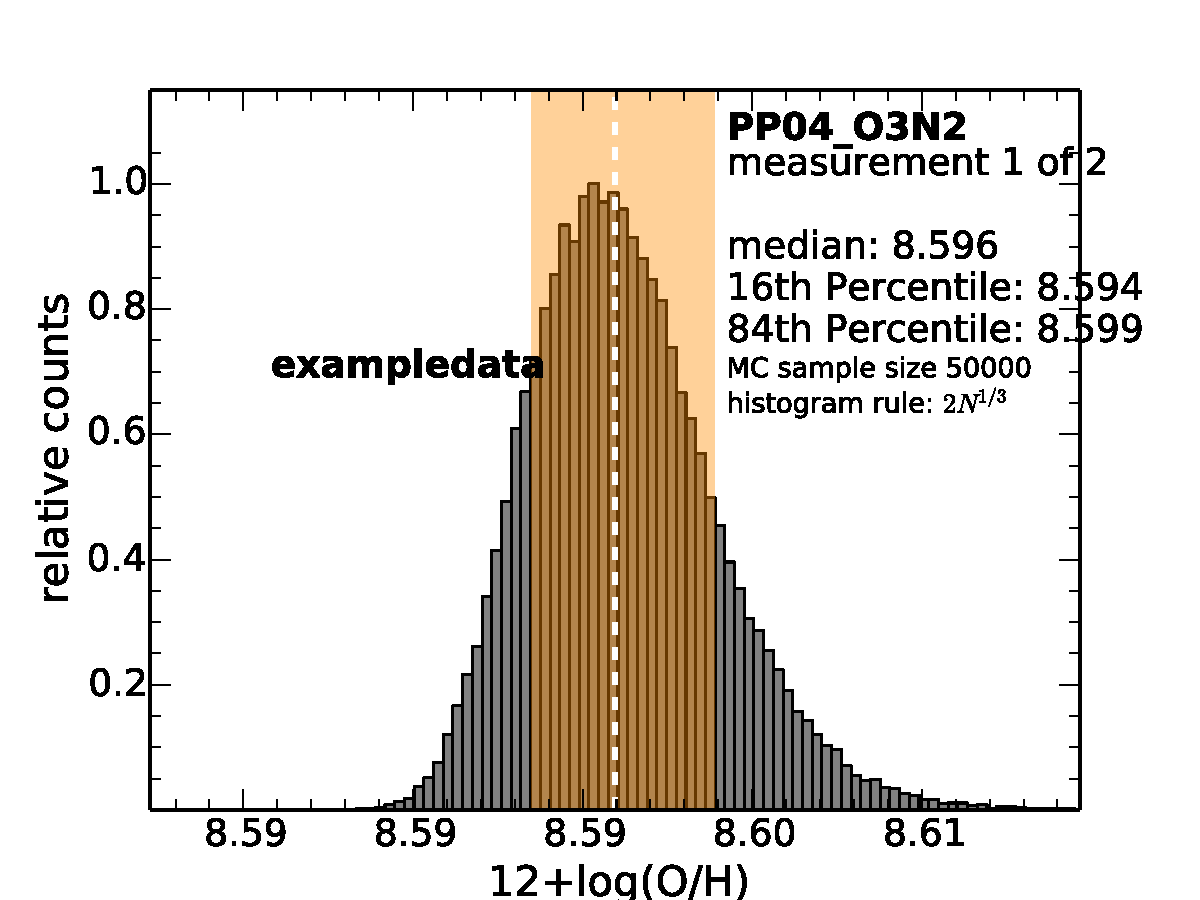
\includegraphics[width=0.95\columnwidth]{exampledata_n50000_PP04_O3N2_1.ps}
}
\vspace{0.2in}
\centerline{
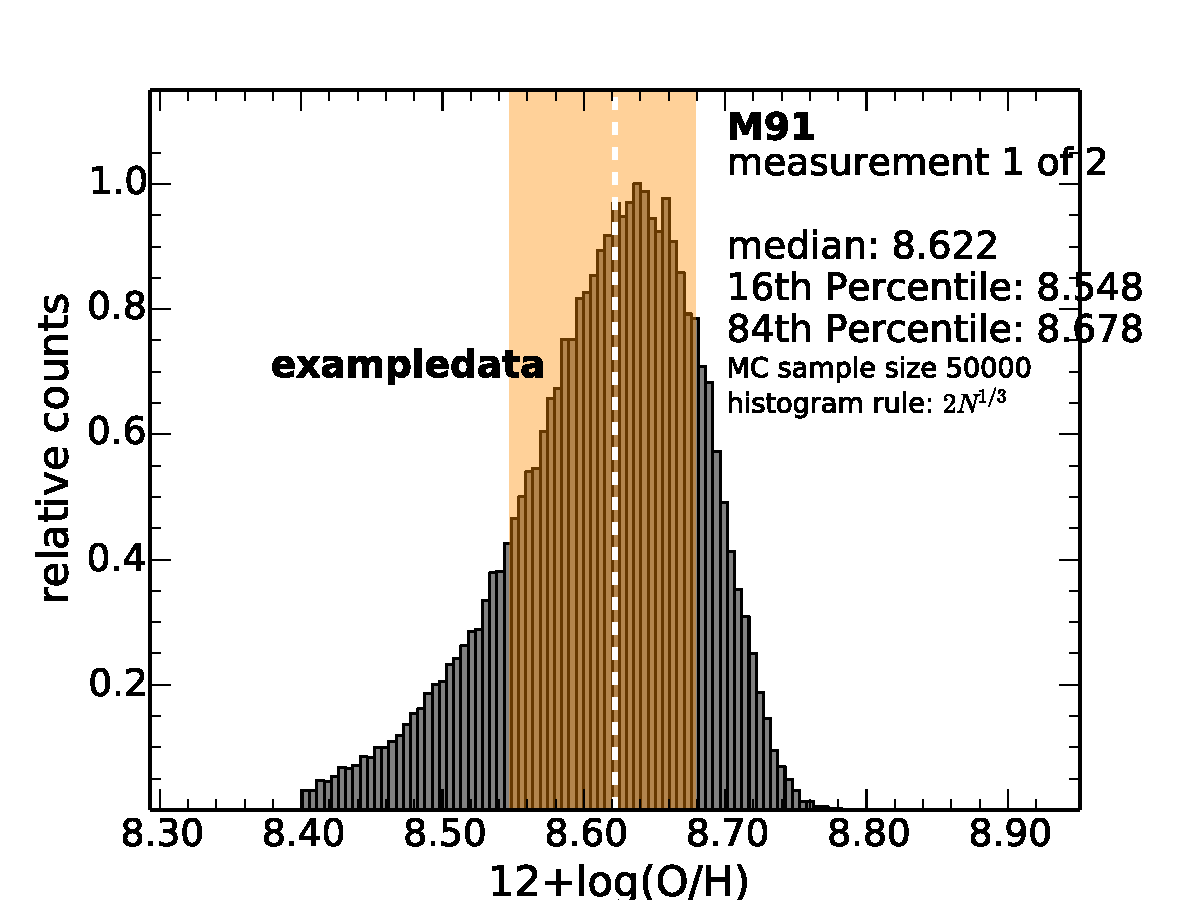
\includegraphics[width=0.95\columnwidth]{exampledata_n50000_M91_1.ps}
\includegraphics[width=0.95\columnwidth]{exampledata_n50000_E(B-V)_1.ps}
}
\caption{WILL UPDATE WITH NEW FIGURES BASED ON A PUBLISHED SN WITH SIGNFICANT E(B-V) AND WRITE MORE TEXT. Examples of confidence region determined by the algorithm, shaded in tan color.}
 \label{metallicity_distribution}
\end{center}
\vspace{-0.5in}
\end{figure*}


For computing oxygen abundances, we use the iterative code by Kewley \& Dopita (2002), which has been updated in \citet{kewley08} and reflects .. \textbf{LISA: YOUR INPUT HERE:what is the update??} which was initially written in IDL.  We translated it into python, added the new feature of obtaining uncertainties on the metallicity outputs via Monte Carlo resampling, and made it open source via github, as we explain below.

We assume that the observed emission lines to be used to indicate metallicity originate in HII regions and are not due to non-thermal excitation by e.g., AGN or interstellar shocks from SNe or stellar winds.  Tests to exclude data contaminated by such non-thermal sources have to be executed by using the recommended line ratios by e.g., \citealt{baldwin81,kauffmann03,kewley06_sdss} prior to running this code. Furthermore these lines should have all the correct calibration (at least correct relative calibration) and should have a signal-to-noise ratio (S/N) of at least 3. The latter is important for the success of the Monte Carlo resampling technique as described below.

\subsection{Input and Output of code}
Emission line flux values are fed into our Python implementation as in the original code by Kewley \& Dopita, which is written in IDL and hereafter referred to as IDL02. The inputs are emission line flux values and their uncertainties for the following lines: H$\alpha$, H$\beta$, [OI] 6300, [OII] 3727, [OIII] 4959, [OIII] 5007, [NII] 6584, [SII] 6717, [SII] 6731, SIII 9532, and SIII 9096 \textbf{CHECK!} and their uncertainties. If the fluxes for the specified lines are not available, the entry is left to 0 and the outputted oxygen abundance scales will be in only metallicity scales that use the line fluxes provided. As part of the code, the inputted line fluxes are corrected for reddening by using the observed Balmer decrement, for which H$\alpha$ and  H$\beta$ flux values are needed to be provided. We assume case B recombination and thus, the standard value of 2.86 as the
intrinsic H$\alpha$/H$\beta$ ratio \citep{osterbrock89}, and apply the standard Galactic reddening law with $R_V$ = 3.1 \citep{cardelli89}. However, the user can choose other extinction laws and $R_V$ values, if desired, given the code's open-source nature.

While other parameters, such as the ionization parameter $q$ and the electron density (using the $SiII$ lines) are computed as long as the necessary lines are provided, they are not outputted in the current version of our code $-$ however, the reader is welcome to easily modify the code to suite their needs, given it's an open-source code.

As output, we obtain metallicity values and their uncertainties in the following calibrations, as discussed in detail in \citet{kewley02,kewley08}: \citet{kewley02}(KD02, for the 4 following computations: R23, using the NIIOII ratio, using the NII/Halpha ratio, and a combined method that uses the optimal method given the input line fluxes), \citet{mcgaugh91} (M91), \citet{zaritsky94} (Z94), \citet{pilyugin01} (P01), \citet{denicolo02} (D02), 
\citet{pettini04} (2 computations: PP04-N2, PP04-O3N2) \textbf{CHECK WITH FINAL CODE}. If the line fluxes necessary for specific scales are not provided, the output  metallicities will -1    \textbf{CHECK WITH FINAL CODE}.



\subsection{Computing Uncertainties}
The novel aspect of our work is that we introduce a Monte Carlo (MC) resampling method to obtain numerous iterations via random sampling to obtain a more robust result for error estimation (e.g., \citealt{efron79,hastie09,andrae10}. Given a data set with error bars from which certain parameters are estimated, Monte Carlo resampling consists of resampling the data from its error distribution to produce alternative data sets. Here we generate a distribution of possible inputs by generating a gaussian error distribution centered on the measured line flux value, with a standard deviation corresponding to the measurement error, where we have made the assumption that the line flux error is gaussian distributed in nature\footnote{In case the user provides their own probability distribution for the emission line uncertainties (e.g. from fitting Gaussians to the emission lines via MCMC methods, the user is welcome to easily modify the code to suite their needs, given its open-source nature}. Every iteration randomly takes an input value from this distribution (for each inputted line) to run the calculations. This effectively simulates conducting multiple experiments when repeated observation is impractical or impossible, as in the case of the emission line flux data, and thus generates alternative data sets. We generated $N$ Monte Carlo samples of emission line fluxes (where an appropriate value of $N=50,000$ is determined below) and calculated the metallicity for each set of line fluxes. At the end of $N$ iterations, a parameter estimate distribution of oxygen abundance is generated for each scale by binning the results to histograms, and metallicity confidence regions are measured  (see below)\footnote{However, note this method is a conservative approach, since it overestimates the intrinsic metallicity uncertainty, as we are centering this error distribution on the measured values instead of the (unknown) true values \citep{andrae10}.} . This is done for each scale. The fiftieth (50\%) percentile, i.e.  the median, is reported as the measured value. The output of our code includes the oxygen abundance measurements plus confidence regions in all scales, as well as plots of the likelihood distributions of the oxygen abundance value in all scales. 
Figure \ref{metallicity_distribution} shows the metallicity estimate distribution for 4 representative scales - those are the same plots that are outputted as part of our code for all scales (not all shown here). As can be seen, the metallicity distributions are rarely Gaussian, for two reasons: first, since the metallicities are computed based on log values of line flux ratios, symmetric error bars in linear space will translate into asymmetric error bars in log space; and seconds, since some metallicity computations (especially those that include $R_{23}$) are non-linear since they choose an upper vs lower branch by breaking the degeneracy.

This MC resampling approach takes into account the impact of the uncertain reddening (due to the uncertainties in the measurement of the 
H$\alpha$ and H$\beta$ fluxes), when the option for de-reddened metallicities is chosen. Since for each iteration, a new reddening value is calculated based on the resampled H$\alpha$ and H$\beta$ fluxes, which is used to compute the de-reddened metallicity value, the derived distribution of metallicity values takes into account the uncertain redding. As part of the optional output, a probability distribution plot for E(B-V) is provided (see last plot in figure~\ref{metallicity_distribution}, along with confidence intervals derived using the same method as for the metallicity measurements. If either H$\alpha$ or H$\beta$ flux is not provided, then no reddening correction can be applied and the computed metallicity will not be  reddening-corrected and the E(B-V) output will be set to blank.

We note that our code  does not output the \emph{systematic} uncertainty of each scale, which are e.g., $\sim$ 0.07 dex (or 0.14 dex \textbf{CHECK}) for PP04-O2N2.  Thus systematic errors can be as large, if not larger, than the statistical errors, however, if all metallicity measurements are in the \emph{same} scale and only \emph{relative} comparisons are made, then the systematic error does not have any impact (by definition!). 

%However, the
%relative metallicity difference measured between a given pair
%of galaxies in different diagnostics is consistent with an rms
%scatter typically ?0.07 dex, and 0.15 dex between the most
%discrepant diagnostics (Kewley&Ellison 2008).


%from Kewley & Ellison08: The cause of the metallicity calibration discrepancies remains unclear. The discrepancy has been attributed to either an unknown problem with the photoionization models (Kennicutt et al. 2003) or temperature gradients or fluctuations that may cause metallicities based on the electron temperature method to underestimate the true metallicities (Stasin�ska 2002, 2005; Bresolin 2006). Until this discrepancy is resolved, the absolute metallicity scale is uncertain.

\subsubsection{Histogram Bin Size and Confidence Region}

Choosing the binning for a histogram is not trivial and \citet{hogg08} describes various data analysis recipes for selecting a histogram bin size. Too many bins will result in many empty bins and an "over-fit" histogram, while too few bins may lose features of a probability distribution. While for our default option, we use Rice Rule (e.g., \citealt{hastie09}), namely using $2* \sqrt[3]{N}$ as a number for our bins (which was appropriate for most of our test cases), we enable a number of binning options from which the user can choose, including Bayesian blocks, Knuth's rule and Doane's formula (\textbf{Fed's input here!}).

%Using a bin size of $\sqrt{N}$ was recommended, but this proved to be slightly over-fitting, and after a number of tests, we found $2* \sqrt[3]{N}$ to be appropriate for most cases.

Since the metallicity distributions are rarely Gaussian, we cannot just fit a Gaussian and report the 1-$\sigma$ intervals. In determining the confidence region intervals for asymmetric and multi-modal distributions, there are broadly three approaches (e.g., \citealt{andrae10}): choosing a symmetric interval, the shortest interval , or  a central interval.  We determined the confidence interval using the ``central" method, because it ensures that the algorithm finds the proper boundaries even in the case of multiple peaks (i.e., multimodal likelihood distributions) and for asymmetric, non-Gaussian, distributions. With the "central" method we determined the  confidence interval by choosing the left and right boundaries such that the region outside the confidence interval each equally contains $16\%$ of the total distribution for one standard deviation confidence interval - in analogy to the one-sigma-interval of the Gaussian distribution. 
 While the histograms at sufficiently high $N$, where $N$ is the total number of iterations, yielded single peaked results, at lower $N$ there were occasional multiple peaks resulting from a non-smooth gaussian being sampled. In selecting the value of $N$, we found that around $N=50,000$ provides reliably smooth histograms. 

In summary, the output for the measured value corresponds to the fiftieth (50\%) percentile, while the lower error bar corresponds to the 50$^{th}$-16$^{th}$ percentile and the upper error bar corresponds to 84$^{th}$-50$^{th}$ of the metallicity parameter estimate distribution. However, we urge that the reader always inspect the appropriate metallicity distribution plots, which are also outputted, to check for themselves whether the outputted median and confidence regions properly represent the full metallicity distribution.





\section{Comparison to prior uncertainty computation and other works }\label{comp_sec}


A previous method for determining the uncertainty in the oxygen abundance (as used in \citealt{modjaz08_Z,kewley10,rupke10,modjaz11}) was an \emph{analytic} approach of propagating the emission-line flux uncertainties: it found the maximum and minimum abundances via maximizing and minimizing, respectively, the various line ratios by adding/subtracting to the measured line values their uncertainties. For comparison we computed the metallicities and their errors in both ways (both analytic and using our current MC resampling method) for 3 representative scales. We plot our results and the residuals in Fig.\ref{comp_anal_MC}, which shows a number of important points: i) The metallicity reported as the 50th percentile of the metallicity parameter distribution from the MC resampling method is completely consistent with the analytically derived metallicity -  well within the respective error bars - and thus, the prior published results still stand. ii) The MC resampling method has smaller error bars than the analytic method, especially for the scales of M91 and KD02. This is easily understandable, since the analytic method assumes the worst-case-scenario, as it basically yields 2 metallicity parameter draws (the "minimum" and "maximum") which are in the tail of the full metallicity probability/likelihood distribution. However, the MC resampling method is the more appropriate method as it empirically characterizes the full parameter estimation distribution.
%assumes that \textbf{all} emission line measurement have been drawn from the 68\% tail of the error distribution and 

\begin{figure}[ht!]
%  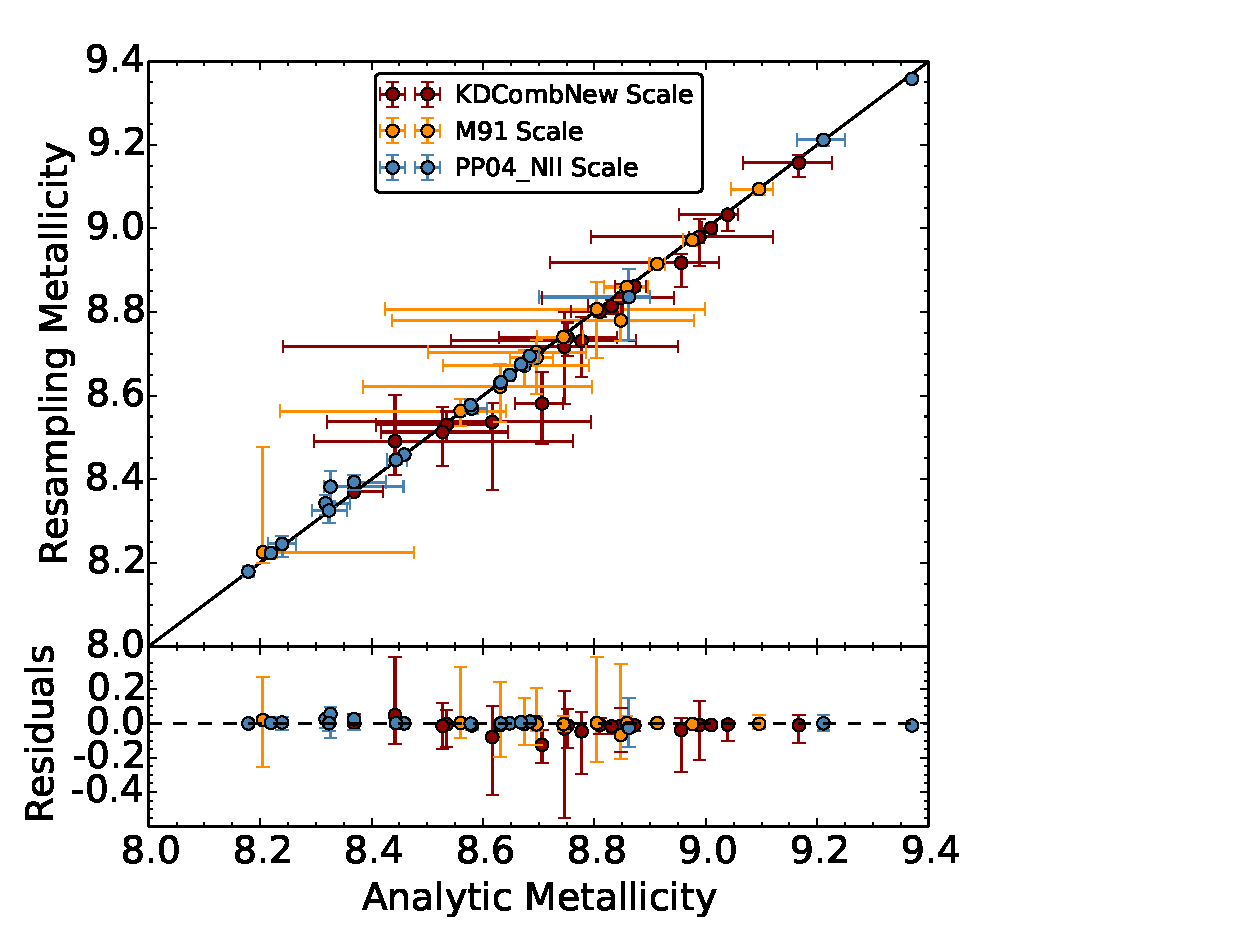
\includegraphics[trim = 10mm 0mm 10mm 0mm, clip]{abcomparison6.eps}
  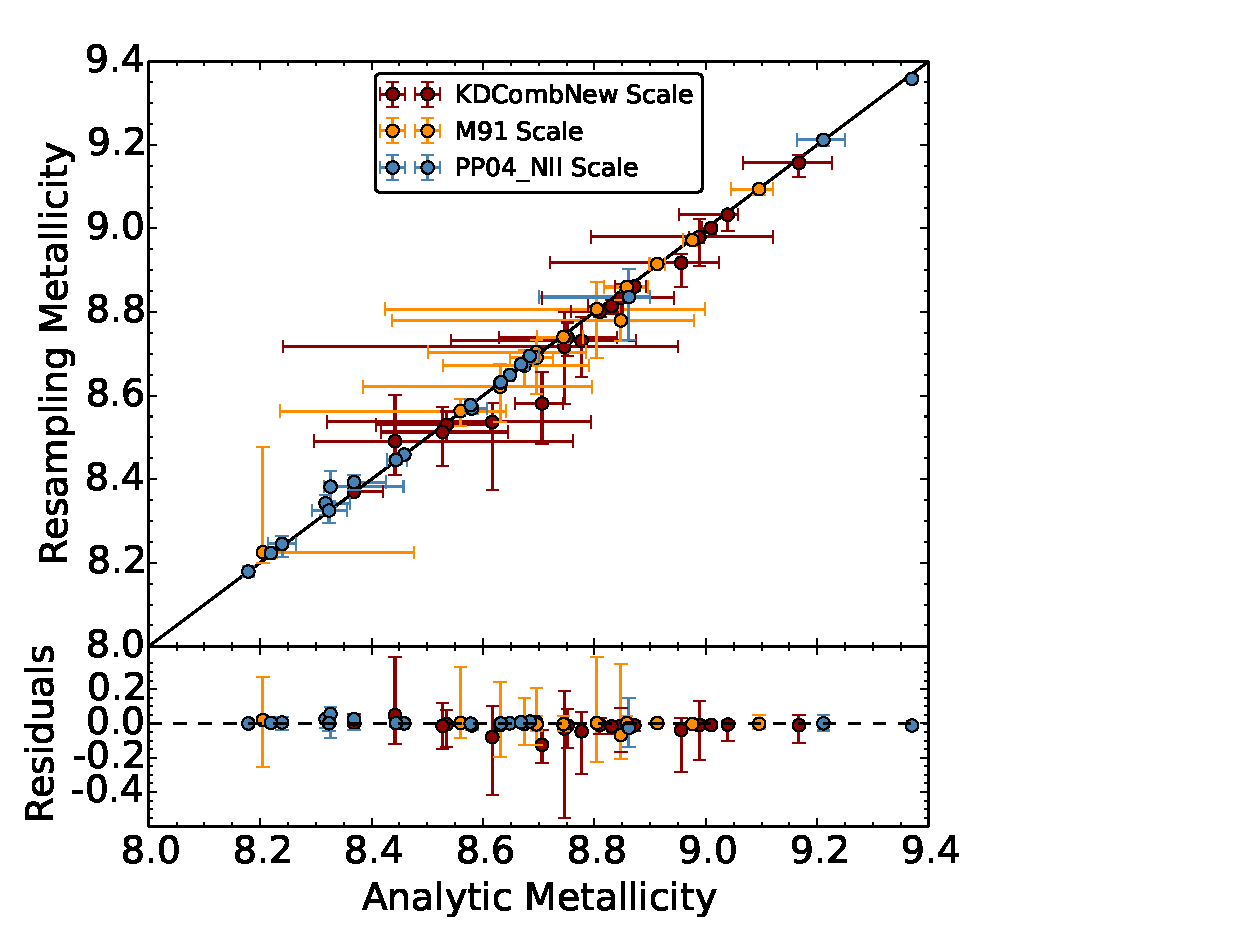
\includegraphics[width=1.2\columnwidth]{abcomparison6.eps}
   \caption{\textbf{FINISH}.Comparison of metallicity estimation between the analytic method and our Monte Carlo resampling method (top) and their residuals (bottom) for 3 different metallicity scales. Flux measurements come from 19 galaxies previously measured in \citet{modjaz11}. To add asymmetric errors in quadrature we use $residual_{min}=\sqrt {x_{max}^2 + y_{min}^2}$ and $residual_{max}=\sqrt {x_{min}^2 + y_{max}^2}$.}
 \label{comp_anal_MC}
\end{figure}

%Although the flux probability distribution function is assumed to be symmetric, the metallicity errors are asymmetric because they are derived from the log of minimized and maximized flux ratios.
%Rupke: Errors were propagated primarily using analytic expressions, but for abundance and gradient errors we employed Monte Carlo methods.

\subsection{Comparison with other works}

%Here we perform a literature review of both 


The field SN host metallicity studies has been rapidly developing as these kinds of studies may be crucial avenues for constraining the progenitor systems of different kinds of explosions- however, many of the works do not show how they compute their statistical errors (e.g., \citet{anderson10,leloudas11,sanders12,leloudas14}). While \citet{sanders12} compute the line flux errors from a Markov-Chain Monte Carlo fitting of a gaussian to the emission lines, they only mention in passing that they propagate the line flux uncertainties into the metallicity measurements, but do not describe how.

%by propagation of the uncertainties in the line flux measurements
%and the 0.07 dex diagnostic systematic error.
%( line flux errors from MCMC fitting of a gaussian to emission lines)

In contrast, the general metallicity field has considered in detail how to estimate the uncertainties in measured metallicities- however, none of those codes are open-source and many of them are for specific scales which were chosen by the authors:  \citet{moustakas10} also use MC resampling to estimate the metallicity uncertainties (in their case using 500 trials which seems to lead to a Gaussian distribution) but only do this for two scale, KK04 and \citet{pilyugin05}. For computing the metallicities of the SDSS star forming galaxies, \citet{tremonti04} fit a combination of stellar population synthesis and CLOUDY photoionization models to the observed strong emission lines [OII], Hbeta, OIII, Halpha, NII and SII and report the median of the metallicity likelihood distribution as the metallicity estimate, with the width of the distribution giving the 1 $\sigma$ (Gaussian) error. However, this is constitutes their own scale, the T04 scale.

In the last stages of preparing this manuscript \citet{blanc15} was published.  \citet{blanc15} employ Bayesian inference for doing something similar to \citet{tremonti04} - they use Bayesian inference to derive the joint and marginalized posterior probability density functions for metallicity and ionization parameter $q$ given a set of observed line fluxes and an input photoionization model. They provide a publicly available IDL implementation of their method named $IZI$ (inferring metallicities (Z) and ionization parameters) on the author's website.


\section{Conclusions}\label{comp_sec}

 \textbf{FINISH}. We hope that this open-access code will be used in many different fields where gas-phase metallicities are important, including in the emerging field of SN and GRB host galaxies, where either it is not described how they got  or no error bars are computed (e.g., \citealt{lunnan14}).

\acknowledgements
M. Modjaz is supported in parts by the NSF CAREER award AST-1352405 and by NSF award AST-1413260. 
 This research made use of NASA�s Astrophysics Data
System; the NASA/IPAC Extragalactic Database (NED), which
is operated by the Jet Propulsion Laboratory, California Institute
of Technology, under contract with the National Aeronautics
and Space Administration.



%\epsscale{1.0}
%\begin{center}
%\csvautotabular{table1.csv}
%\label{t1}
%\caption{Comparison of M-M method with MC method}
%\end{center}
%\end{figure*}



%%%%%%%%%%%%%%%%%%%%%%%%%%%%%%%%%%%%%%%%%%%
%%\clearpage
%%%%%%%%%%%%%%%% BIBLIOGRAPHY  %%%%%%%%%%%%%%%%%%%%%%%% 
\bibliographystyle{apj}
%\bibliography{refs}
\bibliography{/Users/maryammodjaz/Dropbox/refs}

\appendix

\section{Minimum Code validation}
\textbf{WORK WITH FED - and any other code specific things}
\end{document}
%,page]{appendix}
%\usepackage{amsmath}
%\usepackage{amssymb}
%\usepackage{verbatim}
%\usepackage{graphicx}
%\usepackage{epsfig}
%\usepackage{morefloats}
%\usepackage{float}
%\usepackage{lipsum}
%\usepackage{subfigure}
%\usepackage{longtable}
%\usepackage{lipsum} 
%\usepackage{rotating}
%\usepackage{wasysym}

\begin{document}
\title{Monte Carlo Method for Calculating Uncertainty in Oxygen Abundance from Strong-Line Flux Measurements}

\author{Author order to be determined: Maryam Modjaz\altaffilmark{1}, Federica Bianco\altaffilmark{1}, Seung Man Oh\altaffilmark{1,2}, David Fierroz\altaffilmark{1}, Yuqian Liu\altaffilmark{1}, Lisa Kewley\altaffilmark{3,4}}
\altaffiltext{1}{Center for Cosmology and Particle Physics, New York University, 4 Washington Place, New York, NY 10003, USA}
 \altaffiltext{2}{NYU Abu Dhabi PO Box 129188 Abu Dhabi, UAE}
 \altaffiltext{3}{Australian National University, Research School for Astronomy \& Astrophysics, Mount Stromlo Observatory, Cotter Road, Weston, ACT 2611, Australia }
 \altaffiltext{4}{ Institute of Astronomy, University of Hawaii, 2680 Woodlawn Drive, Honolulu, HI 96822, USA}
 
 
\begin{abstract}
\textbf{MODIFY \& FINALIZE AT THE END:} We present an open-source Python code for the determination of the strong-emission-line estimators of oxygen abundance in the standard scales, based on the original IDL-code in \citet{kewley02}. The standard strong line Metallicity scales and diagnostics \text{IMPROVE} have been used to estimate metal abundance by using emission line ratios. Here we introduce Monte Carlo resampling to these methods in order to better characterize an oxygen abundance confidence region.  We output probability distributions, measured values for metallicity and, when desired, for reddening E(B-V). We test our code on emission lines measurements from a sample of galaxies ($z<0.15$) and compare our metallicity results with those from previous methods. . We show that our metallicity estimate is consistent with previous methods but yields smaller uncertainties. The code is open source and can be found at www.github.com/snyugroup.
\end{abstract}
 
\section{Introduction}
The low quantity of carbon, oxygen, nitrogen, sulfur and iron among other elements provide a splash of color to the otherwise dominating greyscape of hydrogen and helium in the stars and gas of galaxies. Nevertheless, even the minute presence of heavy elements (all elements heavier than H and He, also called metals or collectively metallicity) is important for many areas of astrophysics. For example, \citet{johnson12} suggest that if it was not for the relatively high metallicity level in our solar system, planet formation may not have been possible. With $Z$ representing the mass fraction of metals, for own sun the value is measured to be  Z=0.0153 \citep{chaffau11}, though there are others who suggest a lower solar metallicity of Z=0.0134 in particular because of oxygen \citep{asplund09_rev,grevesse10}\footnote{Note that these abundances refer to the current abundances in the sun, which are lower than the value with which the sun was formed 4.56 Gyr ago, since diffusion at the bottom of the convection zone has decreased metallicity over time \citep{grevesse10}.}. Furthermore, when properly observed and estimated, metallicity measurements of the galactic gas can tightly constrain models of galaxy formation and evolution (e.g., \citealt{kewley08} and references therein), as well as shed light on the metallicity dependence and production conditions for different types of SNe and long-duration GRBs (e.g., \citealt{modjaz08_Z,levesque10_grbhosts,anderson10,modjaz11,kelly12,sanders12}).

%chaffau Z=0.0209 12+log=O/H) = 8.76�0.07 i
%Small variations in chemical abundance can often be critical indicators for stellar and galactic properties like age and activity.
%Metals are produced in the cores of stars during their fusion lifecycle but also during the extreme conditions of stellar explosions. For example, the majority of iron comes from thermonuclear explosions (SN Ia) while nearly all of oxygen is the result of core collapse (SN Ib, Ic, \& II). Since new stars are born from the clouds these explosions produce, metallicity will increase with each passing generation. Stars like our Sun, which are results of multiple generations of star formation, are often found in the more active parts of the galaxy, such as the disk, and are referred to as Population I stars. Population I stars have higher metallicity than older Population II stars, which are also present in the disk but are the exclusive members of the low activity galactic halo. Population III stars would be first generation stars with zero metallicity, but have yet to be observed.
%Besides age, metallicity also influences stellar temperature. Metals are more effective at absorbing energy coming from the interior of the star in the stellar atmosphere so their presence increases the stellar opacity. With greater absorption and opacity the radius expands to a size larger than it would be without metals and this larger size results in a cooler effective temperature. While metallicity can help indicate age or activity it's temperature and density dependencies require parameterization to properly be estimated.

However, for almost all astronomical objects, metallicity cannot be measured directly. The oxygen abundance in the gas-phase is the canonical choice of metallicity indicator for interstellar medium (ISM) studies, since oxygen is the most abundant metal and only weakly depleted onto dust grains (in contrast to refractory elements such as Mg, Si, Fe, with Fe being depleted by more than a factor of 10 in Orion; see \citealt{simondiaz11-orion}). The oxygen abundance\footnote{We note that in many cases in the literature, including here, the terms metallicity and oxygen abundance are used interchangeably.} is expressed as  $12 + \log_{10}(\frac{O}{H})$ where $O$ and $H$ are the number fractions of Oxygen and Hydrogen, respectively. Importantly, oxygen exhibits very strong nebular lines in the optical wavelength range of HII regions (e.g., \citealt{pagel79,osterbrock89,tremonti04}), and thus, many different diagnostic techniques have been developed (e.g., \citealt{kewley02,pettini04,kobulnicky04,kewley08}), which are discussed in the next section.

\subsection{The different oxygen abundance diagnostics}
The "classical" way to estimate the oxygen abundance is the electron temperature ($T_e$) method, which estimates the electron temperature and density of the nebula using a number of oxygen lines with different ionization states, including the auroral [OIII] $\lambda$4363 line, to then directly estimate the OII and OIII abundances to obtain the total oxygen abundance, after correcting for the unseen stages of ionization. However, the auroral [OIII] $\lambda$4363 line is very weak, even in low-metallicity environments, and saturates at higher metallicity (since oxygen NIR fine structure lines are cooling the nebula at higher metallicities) $-$ thus, other methods had to be developed that use other, stronger lines, in the spectra of HII regions. \textbf{MENTION DOPITA's results since the SN people are not aware of the recent developements }These are called strong-line methods and are the subject of this manuscript. Strong-line methods can be basically categorized into two types: theoretical methods, that rely on calibrating various observed line ratios using photoionization methods (basically theoretically simulating HII regions, using stellar model atmospheres, stellar populations and photoionization models) and empirical ones that calibrate various observed line ratios using observed $T_e$-based metallicities. 


For the theoretical strong-line method, one ratio that is commonly used to determine the metallicity of galaxies is ([OII] $\lambda 3727$ $+$ [OIII] $\lambda 4959,\lambda 5007$)$/$H$_\beta$ \citep{pagel79} and is referred to as R23. The drawback of this method is that it is double-valued with metallicity, and thus other line ratios need to be used to break the degeneracy between the high values ("upper branch") and the low values ("lower branch") of the R23 metallicities. Furthermore, \citet{kewley02} showed the importance of ionization parameter, which can be physically understood to correspond to the maximum velocity of an ionized front that can be driven by the local radiation field of hot massive stars that are ionizing the ISM gas. This ionization parameter needs to be taken into account in the various strong-line methods, as HII regions at the same metallicity but with different ionization parameters produce different line strengths. Calibrations of R23 by \citet{mcgaugh91} (hereafter M91) and by \citet{kewley02} (hereafter KD02) use different theoretical photoionization models and take ionization parameter into account, while other calibrations such as of \citet{zaritsky94} (hereafter Z94) do not. Thus, Z94 is mostly valid for only metal-rich galaxies.  M91 and KD02 use an iterative process to break the R23 degeneracy  (KD02 uses different ratios [NII]$/$[OII] and [NII]$/$H$_\alpha$) and to also constrain the ionization parameter $q$ in order to arrive at the metallicity estimate.

%The most direct way to estimate metallicity in spectra is to measure line fluxes absorbed or emitted by metals and non-metals. While iron lines may be present in stellar spectra, iron is less commonly found in gaseous nebulae than oxygen is. Not only is oxygen more abundant but it emits several strong lines ([OI] $\lambda 6300$, [OII] $\lambda 3727,7318,7324$, [OIII] $\lambda 4363, 4959, 5007$) visible at optical wavelengths that can also be used to quantify temperature and density. For this reason 
%While the ratio of oxygen to hydrogen line flux correlate with metallicity, the ratio of two [OIII] lines, one auroral $\lambda 4363$ and the other an excitation line at $\lambda 5007$ can be used to determine what is called the Ionization Correction Factor (ICF) (Kewley \& Dopita 2002).
As to empirical strong-line methods, the most commonly used one is that by \citet{pettini04} (hereafter PP04). PP04 used HII regions with Te-based metallicities to derive empirical fits to strong-line ratios, and introduce the line ratios of ([NII]$/$H$_\alpha$ (N2) and ([OIII]$/$H$_\beta$)$/$([NII]$/$H$_\alpha$ (O2N2) as metallicity diagnostics. Since PP04-N2 employs two closely spaced lines (Halpha and NII), which are not affected by stellar absorption, nor uncertain reddening, and are easily observed in one simple spectroscopic setup, it has become an often-used scale for at least low-z SN host galaxy studies (e.g. see metal-analysis by e.g,. \citet{sanders12,modjaz12_proc,leloudas14}. However, it is important to remember that this scale has a number of short-comings: it does not take into account the impact of ionization parameter, was initially derived based on only 137 extragalactic HII regions, and the nitrogen emission line employed saturates at high metallicity (CHECK!), and thus this method may not be well-suited for high-metallicity galaxies. An updated calibration by \citet{marino13} based on many more Te-based metallicities (almost three time larger that that of PP04) derives a significantly shallower slope between O3N2 index and oxygen abundance than the PP04 calibration.


As can be seen, each scale has different advantages and disadvantages and may be used in different metallicity regimes (see detailed discussion in e.g.,  \citealt{kewley02,stasinska02,kewley08,moustakas10,dopita13,blanc15}). Thus, this open-source code outputs the oxygen abundance in the main 6 metallicity scales (for which the KD02 diagnostic has four outputs and the PP04 diagnostic has two outputs). While there is a long-standing debate about which diagnostic to use, as there are systematic metallicity offsets between different methods (recombination lines vs.  strong-line method vs. "direct" $T_e$ method, see the above sources), \emph{the relative metallicity trends can be considered robust, if the analysis is performed self-consistently in the same scale, and trends are seen across different scales \citep{kewley08,moustakas10}}. Note however, that while there are conversion values between different scales \citep{kewley08}, they apply for large data sets, since those conversion values were derived based on ten thousands of SDSS galaxies, and thus should be used with caution (or not at all) for smaller samples. In addition, there the debate about the value of the solar oxygen abundance value \citep{asplund09_rev,chaffau11}, such that the absolute oxygen calibration is still uncertain.




Here we introduce the open-source code "". pro .. In \S~\ref{method_sec} we describe our method, the input and output values of the code. In \S~\ref{comp_sec}, we compare our method of obtaining abundance uncertainties to previous methods in the literature. 
%\begin{figure}[H]
%\epsscale{1.0} 
%\begin{center}
%\includegraphics[width=0.89\columnwidth]{fig1.png} 
%\caption{Example of a sampled Gaussian. 50,000 points from a Gaussian distribution were selected in this case}
%\label{f1}
%\end{center}
%\end{figure}


\section{Description of Metallicity code}\label{method_sec}


\begin{figure*}[!HT]
%\epsscale{0.6}
\begin{center}
\centerline{
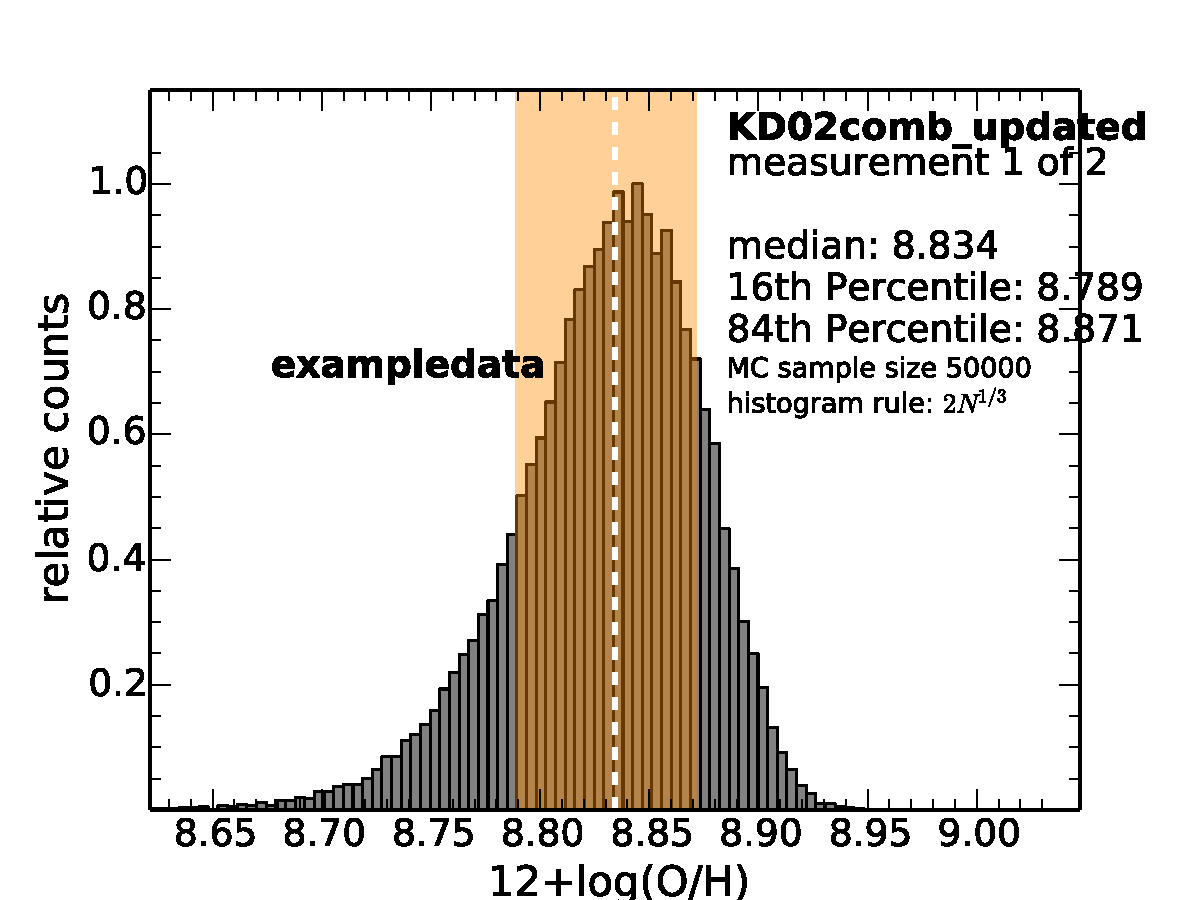
\includegraphics[width=0.95\columnwidth]{exampledata_n50000_KD02comb_updated_1.ps}
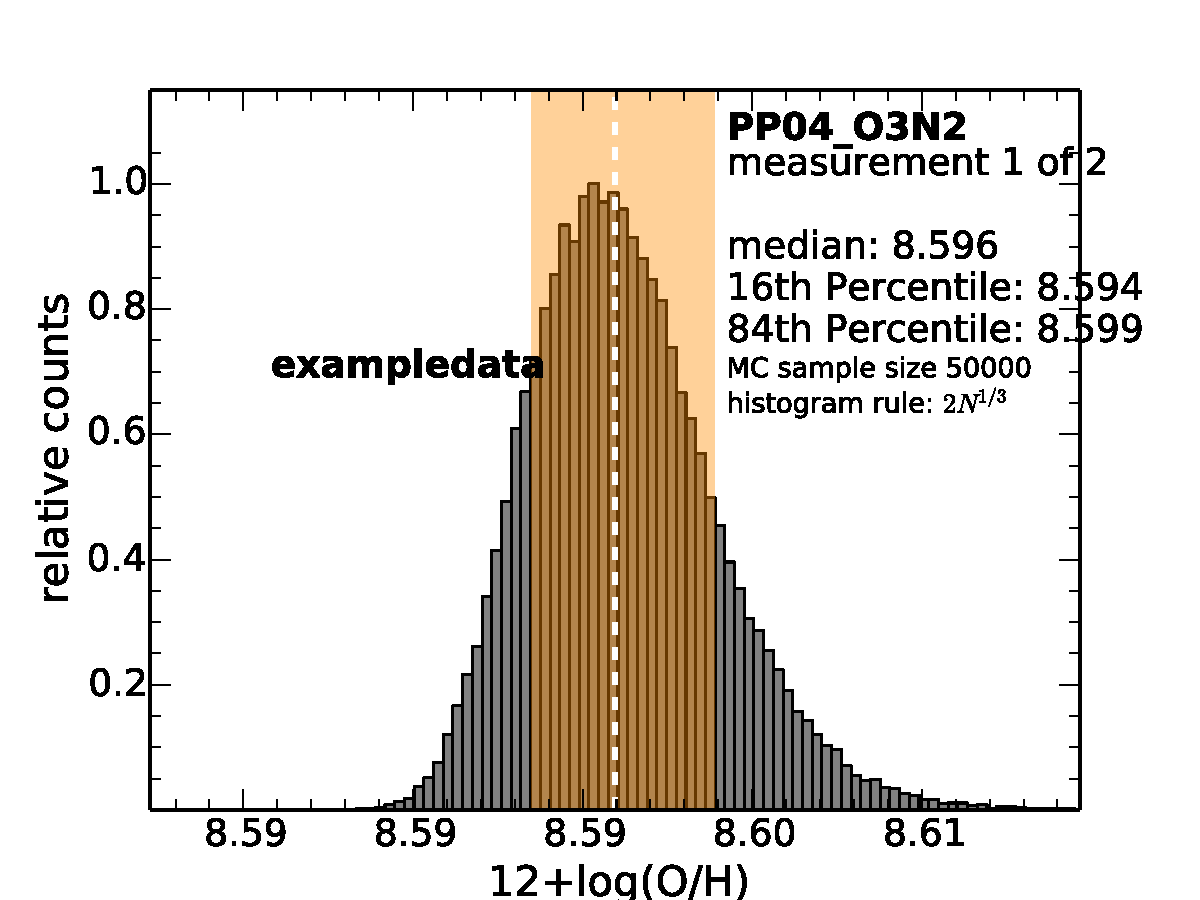
\includegraphics[width=0.95\columnwidth]{exampledata_n50000_PP04_O3N2_1.ps}
}
\vspace{0.2in}
\centerline{
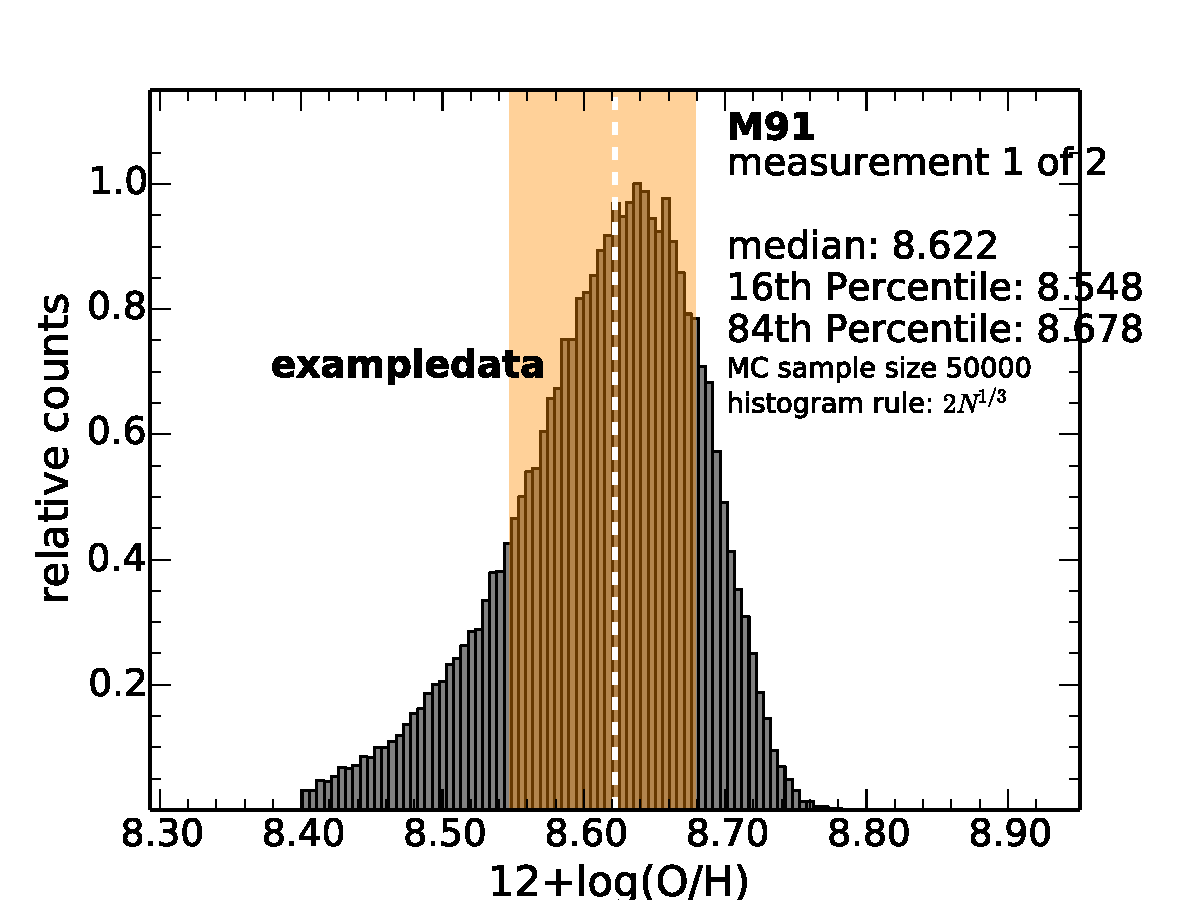
\includegraphics[width=0.95\columnwidth]{exampledata_n50000_M91_1.ps}
\includegraphics[width=0.95\columnwidth]{exampledata_n50000_E(B-V)_1.ps}
}
\caption{WILL UPDATE WITH NEW FIGURES BASED ON A PUBLISHED SN WITH SIGNFICANT E(B-V) AND WRITE MORE TEXT. Examples of confidence region determined by the algorithm, shaded in tan color.}
 \label{metallicity_distribution}
\end{center}
\vspace{-0.5in}
\end{figure*}


For computing oxygen abundances, we use the iterative code by Kewley \& Dopita (2002), which has been updated in \citet{kewley08} and reflects .. \textbf{LISA: YOUR INPUT HERE:what is the update??} which was initially written in IDL.  We translated it into python, added the new feature of obtaining uncertainties on the metallicity outputs via Monte Carlo resampling, and made it open source via github, as we explain below.

We assume that the observed emission lines to be used to indicate metallicity originate in HII regions and are not due to non-thermal excitation by e.g., AGN or interstellar shocks from SNe or stellar winds.  Tests to exclude data contaminated by such non-thermal sources have to be executed by using the recommended line ratios by e.g., \citealt{baldwin81,kauffmann03,kewley06_sdss} prior to running this code. Furthermore these lines should have all the correct calibration (at least correct relative calibration) and should have a signal-to-noise ratio (S/N) of at least 3. The latter is important for the success of the Monte Carlo resampling technique as described below.

\subsection{Input and Output of code}
Emission line flux values are fed into our Python implementation as in the original code by Kewley \& Dopita, which is written in IDL and hereafter referred to as IDL02. The inputs are emission line flux values and their uncertainties for the following lines: H$\alpha$, H$\beta$, [OI] 6300, [OII] 3727, [OIII] 4959, [OIII] 5007, [NII] 6584, [SII] 6717, [SII] 6731, SIII 9532, and SIII 9096 \textbf{CHECK!} and their uncertainties. If the fluxes for the specified lines are not available, the entry is left to 0 and the outputted oxygen abundance scales will be in only metallicity scales that use the line fluxes provided. As part of the code, the inputted line fluxes are corrected for reddening by using the observed Balmer decrement, for which H$\alpha$ and  H$\beta$ flux values are needed to be provided. We assume case B recombination and thus, the standard value of 2.86 as the
intrinsic H$\alpha$/H$\beta$ ratio \citep{osterbrock89}, and apply the standard Galactic reddening law with $R_V$ = 3.1 \citep{cardelli89}. However, the user can choose other extinction laws and $R_V$ values, if desired, given the code's open-source nature.

While other parameters, such as the ionization parameter $q$ and the electron density (using the $SiII$ lines) are computed as long as the necessary lines are provided, they are not outputted in the current version of our code $-$ however, the reader is welcome to easily modify the code to suite their needs, given it's an open-source code.

As output, we obtain metallicity values and their uncertainties in the following calibrations, as discussed in detail in \citet{kewley02,kewley08}: \citet{kewley02}(KD02, for the 4 following computations: R23, using the NIIOII ratio, using the NII/Halpha ratio, and a combined method that uses the optimal method given the input line fluxes), \citet{mcgaugh91} (M91), \citet{zaritsky94} (Z94), \citet{pilyugin01} (P01), \citet{denicolo02} (D02), 
\citet{pettini04} (2 computations: PP04-N2, PP04-O3N2) \textbf{CHECK WITH FINAL CODE}. If the line fluxes necessary for specific scales are not provided, the output  metallicities will -1    \textbf{CHECK WITH FINAL CODE}.



\subsection{Computing Uncertainties}
The novel aspect of our work is that we introduce a Monte Carlo (MC) resampling method to obtain numerous iterations via random sampling to obtain a more robust result for error estimation (e.g., \citealt{efron79,hastie09,andrae10}. Given a data set with error bars from which certain parameters are estimated, Monte Carlo resampling consists of resampling the data from its error distribution to produce alternative data sets. Here we generate a distribution of possible inputs by generating a gaussian error distribution centered on the measured line flux value, with a standard deviation corresponding to the measurement error, where we have made the assumption that the line flux error is gaussian distributed in nature\footnote{In case the user provides their own probability distribution for the emission line uncertainties (e.g. from fitting Gaussians to the emission lines via MCMC methods, the user is welcome to easily modify the code to suite their needs, given its open-source nature}. Every iteration randomly takes an input value from this distribution (for each inputted line) to run the calculations. This effectively simulates conducting multiple experiments when repeated observation is impractical or impossible, as in the case of the emission line flux data, and thus generates alternative data sets. We generated $N$ Monte Carlo samples of emission line fluxes (where an appropriate value of $N=50,000$ is determined below) and calculated the metallicity for each set of line fluxes. At the end of $N$ iterations, a parameter estimate distribution of oxygen abundance is generated for each scale by binning the results to histograms, and metallicity confidence regions are measured  (see below)\footnote{However, note this method is a conservative approach, since it overestimates the intrinsic metallicity uncertainty, as we are centering this error distribution on the measured values instead of the (unknown) true values \citep{andrae10}.} . This is done for each scale. The fiftieth (50\%) percentile, i.e.  the median, is reported as the measured value. The output of our code includes the oxygen abundance measurements plus confidence regions in all scales, as well as plots of the likelihood distributions of the oxygen abundance value in all scales. 
Figure \ref{metallicity_distribution} shows the metallicity estimate distribution for 4 representative scales - those are the same plots that are outputted as part of our code for all scales (not all shown here). As can be seen, the metallicity distributions are rarely Gaussian, for two reasons: first, since the metallicities are computed based on log values of line flux ratios, symmetric error bars in linear space will translate into asymmetric error bars in log space; and seconds, since some metallicity computations (especially those that include $R_{23}$) are non-linear since they choose an upper vs lower branch by breaking the degeneracy.

This MC resampling approach takes into account the impact of the uncertain reddening (due to the uncertainties in the measurement of the 
H$\alpha$ and H$\beta$ fluxes), when the option for de-reddened metallicities is chosen. Since for each iteration, a new reddening value is calculated based on the resampled H$\alpha$ and H$\beta$ fluxes, which is used to compute the de-reddened metallicity value, the derived distribution of metallicity values takes into account the uncertain redding. As part of the optional output, a probability distribution plot for E(B-V) is provided (see last plot in figure~\ref{metallicity_distribution}, along with confidence intervals derived using the same method as for the metallicity measurements. If either H$\alpha$ or H$\beta$ flux is not provided, then no reddening correction can be applied and the computed metallicity will not be  reddening-corrected and the E(B-V) output will be set to blank.

We note that our code  does not output the \emph{systematic} uncertainty of each scale, which are e.g., $\sim$ 0.07 dex (or 0.14 dex \textbf{CHECK}) for PP04-O2N2.  Thus systematic errors can be as large, if not larger, than the statistical errors, however, if all metallicity measurements are in the \emph{same} scale and only \emph{relative} comparisons are made, then the systematic error does not have any impact (by definition!). 

%However, the
%relative metallicity difference measured between a given pair
%of galaxies in different diagnostics is consistent with an rms
%scatter typically ?0.07 dex, and 0.15 dex between the most
%discrepant diagnostics (Kewley&Ellison 2008).


%from Kewley & Ellison08: The cause of the metallicity calibration discrepancies remains unclear. The discrepancy has been attributed to either an unknown problem with the photoionization models (Kennicutt et al. 2003) or temperature gradients or fluctuations that may cause metallicities based on the electron temperature method to underestimate the true metallicities (Stasin�ska 2002, 2005; Bresolin 2006). Until this discrepancy is resolved, the absolute metallicity scale is uncertain.

\subsubsection{Histogram Bin Size and Confidence Region}

Choosing the binning for a histogram is not trivial and \citet{hogg08} describes various data analysis recipes for selecting a histogram bin size. Too many bins will result in many empty bins and an "over-fit" histogram, while too few bins may lose features of a probability distribution. While for our default option, we use Rice Rule (e.g., \citealt{hastie09}), namely using $2* \sqrt[3]{N}$ as a number for our bins (which was appropriate for most of our test cases), we enable a number of binning options from which the user can choose, including Bayesian blocks, Knuth's rule and Doane's formula (\textbf{Fed's input here!}).

%Using a bin size of $\sqrt{N}$ was recommended, but this proved to be slightly over-fitting, and after a number of tests, we found $2* \sqrt[3]{N}$ to be appropriate for most cases.

Since the metallicity distributions are rarely Gaussian, we cannot just fit a Gaussian and report the 1-$\sigma$ intervals. In determining the confidence region intervals for asymmetric and multi-modal distributions, there are broadly three approaches (e.g., \citealt{andrae10}): choosing a symmetric interval, the shortest interval , or  a central interval.  We determined the confidence interval using the ``central" method, because it ensures that the algorithm finds the proper boundaries even in the case of multiple peaks (i.e., multimodal likelihood distributions) and for asymmetric, non-Gaussian, distributions. With the "central" method we determined the  confidence interval by choosing the left and right boundaries such that the region outside the confidence interval each equally contains $16\%$ of the total distribution for one standard deviation confidence interval - in analogy to the one-sigma-interval of the Gaussian distribution. 
 While the histograms at sufficiently high $N$, where $N$ is the total number of iterations, yielded single peaked results, at lower $N$ there were occasional multiple peaks resulting from a non-smooth gaussian being sampled. In selecting the value of $N$, we found that around $N=50,000$ provides reliably smooth histograms. 

In summary, the output for the measured value corresponds to the fiftieth (50\%) percentile, while the lower error bar corresponds to the 50$^{th}$-16$^{th}$ percentile and the upper error bar corresponds to 84$^{th}$-50$^{th}$ of the metallicity parameter estimate distribution. However, we urge that the reader always inspect the appropriate metallicity distribution plots, which are also outputted, to check for themselves whether the outputted median and confidence regions properly represent the full metallicity distribution.





\section{Comparison to prior uncertainty computation and other works }\label{comp_sec}


A previous method for determining the uncertainty in the oxygen abundance (as used in \citealt{modjaz08_Z,kewley10,rupke10,modjaz11}) was an \emph{analytic} approach of propagating the emission-line flux uncertainties: it found the maximum and minimum abundances via maximizing and minimizing, respectively, the various line ratios by adding/subtracting to the measured line values their uncertainties. For comparison we computed the metallicities and their errors in both ways (both analytic and using our current MC resampling method) for 3 representative scales. We plot our results and the residuals in Fig.\ref{comp_anal_MC}, which shows a number of important points: i) The metallicity reported as the 50th percentile of the metallicity parameter distribution from the MC resampling method is completely consistent with the analytically derived metallicity -  well within the respective error bars - and thus, the prior published results still stand. ii) The MC resampling method has smaller error bars than the analytic method, especially for the scales of M91 and KD02. This is easily understandable, since the analytic method assumes the worst-case-scenario, as it basically yields 2 metallicity parameter draws (the "minimum" and "maximum") which are in the tail of the full metallicity probability/likelihood distribution. However, the MC resampling method is the more appropriate method as it empirically characterizes the full parameter estimation distribution.
%assumes that \textbf{all} emission line measurement have been drawn from the 68\% tail of the error distribution and 

\begin{figure}[ht!]
%  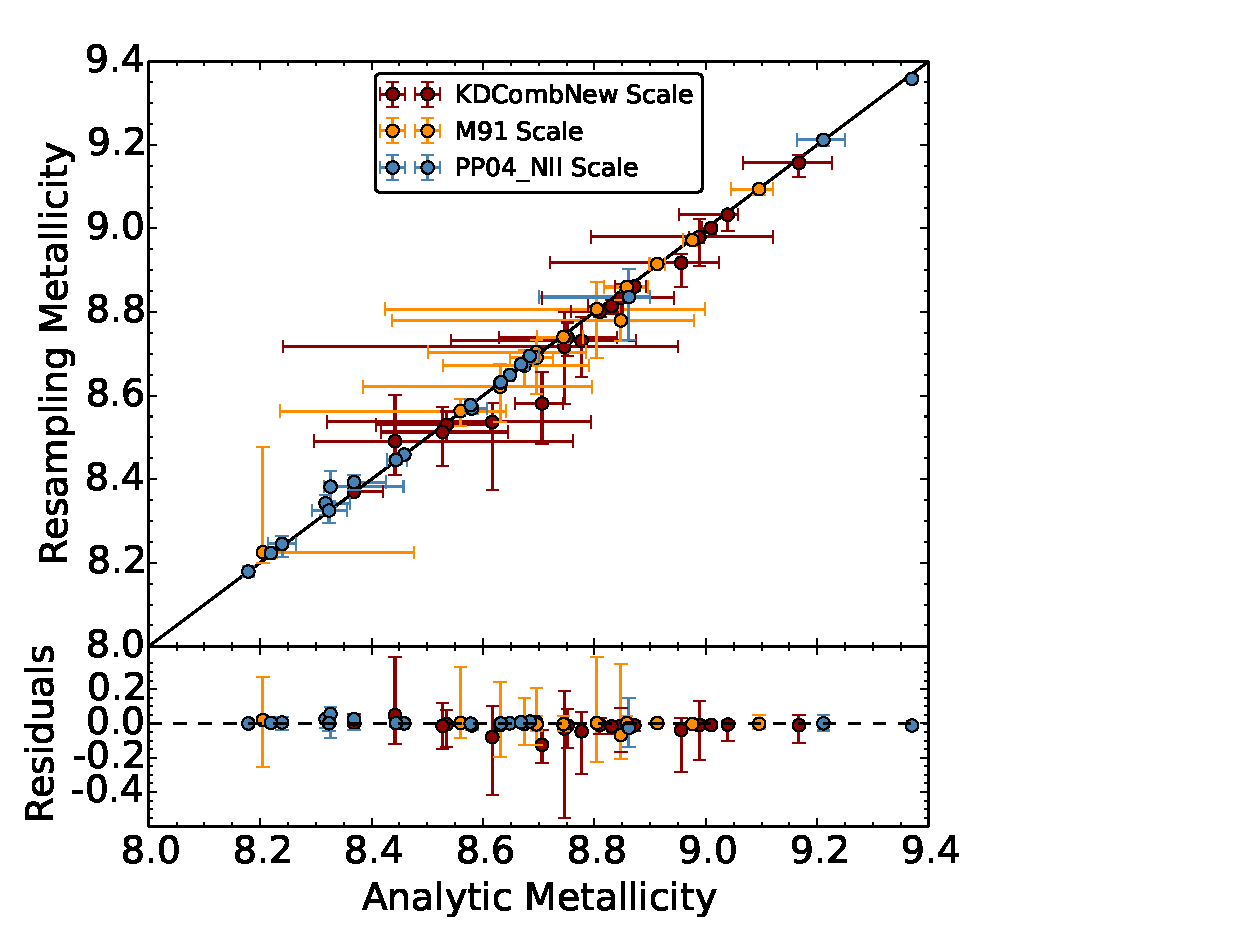
\includegraphics[trim = 10mm 0mm 10mm 0mm, clip]{abcomparison6.eps}
  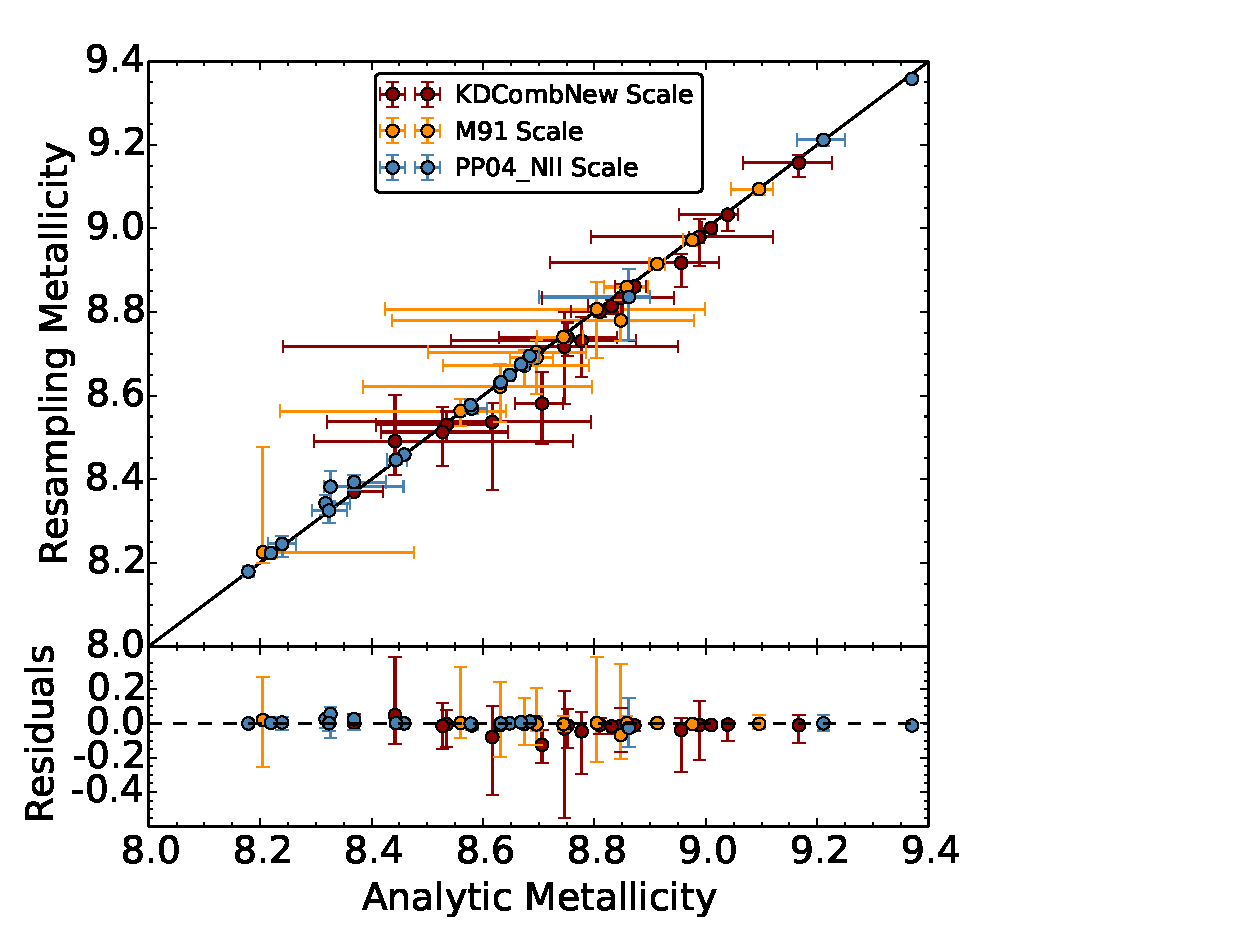
\includegraphics[width=1.2\columnwidth]{abcomparison6.eps}
   \caption{\textbf{FINISH}.Comparison of metallicity estimation between the analytic method and our Monte Carlo resampling method (top) and their residuals (bottom) for 3 different metallicity scales. Flux measurements come from 19 galaxies previously measured in \citet{modjaz11}. To add asymmetric errors in quadrature we use $residual_{min}=\sqrt {x_{max}^2 + y_{min}^2}$ and $residual_{max}=\sqrt {x_{min}^2 + y_{max}^2}$.}
 \label{comp_anal_MC}
\end{figure}

%Although the flux probability distribution function is assumed to be symmetric, the metallicity errors are asymmetric because they are derived from the log of minimized and maximized flux ratios.
%Rupke: Errors were propagated primarily using analytic expressions, but for abundance and gradient errors we employed Monte Carlo methods.

\subsection{Comparison with other works}

%Here we perform a literature review of both 


The field SN host metallicity studies has been rapidly developing as these kinds of studies may be crucial avenues for constraining the progenitor systems of different kinds of explosions- however, many of the works do not show how they compute their statistical errors (e.g., \citet{anderson10,leloudas11,sanders12,leloudas14}). While \citet{sanders12} compute the line flux errors from a Markov-Chain Monte Carlo fitting of a gaussian to the emission lines, they only mention in passing that they propagate the line flux uncertainties into the metallicity measurements, but do not describe how.

%by propagation of the uncertainties in the line flux measurements
%and the 0.07 dex diagnostic systematic error.
%( line flux errors from MCMC fitting of a gaussian to emission lines)

In contrast, the general metallicity field has considered in detail how to estimate the uncertainties in measured metallicities- however, none of those codes are open-source and many of them are for specific scales which were chosen by the authors:  \citet{moustakas10} also use MC resampling to estimate the metallicity uncertainties (in their case using 500 trials which seems to lead to a Gaussian distribution) but only do this for two scale, KK04 and \citet{pilyugin05}. For computing the metallicities of the SDSS star forming galaxies, \citet{tremonti04} fit a combination of stellar population synthesis and CLOUDY photoionization models to the observed strong emission lines [OII], Hbeta, OIII, Halpha, NII and SII and report the median of the metallicity likelihood distribution as the metallicity estimate, with the width of the distribution giving the 1 $\sigma$ (Gaussian) error. However, this is constitutes their own scale, the T04 scale.

In the last stages of preparing this manuscript \citet{blanc15} was published.  \citet{blanc15} employ Bayesian inference for doing something similar to \citet{tremonti04} - they use Bayesian inference to derive the joint and marginalized posterior probability density functions for metallicity and ionization parameter $q$ given a set of observed line fluxes and an input photoionization model. They provide a publicly available IDL implementation of their method named $IZI$ (inferring metallicities (Z) and ionization parameters) on the author's website.


\section{Conclusions}\label{comp_sec}

 \textbf{FINISH}. We hope that this open-access code will be used in many different fields where gas-phase metallicities are important, including in the emerging field of SN and GRB host galaxies, where either it is not described how they got  or no error bars are computed (e.g., \citealt{lunnan14}).

\acknowledgements
M. Modjaz is supported in parts by the NSF CAREER award AST-1352405 and by NSF award AST-1413260. 
 This research made use of NASA�s Astrophysics Data
System; the NASA/IPAC Extragalactic Database (NED), which
is operated by the Jet Propulsion Laboratory, California Institute
of Technology, under contract with the National Aeronautics
and Space Administration.



%\epsscale{1.0}
%\begin{center}
%\csvautotabular{table1.csv}
%\label{t1}
%\caption{Comparison of M-M method with MC method}
%\end{center}
%\end{figure*}



%%%%%%%%%%%%%%%%%%%%%%%%%%%%%%%%%%%%%%%%%%%
%%\clearpage
%%%%%%%%%%%%%%%% BIBLIOGRAPHY  %%%%%%%%%%%%%%%%%%%%%%%% 
\bibliographystyle{apj}
%\bibliography{refs}
\bibliography{/Users/maryammodjaz/Dropbox/refs}

\appendix

\section{Minimum Code validation}
\textbf{WORK WITH FED - and any other code specific things}
\end{document}
%,page]{appendix}
%\usepackage{amsmath}
%\usepackage{amssymb}
%\usepackage{verbatim}
%\usepackage{graphicx}
%\usepackage{epsfig}
%\usepackage{morefloats}
%\usepackage{float}
%\usepackage{lipsum}
%\usepackage{subfigure}
%\usepackage{longtable}
%\usepackage{lipsum} 
%\usepackage{rotating}
%\usepackage{wasysym}

\begin{document}
\title{Monte Carlo Method for Calculating Oxygen Abundances and Their Uncertainties from Strong-Line Flux Measurements}

\author{Federica B. Bianco\altaffilmark{1}, Maryam Modjaz\altaffilmark{1}, Seung Man Oh\altaffilmark{1,2}, David Fierroz\altaffilmark{1}, Yuqian Liu\altaffilmark{1}, Lisa Kewley\altaffilmark{3,4}}
\altaffiltext{1}{Center for Cosmology and Particle Physics, New York University, 4 Washington Place, New York, NY 10003, USA}
 \altaffiltext{2}{NYU Abu Dhabi PO Box 129188 Abu Dhabi, UAE}
 \altaffiltext{3}{Australian National University, Research School for Astronomy \& Astrophysics, Mount Stromlo Observatory, Cotter Road, Weston, ACT 2611, Australia }
 \altaffiltext{4}{ Institute of Astronomy, University of Hawaii, 2680 Woodlawn Drive, Honolulu, HI 96822, USA}
 
 
\begin{abstract}
We present the open-source Python code \verb=MCZ= for the determination of the strong-emission-line estimators of oxygen abundance in the standard scales, based on the original IDL-code in \citet{kewley02}, and expanded to include more recently developed scales. The standard strong-line oxygen diagnostics have been used in many areas of astrophysics, including galaxy evolution and supernova (SN) host galaxy studies, to estimate the oxygen abundance in the interstellar medium through various emission line ratios. Oxygen abundance is considered a proxy for total metal abundance, since Oxygen is the most abundant metal. 
%FED: broken the sentence above in 2 cause it was windy
Here we introduce a Python implementation of these methods that through Monte Carlo resampling  better characterizes the statistical reddening-corrected oxygen abundance confidence region.  Given line flux measurements and their errors, our code produces synthetic Monte Carlo distributions for the oxygen abundance simultaneously in a large number of currently-used metallicity scales 
%(11 scales, as well as their sub-scales, as a default and 3 additional scales upon request)
%FED: maybe  too much detail for the abstract: how about just 
in up to 33 scales and sub-scales, as well as for E(B-V), when possible, and estimates the median values and 16th and 84th percentile confidence regions, for each metallicity diagnostic and for the reddening parameter E(B-V). In addition, it has the option of outputting the full MC parameter distributions, as well as their kernel density estimates. We test our code on emission lines measurements from a sample of supernova host galaxies (with $z<0.15$) and compare our metallicity results with those from previous methods. We show that our metallicity estimates are consistent with previous methods but yield smaller uncertainties. We also offer visualization tools to assess the spread of the oxygen abundance in the different scales, as well as the shape of the estimated oxygen abundance distribution in each scale, and develop robust metrics for determining the appropriate MC sample size. 
%We furthermore perform benchmark calculations that includes computing the memory usage for different scales. 
The code is open access and open source, 
%parallizable, 
and it can be found at \url{www.github.com/nyusngroup/MC_Metallicity}.
\end{abstract}
 
\section{Introduction}
Small amounts of carbon, oxygen, nitrogen, sulfur and iron and other elements provide a splash of color to the otherwise dominating greyscape of hydrogen and helium in the stars and gas of galaxies. Nevertheless, even this minute presence of heavy elements (all elements heavier than H and He, also called metals or collectively metallicity) is important for many areas of astrophysics. For example, \citet{johnson12}, amongst others, suggest that if it was not for the relatively high metallicity level in our Solar System, planet formation may not have been possible. With $Z$ representing the mass fraction of metals, for our own Sun the value is measured to be  Z=0.0153 \citep{chaffau11}, though there suggestions for a lower solar metallicity of $Z=0.0134$  \citep{asplund09_rev,grevesse10}. 
Furthermore, when properly observed and estimated, metallicity measurements of galaxies can tightly constrain models of galaxy formation and evolution (e.g., \citealt{kewley08} and references therein), as well as shed light on the metallicity dependence and production conditions for different types of Supernovae (SNe) and long-duration Gamma-Ray Bursts (GRBs) (e.g., \citealt{modjaz08_Z,levesque10_grbhosts,anderson10,modjaz11,kelly12,sanders12,lunnan14,leloudas14,pan14}).

%chaffau Z=0.0209 12+log=O/H) = 8.76\pm0.07 
Most metals are produced in the cores of massive stars during their fusion life cycle but also during the extreme conditions of stellar explosions. For example, the majority of iron is synthesized in thermonuclear explosions (SNe Ia) while nearly all of oxygen and other $\alpha$-elements are released in various kinds of core collapse SNe (SNe II and stripped-envelope core-collapse SNe). Since new stars are born from the clouds these explosions enrich, metallicity will increase with each passing generation of stars. 

%Besides age, metallicity also influences stellar temperature. Metals are more effective at absorbing energy coming from the interior of the star in the stellar atmosphere so their presence increases the stellar opacity. With greater absorption and opacity the radius expands to a size larger than it would be without metals and this larger size results in a cooler effective temperature. While metallicity can help indicate age or activity it's temperature and density dependencies require parameterization to properly be estimated.

However, for almost all astronomical objects, metallicity cannot be measured directly. The oxygen abundance in the gas-phase is the canonical choice of metallicity indicator for interstellar medium (ISM) studies, since oxygen is the most abundant metal and only weakly depleted onto dust grains (in contrast to refractory elements such as Mg, Si, Fe, with Fe, being depleted by more than a factor of 10 in Orion; see \citealt{simondiaz11-orion}). The oxygen abundance\footnote{We note that in many cases in the literature, including here, the terms metallicity and oxygen abundance are used interchangeably.} is expressed as  \oxab, where $O$ and $H$ represent the number of Oxygen and Hydrogen atoms, respectively. In particular, \citealt{chaffau11} measure a solar oxygen abundance of \oxab = 8.76 $\pm$ 0.07, while \citet{asplund09_rev} suggest \oxab = 8.69.

Importantly, oxygen exhibits very strong nebular lines in the optical wavelength range in spectra of HII regions (e.g., \citealt{pagel79,osterbrock89,tremonti04}), which can be measured. Thus, many different diagnostic techniques, relying on different lines of oxygen, hydrogen and other elements, have been developed (e.g., \citealt{kewley02,pettini04,kobulnicky04,kewley08}), which are discussed in the next section. Ultimately, the purpose of this paper is to present a public code that computes the metallicity from strong emission line fluxes according to the many different abundance diagnostics as well as the associated statistical uncertainties due to the measured emission line flux uncertainties.

\subsection{The different oxygen abundance diagnostics}

Here we present a brief overview of the various observational methods for measuring the gas-phase oxygen abundance - however, for a detailed discussion, and to understand the many caveats, we encourage the reader to read the reviews by e.g. \citet{stasinska02,kewley08,moustakas10,stasinska10,dopita13,blanc15}.
The so-called ``classical'' way to estimate the oxygen abundance is the electron temperature ($T_e$) method, which estimates the electron temperature and density of a nebula using a number of oxygen lines with different ionization states, including the auroral [OIII]~$\lambda$4363 line, to then directly estimate the OII and OIII abundances and finally obtain the total oxygen abundance, after correcting for the unseen stages of ionization. However, the auroral [OIII] $\lambda$4363 line is very weak, except in low-metallicity environments, and saturates at higher metallicity (since at higher metallicities the cooling is dominated by the oxygen NIR fine structure lines)
%\footnote{Note however, that most recently \citet{berg15} suggest that [OIII] $\lambda$4363 line is the most problematic auroral line to use amongst those of [OII], [OIII] [NII], [SII], [SIII], giving rise to temperature discrepancies.} 
$-$ thus, other methods had to be developed that use other, stronger lines in the spectra of HII regions. These are called \emph{strong-line methods} and are the subject of this manuscript. Strong-line methods can be categorized into two types: theoretical methods, that rely on calibrating various observed line ratios using photoionization methods (basically theoretically simulating HII regions, using stellar model atmospheres, stellar population synthesis and photoionization models) and empirical ones, that calibrate various observed strong line ratios using observed $T_e$-based metallicities. While historically there have been large systematic offsets between the $T_e$ method and the strong line methods, \citet{dopita13} demonstrated that the $T_e$ method gives the same results as the strong line methods, if the energy distribution of the electrons in the HII regions is assumed to not be a simple Maxwell-Boltzmann distribution (as assumed in prior works), but a more realistic $\kappa$ distribution, as observed in solar system astrophysical plasma. They also find that the effect of changing the specific $\kappa$ distribution on the strong-line methods is minor. 

%For strong-line methods, there are again two classes of methods: those that calibrate the metallicity based on theoretical model grids that include stellar population plus photoionization (called "theoretical methods"), and those that that are empirical which use $Te$-measured metallicities for calibration (called "empirical methods"). 
For theoretical strong-line method, a ratio of oxygen line fluxes to $H\beta$, referred to as $R_{23}$, is commonly used to determine the metallicity of galaxies  \citep{pagel79}:
$$R_{23}=\frac{\mathrm{[OII]} \lambda 3727~+~\mathrm{[OIII]} \lambda 4959,\lambda 5007}{\mathrm{H}_\beta},$$ 
where [OIII]$\lambda$4959,$\lambda$5007 stands for the sum of the two [OIII] lines.
The drawback of this method is that is double-valued with metallicity: the same $R_{23}$ value may correspond to two metallicity values, and thus other line ratios need to be used to break the degeneracy between the high values ("upper branch") and the low values ("lower branch") of the $R_{23}$ metallicities (e.g., \citealt{kewley08},  \citealt{moustakas10}). 
Furthermore, \citet{kewley02} showed the importance of ionization parameter, which can be physically understood as corresponding to the maximum velocity of an ionized front that can be driven by the local radiation field of hot massive stars that are ionizing the ISM gas. This ionization parameter needs to be taken into account in the various strong-line methods, as HII regions at the same metallicity but with different ionization parameters produce different line strengths. Calibrations of $R_{23}$ by \citet{mcgaugh91} (hereafter M91), by \citet{kewley02} (hereafter KD02), and by \citet{dopita13} (hereafter D13) use different theoretical photoionization models and take the ionization parameter into account, while other calibrations such as that of \citet{zaritsky94} (hereafter Z94) do not. Thus, Z94 is mostly valid for only metal-rich galaxies.  M91 and KD02 use an iterative process to break the $R_{23}$ degeneracy  (KD02 uses different ratios [NII]$/$[OII] and [NII]/\ha) and to also constrain the ionization parameter $q$ in order to arrive at the metallicity estimate.

%The most direct way to estimate metallicity in spectra is to measure line fluxes absorbed or emitted by metals and non-metals. While iron lines may be present in stellar spectra, iron is less commonly found in gaseous nebulae than oxygen is. Not only is oxygen more abundant but it emits several strong lines ([OI] $\lambda 6300$, [OII] $\lambda 3727,7318,7324$, [OIII] $\lambda 4363, 4959, 5007$) visible at optical wavelengths that can also be used to quantify temperature and density. For this reason 
%While the ratio of oxygen to hydrogen line flux correlate with metallicity, the ratio of two [OIII] lines, one auroral $\lambda 4363$ and the other an excitation line at $\lambda 5007$ can be used to determine what is called the Ionization Correction Factor (ICF) (Kewley \& Dopita 2002).
As to empirical strong-line methods, the most commonly used ones are those by \citet{pettini04} (hereafter PP04), \citet{pilyugin05} (hereafter P05) and \citet{marino13} (hereafter M13). PP04 used HII regions with measured $T_e$-based metallicities to derive empirical fits to strong-line ratios, and introduced the line ratios of $\frac{\mathrm{[NII]}}{\mathrm{H}\beta}$ ($N2$) and $\frac{\mathrm{[OIII]}}{\mathrm{H}\beta} / \frac{\mathrm{[NII]}}{\mathrm{H}\alpha}$ ($O3N2$) as metallicity diagnostics. Since PP04\_N2 employs two closely spaced lines (\ha~ and NII), which are not affected by stellar absorption, nor (uncertain) reddening, and are easily observed in one simple spectroscopic setup, it has become an popular scale to use, at least for low-z SN host galaxy studies (see meta-analysis by e.g,. \citealt{sanders12,modjaz12_proc,leloudas14}). However, it is important to remember that this scale has a number of short-comings: it does not take into account the impact of the ionization parameter, it was initially derived based on only 137 extragalactic HII regions, and the nitrogen emission line employed saturates at high metallicity, and thus the PP04\_N2 method saturates for high-metallicity galaxies (at $\oxab > 8.8$, \citealt{kewley08}). An updated calibration by \citet{marino13} (whose scale our code also outputs, see below) based on many more $T_e$-based metallicities (a sample almost three times larger than that of PP04) derives a significantly shallower slope between $O3N2$ index and oxygen abundance than the PP04 calibration. In addition, most recently, \citet{berg15} suggested that the auroral [OIII] $\lambda$4363 line, commonly used for $T_e$ measurements, is the most problematic auroral line to use amongst those of [OII], [OIII] [NII], [SII], [SIII], giving rise to temperature discrepancies.


As it can be seen, each scale has different advantages and disadvantages and should be used in different metallicity regimes (see detailed discussion in e.g.,  \citealt{kewley02,stasinska02,kewley08,moustakas10,lopezsanchez12,dopita13,blanc15}). Thus, this open-source code outputs the oxygen abundance in the main (13 as of version v1.0, Spring 2015) metallicity scales (with the KD02 diagnostic having four outputs and the PP04, P10, M13 , M08, and D13  diagnostic having multiple outputs as well). While there is a long-standing debate about which diagnostic to use, as there are systematic metallicity offsets between different methods (recombination lines vs. strong-line method vs. ``direct'' $T_e$ method, see the above sources), \emph{\bf the relative metallicity trends can be considered robust, if the analysis is performed self-consistently in the same scale, and trends are seen across different scales \citep{kewley08,moustakas10}}. Thus, it is then necessary to obtain statistical error bars for the relative comparisons to be meaningful. Note however, that while there are conversion values between different scales \citep{kewley08}, they apply for large data sets, since those conversion values were derived based on ten thousands of SDSS galaxies, and thus should be used with caution (or not at all) for smaller samples.
%FED this is not strictly correct: you do want to derive conversions from large samples, but what you are saying is that you do not know about the spread of the conversion distribution, and thus you do not know how much individual data points could deviate. Is that not stated in the papers that derive the conversions??.
In addition, one should note that on account of the ongoing debate about the value of the solar oxygen abundance \citep{asplund09_rev,chaffau11}, that the absolute oxygen calibration is still uncertain.



Here we introduce the open-source Python package named \textbf{MCZ}.
%FED: python ``packages'' do not have the .py termination, cause they include multiple files, so just MCZ.  
This Python code allows the user to quickly produce metallicity values with sensible confidence regions for several metallicity scales at once, given an input set of spectral line measurements and their errors. While we do not mean to advocate for a particular metallicity scale to be adopted, the comparison of multiple scale outputs, and the shape of each metallicity distribution, can guide the user in understanding the reliability of a metallicity estimate, given a set of line fluxes. In \S~\ref{method_sec} we describe our method, and the input and output values of the code. We furthermore develop robust metrics for determining the appropriate MC sample size and perform benchmark calculations that includes computing the computer memory usage for many different scales. In \S~\ref{comp_sec}, we compare our method of obtaining abundance uncertainties to previous methods in the literature and conclude with \S~\ref{conclusions_sec}. 

%\begin{figure}[H]
%\epsscale{1.0} 
%\begin{center}
%\includegraphics[width=0.89\columnwidth]{fig1.png} 
%\caption{Example of a sampled Gaussian. 50,000 points from a Gaussian distribution were selected in this case}
%\label{f1}
%\end{center}
%\end{figure}


\section{Description of Metallicity code}\label{method_sec}


\begin{figure*}[!ht]
%\epsscale{0.6}
\centerline{
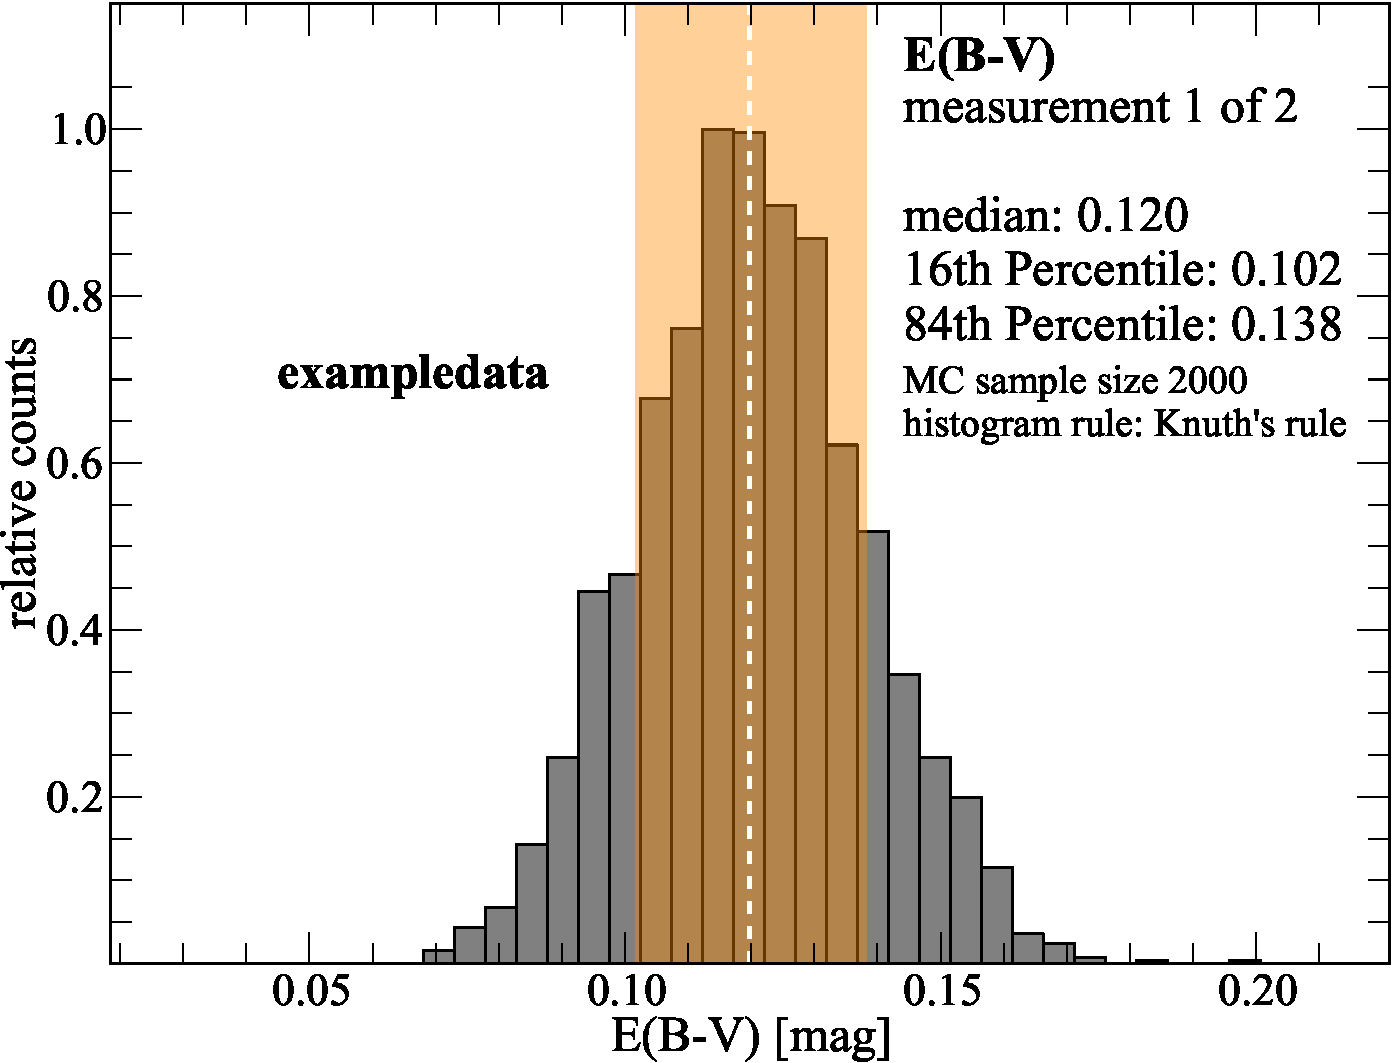
\includegraphics[width=0.98\columnwidth]{exampledata_n2000_EB-V_1.pdf}
%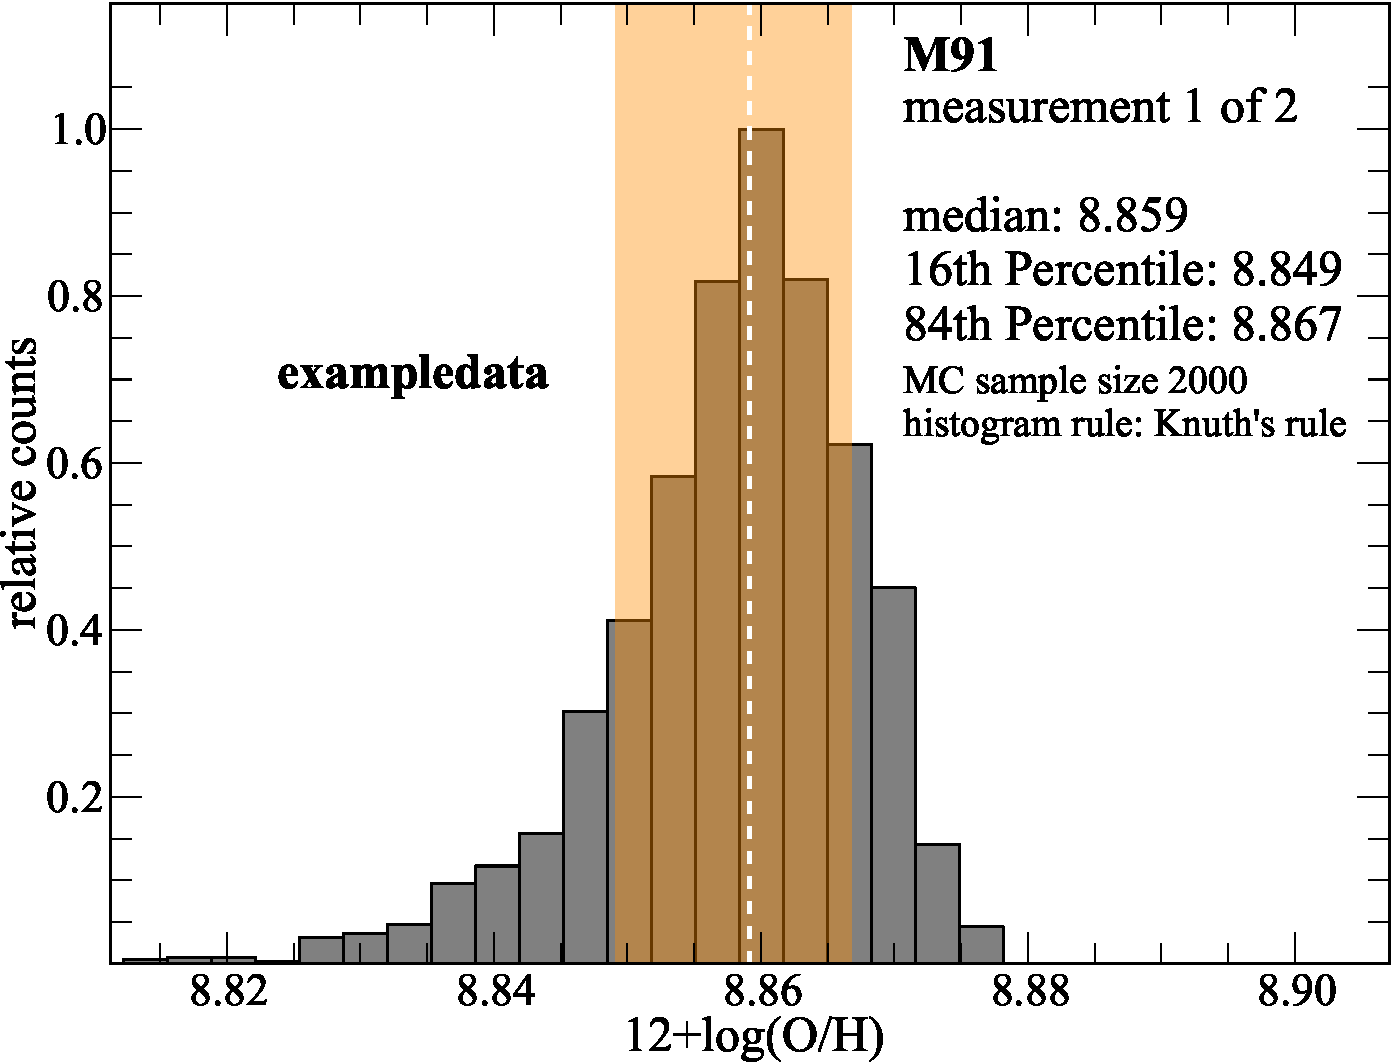
\includegraphics[width=0.98\columnwidth]{exampledata_n2000_M91_1.pdf}}
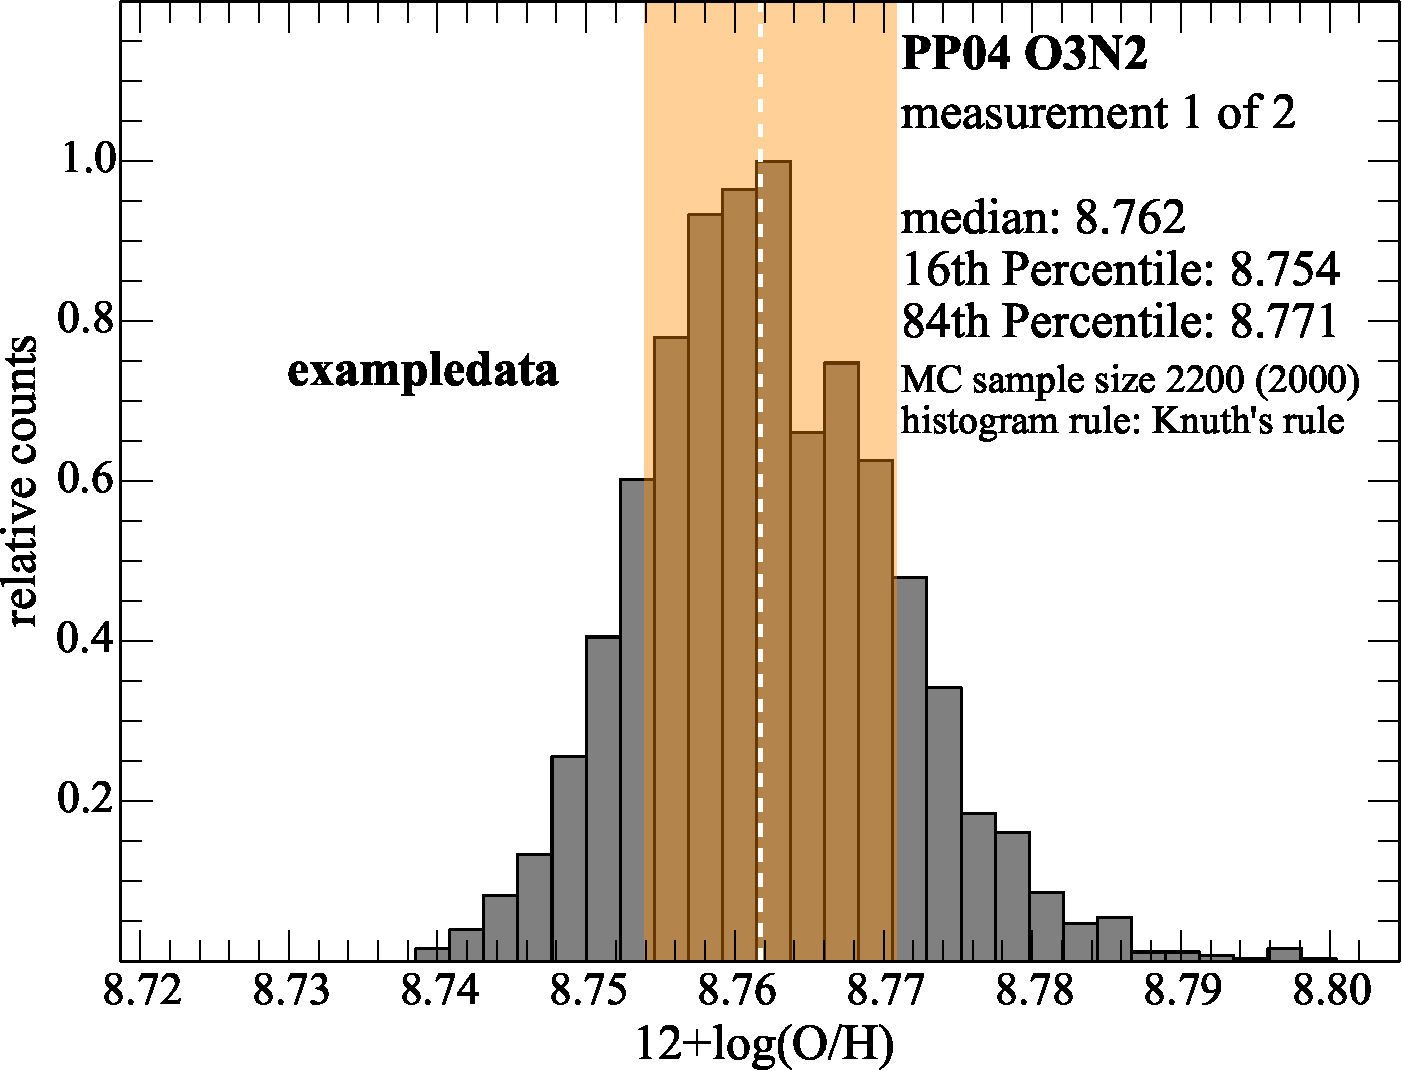
\includegraphics[width=0.98\columnwidth]{exampledata_n2000_PP04_O3N2_1.pdf}}
% exampledata_n50000_M91_1.ps}
%\vspace{0.2in}
\centerline{
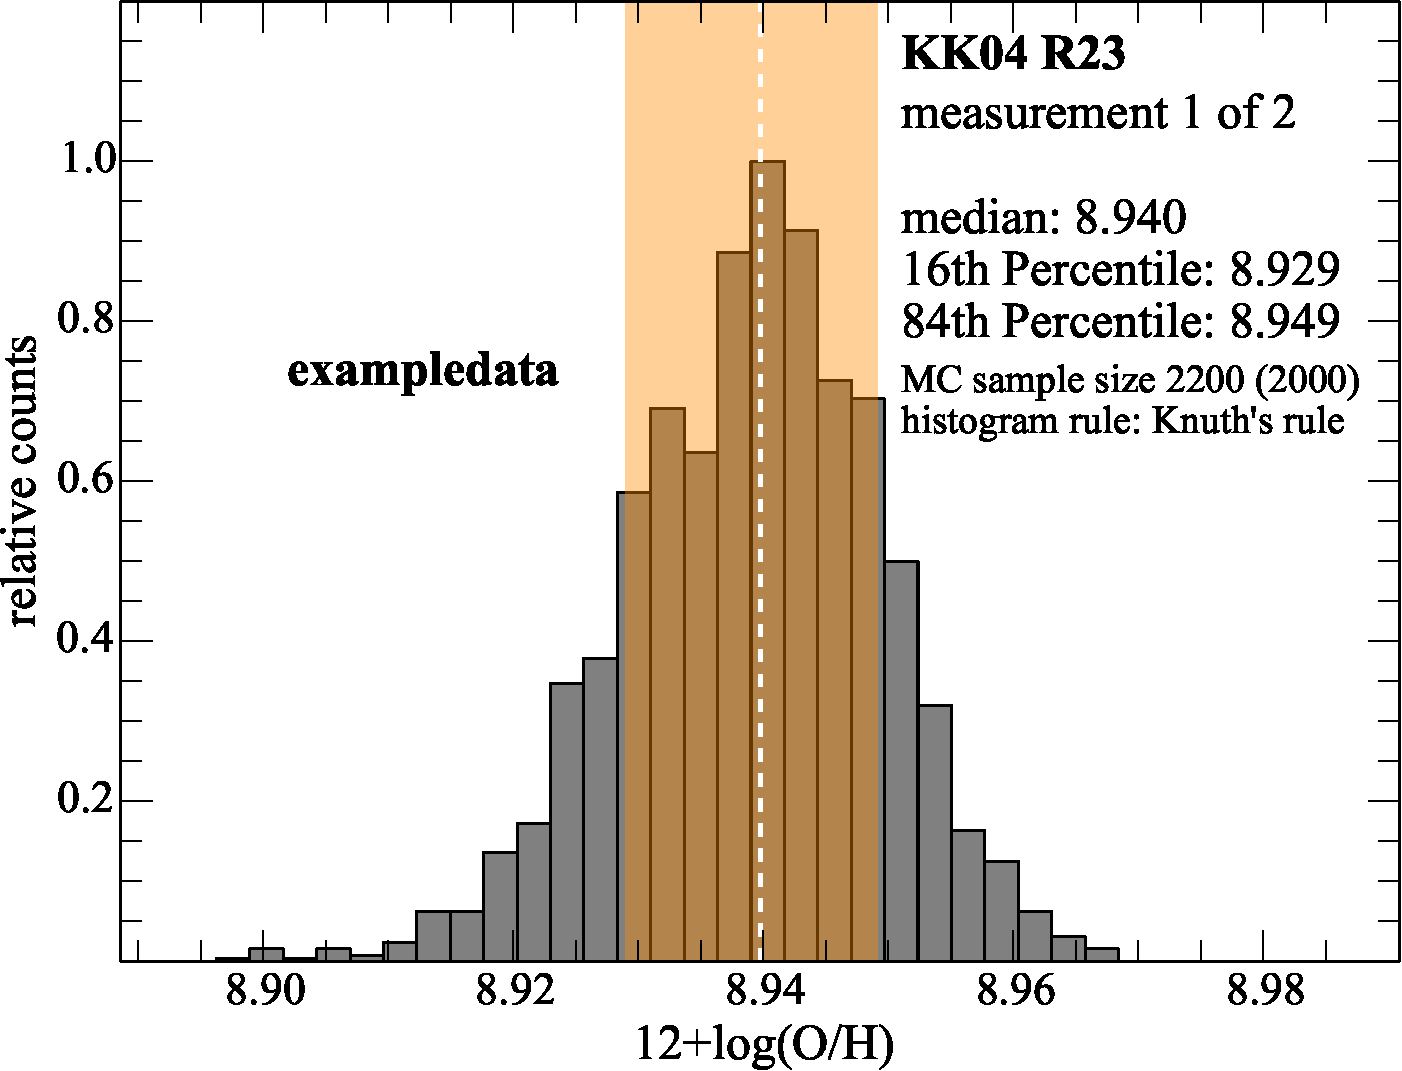
\includegraphics[width=0.98\columnwidth]{exampledata_n2000_KK04_R23_1.pdf}
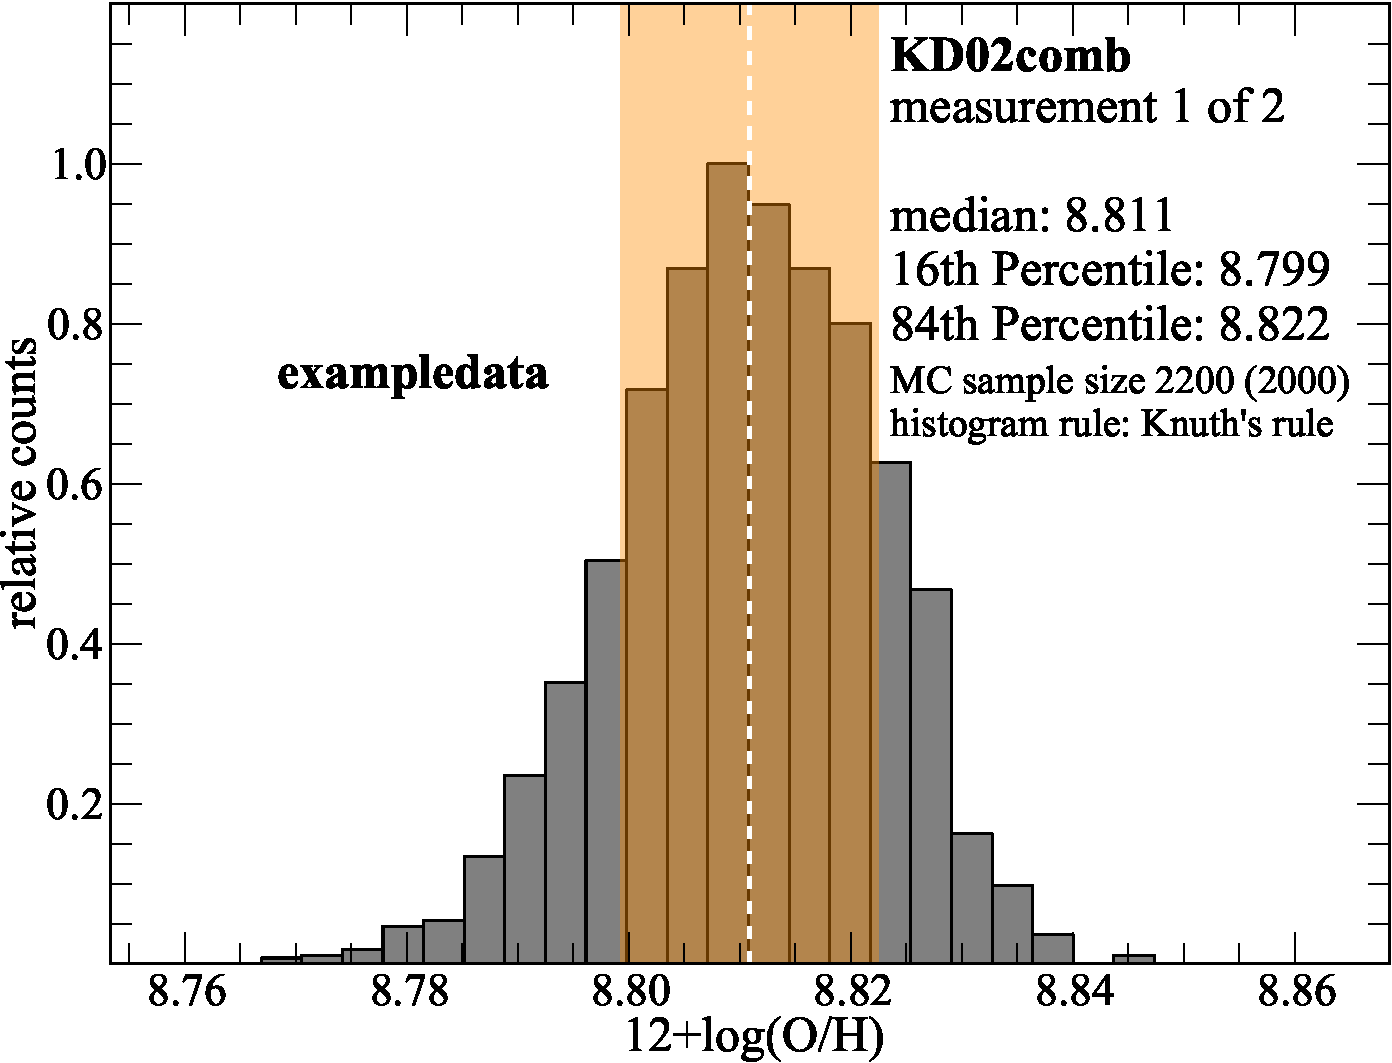
\includegraphics[width=0.98\columnwidth]{exampledata_n2000_KD02comb_1.pdf}}
\caption{Metallicity and reddening E(B-V) parameter distributions based on the example data shown in Table~\ref{tab:exampledata}: emission line data of the HII regions at the position of SN~2008D, published in \citet{modjaz11}. The distributions are generated from $N$=2,000 samples. The median values are shown with the dashed white lines, while the confidence region, between the 16$^{th}$ and the 84$^{th}$ percentile is shaded (orange). We show the metallicity scales from \citet{pettini04}, using OIII and NII  (PP04 O3N2), the $R_{23}$-based scale described in \citet{kobulnicky04} (KK04\_$R_{23}$), and the combined scale of \citet{kewley02} (KD02\_comb), updated as described in \citet{kewley08}. Similar plots are outputted by the code for all computed metallicity scales. Each plot indicates: the scale, the sequential number of measurement in input (which corresponds to a line of the input ASCII files), the median, 16$^{th}$  and 84$^{th}$  percentile values, the sample size (which if by default 10\% larger than the requested $N$ value, but can be smaller if some simulations lead to invalid metallicities), and, finally, the method used to choose the bin size for the histogram (Kuth's rule in this case, see Section~\ref{vizs}).}
 \label{metallicity_distribution}
%\end{center}
%\vspace{-0.5in}
\end{figure*}


For computing oxygen abundances, we start with the iterative IDL code by \citet{kewley02}, hereafter referred to as IDLKD02, which has been updated in \citet{kewley08} \textbf{LISA: YOUR INPUT HERE:what is the update if any or is it exactly as in Kewley \& Ellison 08?? }. This code was initially written in IDL. We translated the code into Python and added new, more recent scales (see Section~\ref{sec:IO}) and new features, of which the most important is the capability of obtaining uncertainties on the metallicity outputs via Monte Carlo resampling. We release our open-source code on GitHub, as we explain below.


\subsection{Input and Output of code}\label{sec:IO}

The input of the code is a set of spectral emission line fluxes. We assume that the observed emission lines to be used to indicate metallicity originate in HII regions and are not due to non-thermal excitation by, for example, AGN, interstellar shocks from SNe, or stellar winds.  Tests to exclude data contaminated by such non-thermal sources should be executed \emph{prior to running this code} using the recommended line ratios by e.g., \citet{baldwin81,kauffmann03,kewley06_sdss}. Furthermore, these lines should have all the correct flux calibration (at least correct relative calibration) and \emph{should have a signal-to-noise ratio (S/N) of at least 3}. The latter is important for the success of the Monte Carlo resampling technique, for the following reason.
Synthetic line flux measurements are drawn from within a Gaussian distribution with standard deviation equal to the measurement error, and centered on the measured flux value, as described in detail in Section~\ref{sec:uncert}. Thus a $\mathrm{S/N} >= 3$ assures that fewer than $\sim1\%$ of the measurement fall below zero (and are thus invalid).
The code will check each line S/N and if the $\mathrm{S/N} >= 3$ condition is not satisfied for any line, a warning message is issued.

Emission line flux values are fed into our Python implementation as in the original IDLKD02 code. The inputs are emission line flux values, and their uncertainties, for the following lines: \ha, \hb, [OI] 6300, [OII] 3727, [OIII] 4959, [OIII] 5007, [NII] 6584, [SII] 6717, [SII] 6731.  [SIII] 9096 and [SIII] 9532 can be used to calculate $S_{23}$, but are not often observed since they are in the NIR. Only one metallicity scale based on $S_{23}$ is implemented in the current version of the code (DP00 from \citealt{diaz00}). The line fluxes are to be stored in an ASCII file, and the measurement errors in a separate ASCII files (consult the README.md\footnote{\url{https://github.com/nyusngroup/MC_Metallicity/blob/master/README.md}} in the GitHub repository for details about the input format, and find example files in the repository). 
 If the fluxes for the specified lines are not available, the entry should be set to \emph{NaN}. The oxygen abundance will be calculated only for metallicity scales that use valid, non-\emph{NaN}, line fluxes. 
If the line fluxes necessary for specific scales are not provided, the output metallicities will default to \emph{NaN}. In absence of measurement errors, the flux errors entry should be set to 0.0 in the input ASCII file. If the errors in the measurements are not provided, the code will specify that it cannot create a measurement distribution and determine a confidence interval, but it will calculate and output the nominal metallicity.

The inputted line fluxes are corrected for reddening by using the observed Balmer decrement, for which \ha~ and  \hb~ flux values need to be provided. We assume case B recombination, and thus the standard value of 2.86 as the
intrinsic \ha/\hb~ ratio \citep{osterbrock89}, and apply the standard Galactic reddening law with $R_V$ = 3.1 \citep{cardelli89}. However, the user can choose other extinction laws and $R_V$ values, if desired, given the code's open-source nature. If the input measurements are already de-reddened, the user can easily disable the reddening correction. If either \ha~ or \hb~ are not provided, the reddening correction cannot be implemented. The user is notified with a warning message and has the option to proceed with the calculations with uncorrected line fluxes.

We obtain \oxab~ values and their uncertainties in the metallicity scales listed below, and the user can choose which of the following scales to calculate, which have been implemented as prescribed in \citet{kewley08}, except where noted. 
\begin{itemize}
\item {\bf M91} \citep{mcgaugh91}
% based on $R_{23}$. To break the $R_{23}$ degeneracy we follow Appendix 2 in \citet{kewley08}, and use the value of [NII]/[OII].
\item {\bf Z94} \citep{zaritsky94} which is valid for the upper branch of $R_{23}$ only, and we conservatively constrain it to log($R_{23})<0.9$, i.e., the range that is covered by the photoionization model grids.
\item {\bf D02} \citep{denicolo02} for which we include, in addition to the uncertainties in the measurements, the uncertainty on the fit parameters published in D02.
\item {\bf PP04}:  \citep{pettini04} 2 scales,  PP04\_N2, based on the [NII]/\ha~ ratio, and PP04\_O3N2, based on  ($\frac{\mathrm{[OIII]}}{\mathrm{H}\beta}/\frac{\mathrm{[NII]}}{\mathrm{H}\alpha}$).  
\item {\bf P05} \citep{pilyugin05}
%, $R_{23}$ based method that is calibrated via $T_e$ metallicities of a sample of HII regions. We use the values of [NII]/[OII], and  [NII]/Ha to discriminate between upper and lower branch 
\item {\bf KD02 \& KK04}: 4 scales: KD02\_N2O2, which uses the [NII]/[OII] ratio \citep{kewley02}, KK04\_N2\ha~  which uses the [NII]/\ha~ ratio \citep{kobulnicky04}, KK04\_$R_{23}$ (\citealt{kewley08}, appendix A2.2), which is based on the value of $R_{23}$, and a combined method, KD02\_comb that chooses the optimal method given the input line fluxes and is implemented as described in Appendix 2.3 of \citet{kewley08}. 
\item {\bf M08} \citep{maiolino08}: This scale is a combination of the KD02 photoionization models at high metallicities and $T_e$ based metallicities at low metallicities. Our default outputs their strong line diagnostic that is based on $R_{23}$, and the diagnostics based on $O3O2$ and [NII]/\ha, since the metallicity estimates from  [NII]/\ha~ or $O3O2$ are necessary to resolve the degeneracy in the double valued $R_{23}$ metallicity. The other scales (based on [OII]/\hb, [OIII]/\hb, and [OIII]/[NII]) can be outputted upon explicit user request, via the command line options. 
\item {\bf P10} \citep{pilyugin10}: This is the so-called ONS diagnostic (involving the [OII], [OIII], [NII] and [SII] lines) and is calibrated with HII regions that have $T_e$ based metallicities.
\item {\bf M13} \citep{marino13}: Two scales: M13\_N2, which is a linear fit to the $\frac{\mathrm{[NII]6584}}{\mathrm{H}\alpha}$, and  M13\_O3N2. This is an updated calibration of the PP04 $O3N2$ method, based on a large number of $T_e$-based metallicity measurements, including those from the CALIFA survey (almost three time larger than the sample used in PP04). This method derives a significantly shallower slope between the $O3N2$ index and the oxygen abundance than the PP04 calibration did.
\item {\bf D13}: \citep{dopita13}. The photoionization models used in KD02 and in KK04 have been updated in \citet{dopita13} by including new atomic data within a modified photoionization code and by assuming a $\kappa$ distribution for the energy of the electrons in the HII regions, rather than the simple Maxwell-Boltzmann distribution assumed in prior works. This distribution is more realistic, as observed in Solar System astrophysical plasma \citep{nicholls12}. If the user has installed their publicly available \verb=pyqz=\footnote{\url{https://datacommons.anu.edu.au:8443/DataCommons/item/anudc:5037}} Python module, [NII], [SII], [OIII], \ha, and \hb~ lines are fed to the \verb=pyqz= module, which produces up to 8 emission line ratio diagnostics for \oxab, each using two of the line ratios [NII]/[SII], [NII]/\ha, [OIII]/[SII], and [OIII]/\hb. Our code sets the $\kappa$ parameter to 20, which is the value that \citet{dopita13} found best resolves the inconsistencies between oxygen abundance values derived from the strong-line methods and from the ``direct'' $T_e$ method\footnote{The user can modify the value of $\kappa$ by editing the code, if they wish.}.
%%MM: we need to look at the D13 outputs since they are not necessarily a different "scale"
\item{\bf DP00, P01 \& C01 (only upon request)}: (\citealt{diaz00}, \citealt{pilyugin01}, \citealt{charlot01}). DP00 is based on $S_{23}$, and is the only $S_{23}$ scale implemented in the current version of the code. P01 is superseded by P05. C01 produces a diagnostic based on $R_{23}$, C01\_$R_{23}$, and one based on [NII]/[SII], C01\_N2S2; C01\_$R_{23}$ was used to calculate the combined scale described in KK04, and included in the IDLKD02 code, but it is no longer used in the new combined scale KD02\_comb, which supersedes the old one. Thus, P01 and C01 are only included for historical reasons. These three scales are \emph{not} part of the default output of our code, however they are still available upon explicit user request, via command line input.

\end{itemize}

The following diagnostics were calculated in the original IDLKD02 code, and are discussed in detail in \citet{kewley02} and \citet{kewley08}: C01, P01, M91, Z94, D02, PP04, P05, KD02, KK04 and KD02\_comb. We refer the reader to those papers for further details.

% MM:  I would say too much detail about DP00 which we are only keeping b/c of historical reasons, so perhaps remove
%FED: how about this?
DP00 is the only diagnostic that relies on sulfur ratios: $ S_{23}= {\rm ( [SII]6717+[SIII]9069) } / {\rm H}\beta $. The shortcomings of $S_{23}$ as a tool to measure abundances are discussed in \citet{kewley02}.
%, and include the fact that it is double-valued for all metallicities, that it depends on the ionization parameter, and that the sulfur-to-oxygen ratio is poorly determined and difficult to model due to large ionization correction factors that are needed to account for the presence of unobserved ionization states. 
The DP00 diagnostic we implement is corrected with the addition of a term $\propto (c+S_{23}^3)^{-1}$ as suggested by \citet{kewley02}, which corrects the tendency of the scale to systematically underestimates the abundance, with a discrepancy growing larger at higher metallicity. However, we point out that the scatter in metallicity derived from this diagnostic compared to others remain high. 

The distributions of E(B-V) and $\log(R_{23})$ values are also part of the default output. While certain parameters, such as the ionization parameter $q$ and the electron density (using the SiII lines) are computed as long as the necessary lines are provided, they are not outputted in the current version of our code $-$ however, the reader can easily modify the code to suite their needs, given it is an open-source code.



\subsection{Computing Statistical Uncertainties}\label{sec:uncert}
The novel aspect of our work is that for every set of input line measurements we introduce a Monte Carlo (MC) resampling method to obtain iterations via random sampling within the measurement errors, and thus we obtain a robust result for error estimation (e.g., \citealt{efron79,hastie09,andrae10}). 

Given a data set with error bars from which certain parameters are estimated, Monte Carlo resampling generates synthetic data samples drawing from a given distribution. 
Here we draw synthetic data from a Gaussian distribution centered on each measured line flux value, with standard deviation corresponding to the measurement error. The implicit assumption is made, of course, that the line flux error is Gaussian distributed in nature\footnote{Users may wish to provides their own probability distribution for the emission line uncertainties, and modify the code to suite their needs.}. 
For each metallicity scale, and for each of the $N$ values chosen randomly within the relevant emission line distributions we run the calculations that computes the metallicity.
By generating synthetic data, this method effectively simulates conducting multiple experiments when repeating observations is impractical or impossible, as is the case of the emission line flux data.

The sample size $N$ is set by the user, and one should expect an appropriate value of $N$ to be a few 1000s, depending on the metallicity scale chosen and measurement errors (for example  $N=2,000$ is determined to be sufficient for our example data, as shown in Section~\ref{sec:completeness}, and we provide a tool to assure the sample size is sufficiently large, which we describe in Section~\ref{sec:completeness}). 

A distribution of parameter estimates for the oxygen abundance is generated, from which the median metallicity and its confidence region are calculated, and the results are binned and visualized in an outputted histogram (see Section~\ref{vizs}). This is done for each scale the user chooses to calculate. The fiftieth (50\%) percentile, i.e.  the median, is reported as the estimated metallicity value, and the 16th and 84th percentiles of the metallicity estimate distribution, as its confidence region. The user can choose to also output the full metallicity distribution as a binary\footnote{using the \emph{pickle} Python module} or an ASCII files.

This MC resampling approach takes into account the impact of the uncertain reddening (due to the uncertainties in the measurement of the 
\ha~and \hb~fluxes), when the option for de-reddened metallicities is chosen. For each synthetic set of measurements a new reddening value is calculated based on the resampled \ha~ and \hb~ fluxes, and used to compute the de-reddened metallicity value, thus the derived distribution of metallicity values naturally takes into account the uncertainty in redding. As part of the code output, the median, confidence intervals  are provided, as well as a distribution histogram for E(B-V) (first panel in figure~\ref{metallicity_distribution}). If either \ha~or \hb~ fluxes are not provided, no reddening correction can be applied. The computed metallicity will not be reddening-corrected and the E(B-V) output will be set to zero.

Figure \ref{metallicity_distribution} shows metallicity estimate distributions for three representative scales (PP04\_O3N2, KK04\_$R_{23}$, and KD02\_comb), and for the reddening parameter E(B-V) - similar plots that are out-putted by our code for all scales calculated, and for $R_{23}$. Although the input line flux distributions are Gaussian, the metallicity distributions are not, for two reasons: first, since the metallicities are computed based on log values of line flux ratios, symmetric error bars in linear space will translate into asymmetric error bars in log space; and second, some metallicity scale computations are non-linear, and sometimes bimodal, especially those that use $R_{23}$ and $S_{23}$, as shown in Figure~\ref{metallicity_bimodal}, since the upper or lower branch metallicity value has to be chosen to break the degeneracy for each synthetic measurement.
\begin{figure}[ht!]
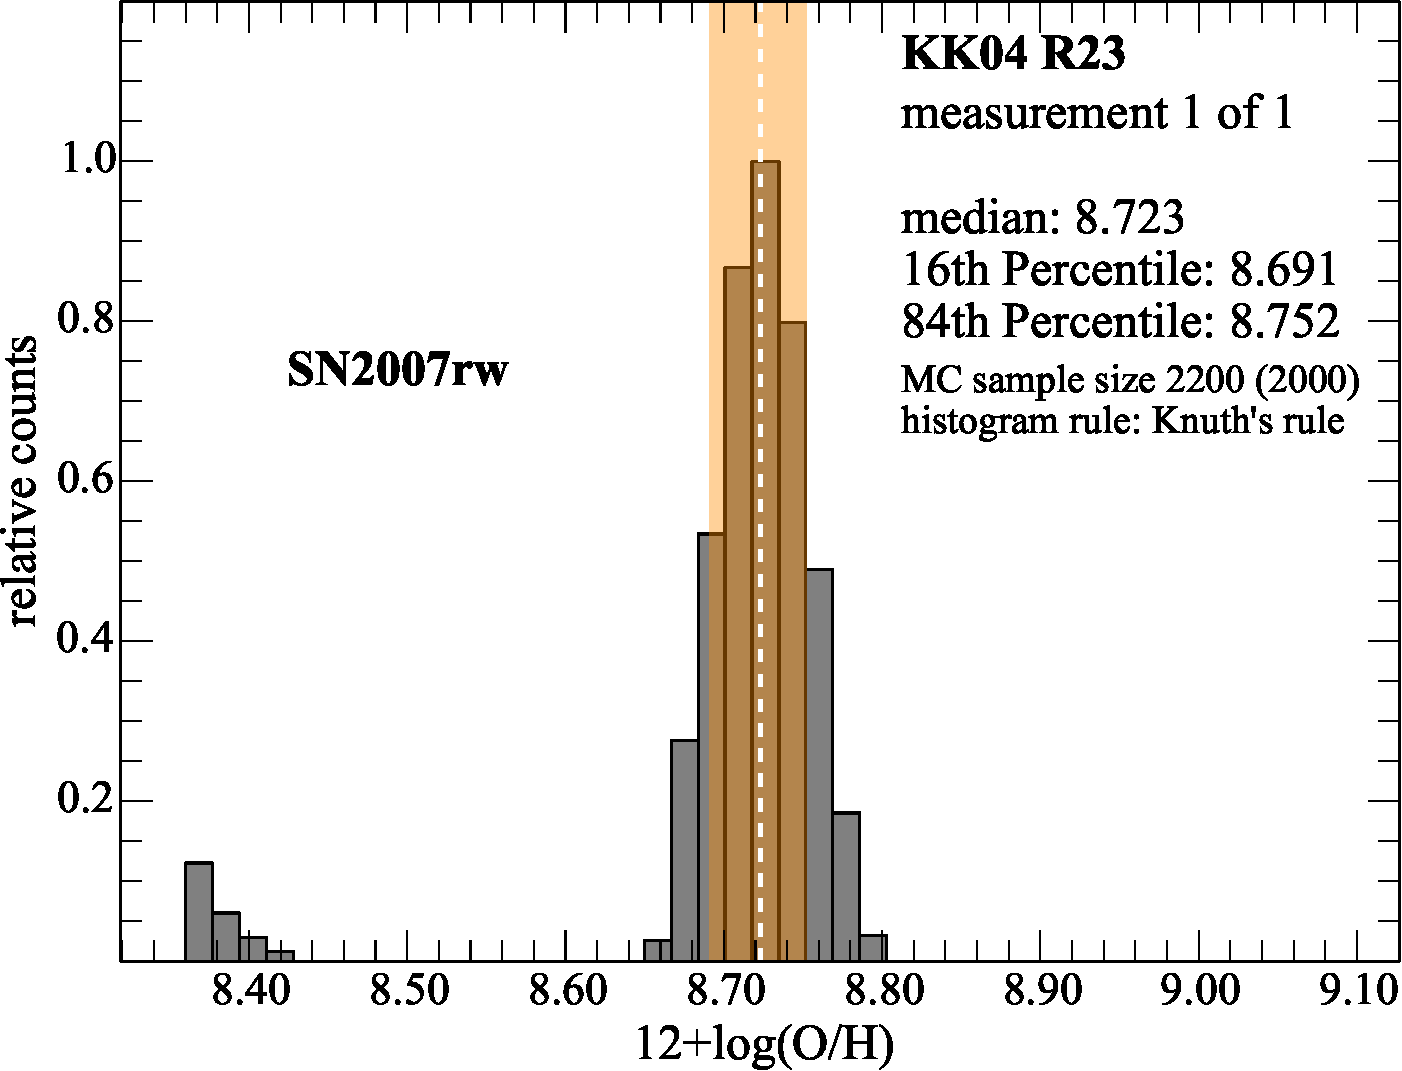
\includegraphics[width=1.0\columnwidth]{SN2007rw_n2000_KK04_R23_1.pdf}
\caption{Metallicity distribution according to the KK04\_$R_{23}$ scale for the site of SN~2007rw, as measured in  \citet{modjaz11}. The $R_{23}$ based scales are double valued: for the same $R_{23}$ value there are two metallicity solutions. The KK04\_$R_{23}$ scale uses the ionization parameter $q$ in an iterative fashion to determine the metallicity by selecting the upper or the lower branch value. In some cases, when the errors in the measurements are large, or for particular flux ratios, the solution may oscillate between the upper and lower branch in different realizations, giving rise to a bimodal metallicity distribution. These cases are easily identifiable by looking at the visual tools the code generates, such as this histogram.}\label{metallicity_bimodal}
\end{figure}

Since the metallicity distributions are not Gaussian, the percentiles we report cannot be expressed in terms of $\sigma$ values. In determining the confidence region for asymmetric and multi-modal distributions, there are broadly three approaches (e.g., \citealt{andrae10}): choosing a symmetric interval, the shortest interval, or a \emph{central} interval.  With the central method we determine the confidence interval by choosing the left and right boundaries such that the region outside the confidence interval on each side contains $16\%$ of the total distribution $-$ in analogy to the one-sigma-interval of a Gaussian distribution. This ensures that the algorithm finds the proper boundaries even for asymmetric, non-Gaussian distributions, and in the case of multiple peaks. In summary, the output for the measured value corresponds to the fiftieth (50\%) percentile, while the lower error bar corresponds to the 50$^{th}$-16$^{th}$ percentile and the upper error bar corresponds to 84$^{th}$-50$^{th}$ of the metallicity estimate distribution. 
%However, we urge the reader to always inspect the metallicity distribution plots, which are also outputted, to check for themselves whether the outputted median and confidence regions properly represent the metallicity distribution (see Section~\ref{vizs})

The distributions for the D02 scale include the uncertainty in the fit parameters: the oxygen abundance in this scale is generated as \oxab~=~$9.12~\pm 0.05 + (0.73~\pm 0.10)\times\mathrm{[NII]}/\mathrm{H}\alpha$ \citep{denicolo02}. The parameters of the fit are generated as the sum of the nominal parameters (9.12 and 0.73) and a Gaussian distributed random value centered on zero, and within a standard deviation of 0.05 and 0.10, respectively, in the above units.
Similarly, the distributions for the M13 scales include the uncertainty in the fit parameters as stated in \citet{marino13}: the oxygen abundance as a function of [NII]/\ha~ is parametrized as \oxab~=~$8.743~\pm 0.027 + (0.462~\pm 0.024)\times\mathrm{NII}/\mathrm{H}\alpha$, and as a function of $\frac{\mathrm{[OIII]/H}\beta} {\mathrm{[NII]/H}\alpha}$ as \oxab~=~$8.533~\pm 0.012 + (0.214~\pm 0.012)\times\frac{\mathrm{[OIII]/H}\beta} {\mathrm{[NII]/H}\alpha}$.

We note that our code does not output the \emph{systematic} uncertainty of each scale, which, for example, is $\sim$0.15 \nolinebreak dex  for KD02. However, if all metallicity measurements are in the \emph{same} scale and only \emph{relative} comparisons are made, as recommended by a number of authors, then the systematic error does not have any impact (by definition!). Nevertheless, it is then necessary to obtain statistical error bars, as computed in the code we are releasing here, for meaningful relative comparisons.

%However, the
%relative metallicity difference measured between a given pair
%of galaxies in different diagnostics is consistent with an rms
%scatter typically ?0.07 dex, and 0.15 dex between the most
%discrepant diagnostics (Kewley&Ellison 2008).


%from Kewley & Ellison08: The cause of the metallicity calibration discrepancies remains unclear. The discrepancy has been attributed to either an unknown problem with the photoionization models (Kennicutt et al. 2003) or temperature gradients or fluctuations that may cause metallicities based on the electron temperature method to underestimate the true metallicities (Stasinska 2002, 2005; Bresolin 2006). Until this discrepancy is resolved, the absolute metallicity scale is uncertain.

\subsubsection{Visual diagnostics}\label{vizs}


\begin{deluxetable*}{lccccccccc} 
%\setlength{\tabcolsep}{0.0001in} 
\tabletypesize{\tiny}
\setlength{\tabcolsep}{0.0000001in} 
\tablecolumns{10}
%%\tablewidth{114.88pt}
\tablecaption{Example Data and their Uncertainties based on Data in \citet{modjaz11}}
\tablehead{   % column headings
  \colhead{site} &
  \colhead{[OII]3727} & 
  \colhead{\hb} & 
  \colhead{[OIII]4959} & 
  \colhead{[OIII]5007} & 
  \colhead{[OI]6300} & 
  \colhead{\ha} & 
  \colhead{[NII]6584} & 
  \colhead{[SII]6717} & 
  \colhead{[SII]6731} 
}
\startdata
08D & 1.842 (.053) &	0.958 (.032) &	NaN          &	0.302 (.029) &	0.127 (.021) &	4.746 (.026) &	1.642 (.022) &	0.941 (.021) &	0.543 (.019) \\
06fo & 2.875 (.101) &	1.251 (.044) &	0.168 (.028) &	0.064 (.025) &	NaN          & 	4.026 (.069) &	0.781 (.033) &	0.821 (.035) &	0.573 (.032) 
\enddata
\label{tab:exampledata}
\end{deluxetable*}

In order for the user to check the validity of a measurement, and to better understand the distribution of metallicity values, we provide two visualizations: for each set of input line fluxes, we generate a histogram of the output distribution in all metallicity scales calculated (Figures \ref{metallicity_distribution}, \ref{metallicity_bimodal}, and \ref{fig:KDE}), and for each set of input line fluxes we generate a \emph{box-and-whiskers} plot (hereafter \emph{boxplot}, for short) summarizing the result of all scales calculated (Figure \ref{boxplot}). All the plots generated by are code are created with Python \verb=matplotlib= \citep{hunter07}.

Choosing the binning size for a histogram is not a trivial task.  \citet{hogg08} describes various data analysis recipes for selecting a histogram bin size. Too many bins will result in an ``over-fit'' histogram, while too few bins may miss features of the distribution. 
By default, we use \emph{Knuth's Method} to choose the number of bins $N_\mathrm{bins}$ for each histogram. Knuth's method  optimizes a Bayesian fitness function across fixed-width bins \citep{knuth06}. Additionally, however, we enable a number of binning options from which the user can choose, including: 
the square root of the number of points, $N_\mathrm{bins}=\sqrt{N}$, \emph{Rice rule} ($N_\mathrm{bins}~=~2\sqrt[3]{N}$, e.g., \citealt{hastie09}), 
\emph{Doane's formula} ($N_\mathrm{bins}~=~1 + \mathrm{log}_2{N} + \mathrm{log}_2\left(1 + \mathrm{Kurt}\sqrt{(N / 6)}\right)$, where Kurt is the third moment of the distribution, \citealt{doane76}\footnote{\citet{doane76} attempted to address the issue of finding the proper number of bins for the histogram of a skewed distribution. Several versions of the so-called Doane's formula exist in the literature. Our formula can be found, for example, in \citealt{bonate11}}), and the full Bayesian solution, known as Bayesian Blocks, which optimizes a fitness function across an arbitrary configuration of bins, such that the bins are of variable size \citep{scargle13}. The implementation of the latter method requires the \verb=astroML= Python package to be installed on the user's system (\citealt{astroml}\footnote{\url{https://github.com/astroML/astroML}}). If the \verb=astroML= package is not found, the code will default to Knuth's Rule. 
As mentioned, Knuth's method implies an optimization. In cases in which the convergence takes too long (or if the number of bins after the minimization is  $N_\mathrm{bins}/\sqrt{N} > 5$ or $N_\mathrm{bins}/\sqrt{N} < 1/3$) the code will revert to Rice rule.
Some methods may be computationally prohibitive with a very large sample size, or very little computational power, such as the Bayesian methods that rely on optimization (Knuth's method and the Bayesian Block method) in which case it may be convenient for a user to choose Doane's formula, Rice rule, or even the square root of the number of samples. 

\begin{figure}[ht!]
%  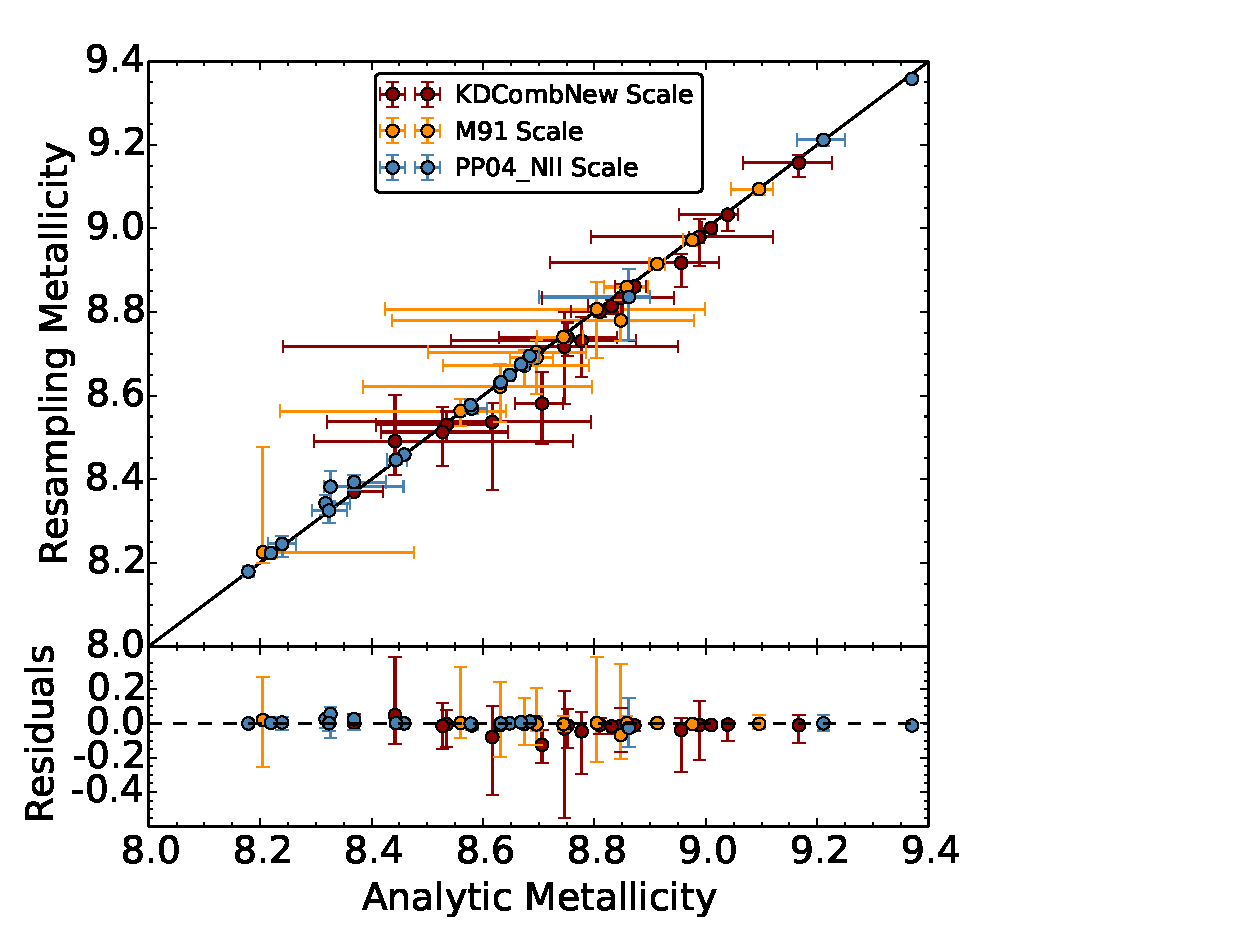
\includegraphics[trim = 10mm 0mm 10mm 0mm, clip]{abcomparison6.eps}
  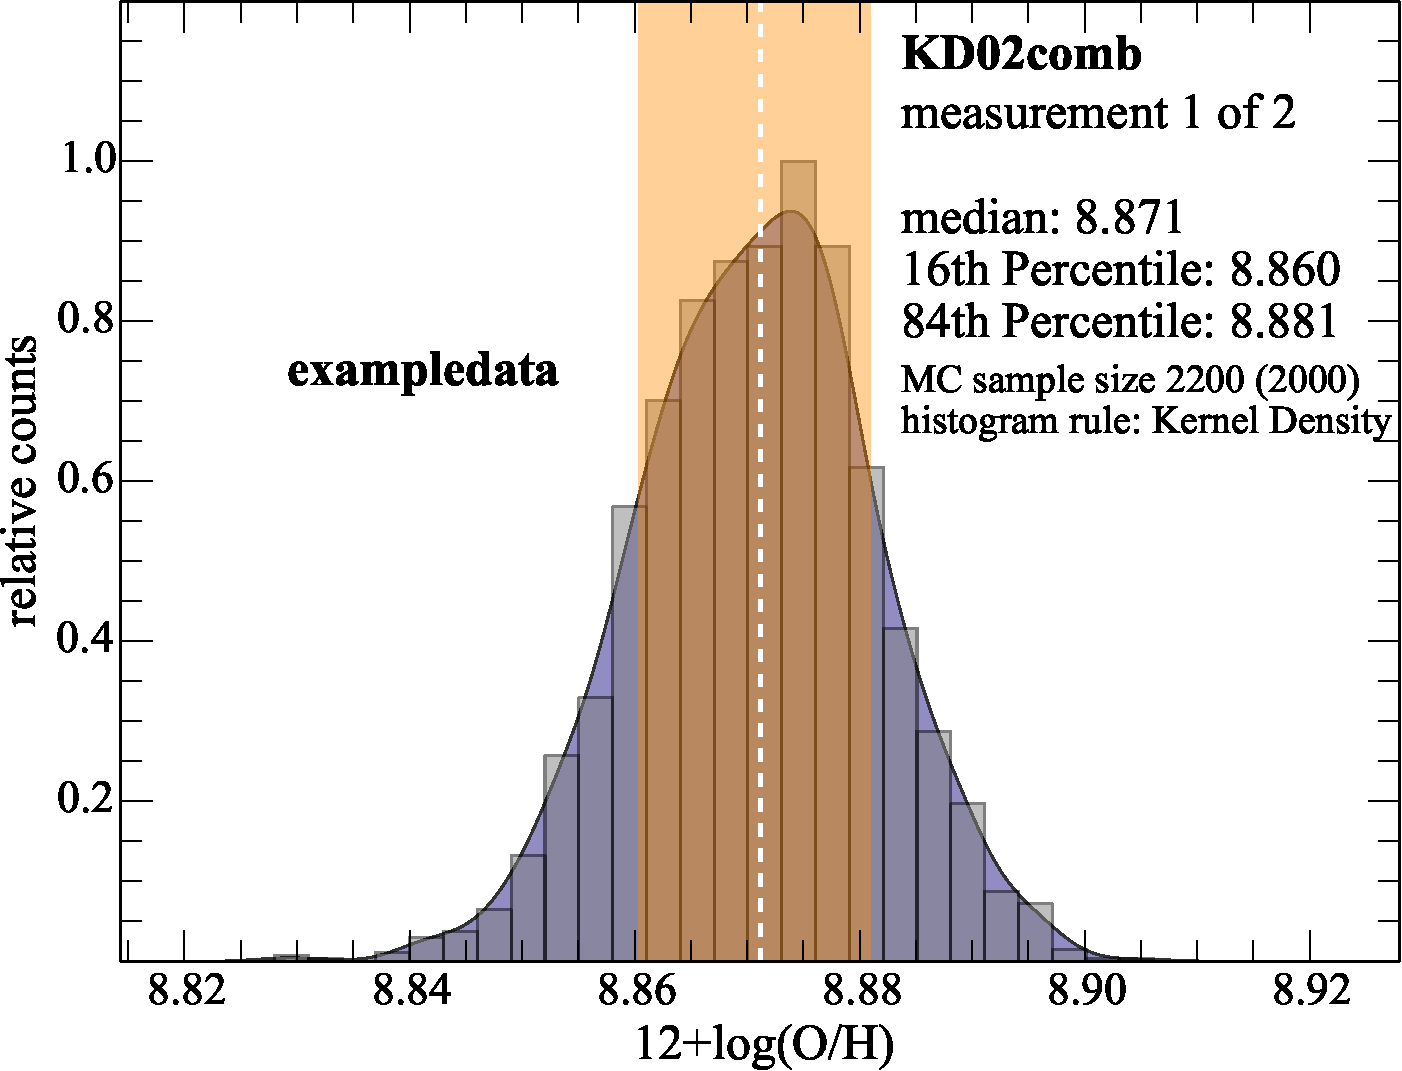
\includegraphics[width=1.0\columnwidth]{exampledata_n2000_KD02comb_1KDE.pdf}
   \caption{The Kernel Density for the distribution of values for the KD02comb scale, as described in \citet{kewley08}, for the first measurement of our example data (Table~\ref{tab:exampledata}) is plotted. The Kernel density is displays as a blue shaded region, and it is calculated via \emph{KD Tree} with a gaussian kernel with bandwidth given by Silverman's rule as described in Section\ref{vizs}, and normalized as described in the same Section. The histogram of the distribution with min size chosen according to Knuth's rule is over-plotted (gray bins) and the median and confidence intervals are shown as described in Figure~\ref{metallicity_distribution}.}\label{fig:KDE}

\end{figure}
Lastly, the user can generate and visualize the metallicity distribution \emph{Kernel Density} if the \verb=sklearn= package is installed. Kernel Density Estimation (KDE) alleviates the problem of choosing the bin size, at the cost of specifying a convolution kernel. The Kernel Density of the distribution is here calculated via \emph{KD Tree} with a gaussian kernel, as explained in the \verb=sklearn= package documentation\footnote{\url{http://scikit-learn.org/stable/modules/density.html}}. The bandwidth of the kernel is chosen accordingly to \emph{Silverman's rule} \citep{silverman86}\footnote{By Silverman's rule the bandwidth for the KDE kernel is set to $w~=~1.06\sigma~N^{-0.2}$, where $\sigma$ is the sample standard deviation. Although the bandwidth chosen accordingly to Silverman's rule is only optimal in the case of a Gaussian basis and a Gaussian distribution, and our distributions are explicitly \emph{not} Gaussian, as explained earlier, this kernel parametrization generally provides good results for our metallicity distributions.}. The results will then show both a histogram, with $N_\mathrm{bins}$ chosen via Knuth's method, as well as the distribution Kernel Density, as shown in Figure~\ref{fig:KDE}. The KDE is saved as binary (\verb=pickle=) python object (an \verb=sklearn= \verb=KernelDensity= object), so that it can be recovered outside the code and used as a probability distribution for further inference.

The histograms are always normalized so that the highest bin value is 1, and the  Kernel Density is normalize to contain the same area as the overplotted histogram. 


\begin{figure}[ht!]
%  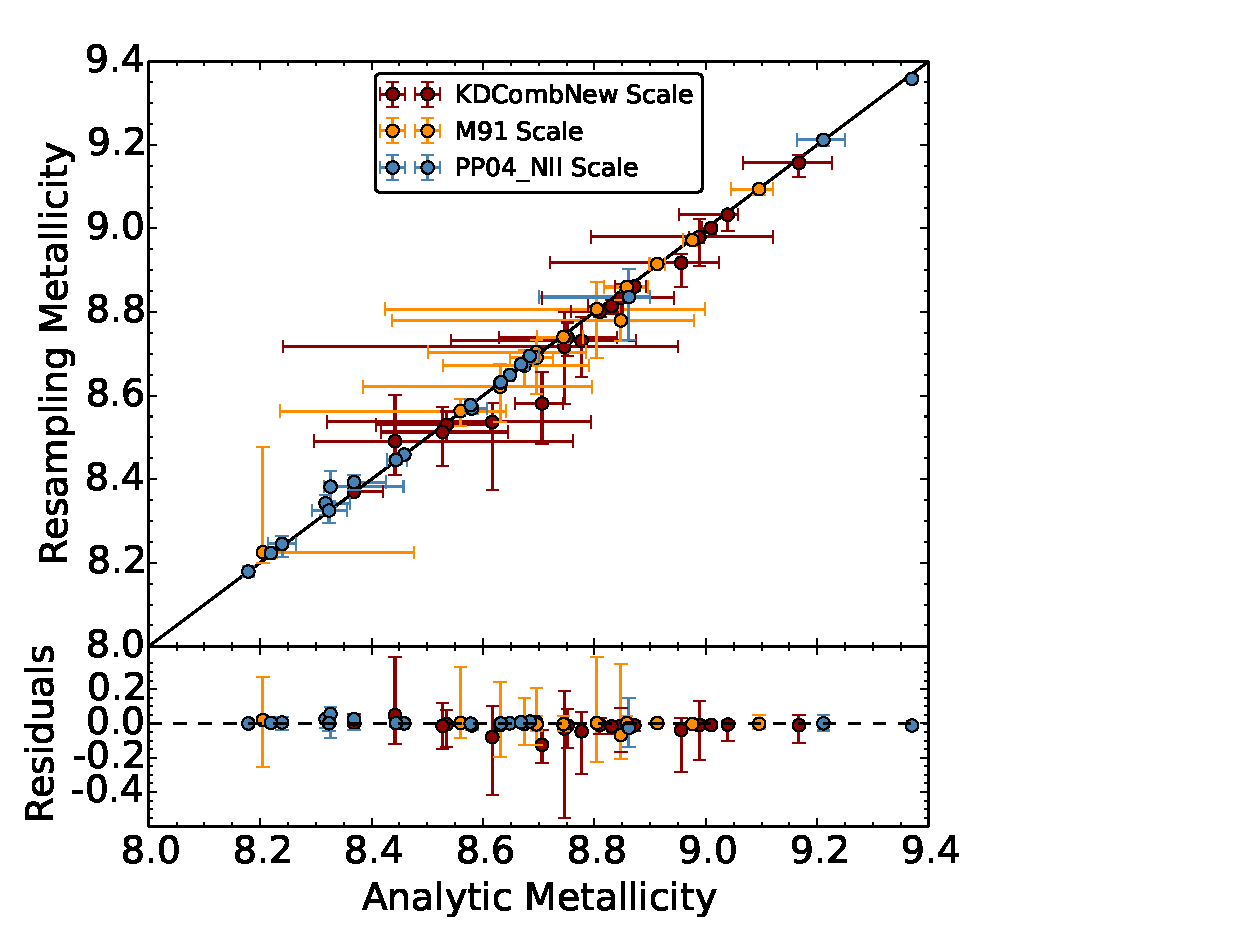
\includegraphics[trim = 10mm 0mm 10mm 0mm, clip]{abcomparison6.eps}
  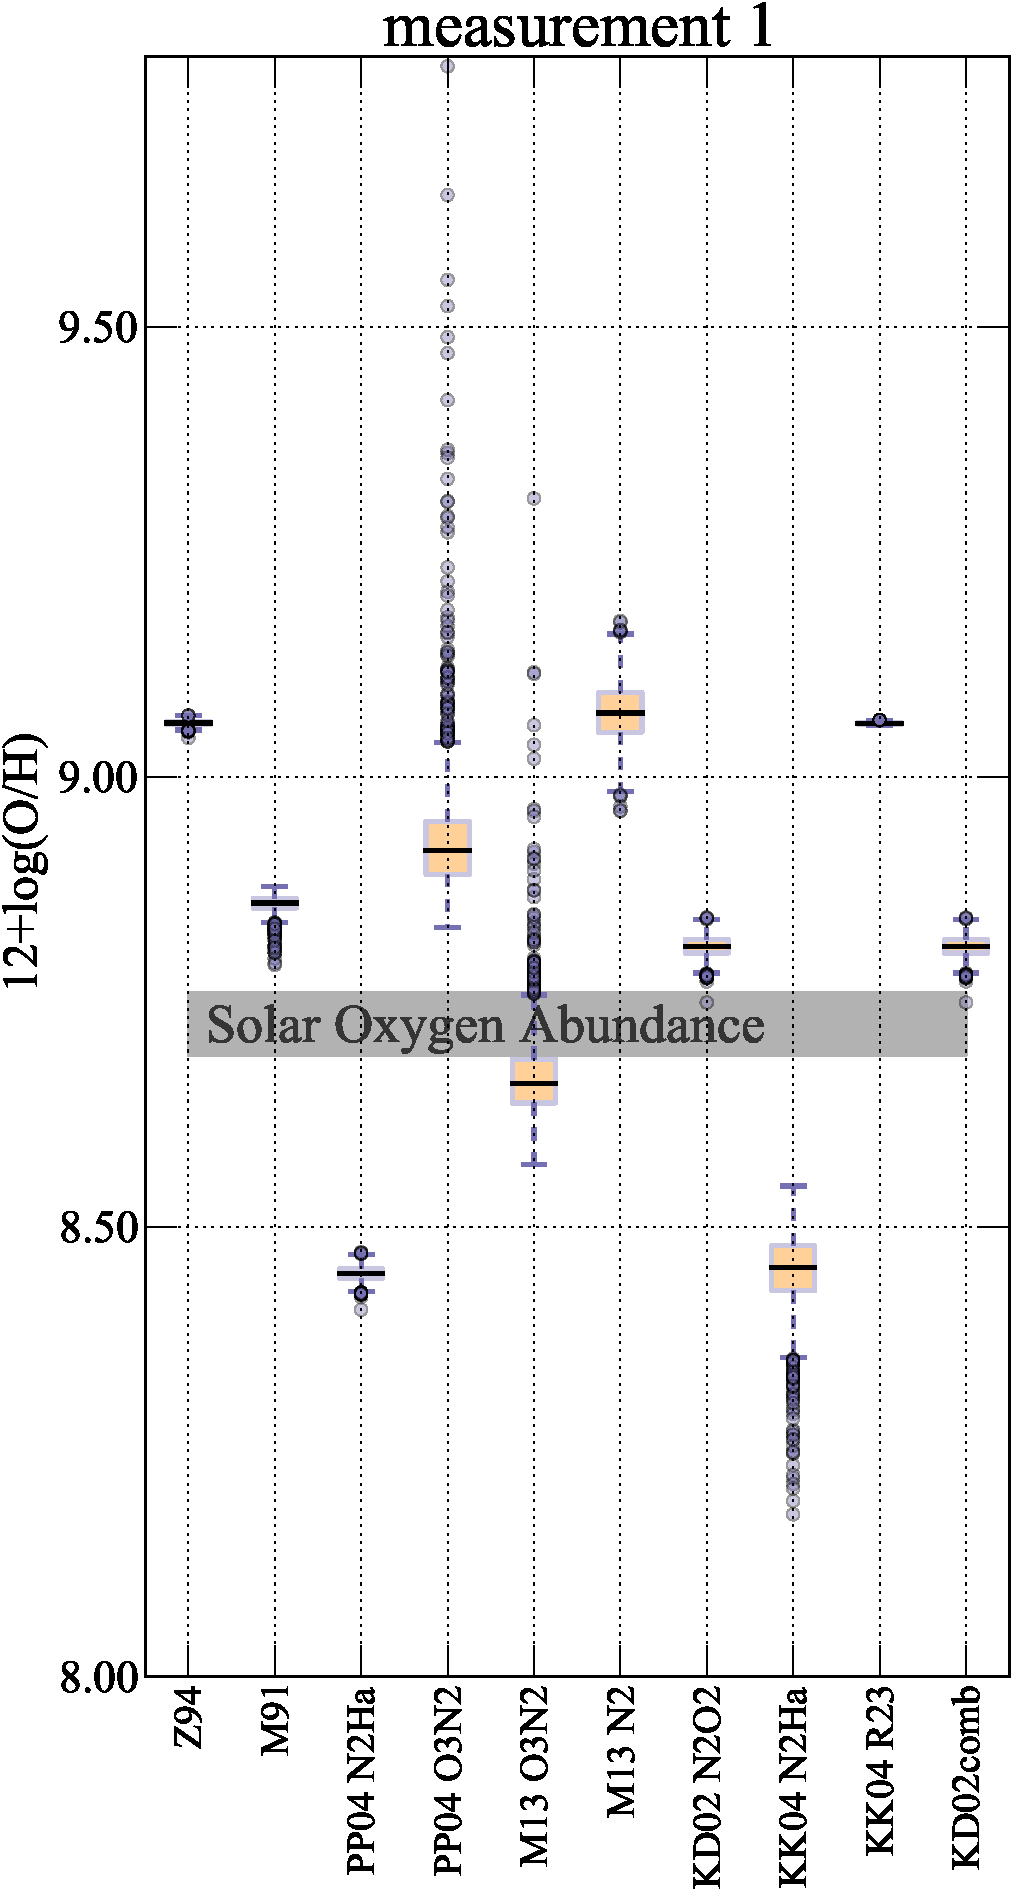
\includegraphics[width=0.95\columnwidth]{exampledata_boxplot2000_m1.pdf}
   \caption{A box-and-whiskers plot shows the comparison of the results of 11 metallicity calculations, corresponding to 5 scales as listed above, calculated from the same set of measured lines (Table~\ref{tab:exampledata}, host galaxy of SN~2008D). For each scale, the median of the resulting distribution is plotted as a horizontal line, the inter quartile range (IQR) is represented as an orange box, and the bars, joined to each end of the box by a dashed line, represent the minimum and maximum of the distribution \emph{excluding outliers}, where outliers are defined as any point farther than $1.5\times$ IQR from the edges for the IQR.}
 \label{boxplot}
\end{figure}

At each run the code also generated a boxplot (Figure~\ref{boxplot}). The boxplot summarizes the result from each scale the user chooses to calculate. For each scale the median of the \oxab~ distribution is plotted as a black horizontal line. The height of the corresponding box represents the $25^{th}$ percentile of the \oxab~ distribution, known as the \emph{interquartile range} (IQR). 
The bars represent the maximum and minimum value of the distribution, excluding outliers. The outliers are plotted as circles, and are defined as all data points farther than $1.5\times\mathrm{IQR}$ from the $25^{th}$ percentile (i.e. from either end of the box). 

%MM:  also do you have a reference for defining outliers this way?
%%FED: no, it is how it is just the standard for boxplots,
The Solar oxygen abundance is indicated in this plot for comparison: a gray box shows a range of estimated values for Solar oxygen abundances, from \oxab=8.69 \citep{asplund09_rev} to \oxab=8.76 \citep{chaffau11}.
Notice that only the diagnostics requested by the user have a slot in the plot (in the example in Figure~\ref{fig:KDE} the computed scales are Z94, M91, the PP04, the M13, and the KD02 scales). However these slot exists on the plot whether the diagnostic can be produced or not, i.e. if the set of input lines does not allow a requested scale to be calculated an empty column will be generated in this plot in correspondence of said metallicity scale. 

With this plot the user can immediately check for consistency or scatter in the metallicities derived by the requested scales (e.g., there are well-known systematic offsets between different methods, where the $T_e$-based, empirical methods usually give lower values than the photoionization based ones), and coarsely assess the shape of the distribution in each scale (e.g. strong asymmetry or bimodality would show up as an asymmetric box, or a very asymmetric distribution of outliers).



\subsection{Visual diagnostic to assure completeness of the MC simulation}\label{sec:completeness}

\begin{figure*}[!ht]
%\epsscale{0.6}
\centerline{
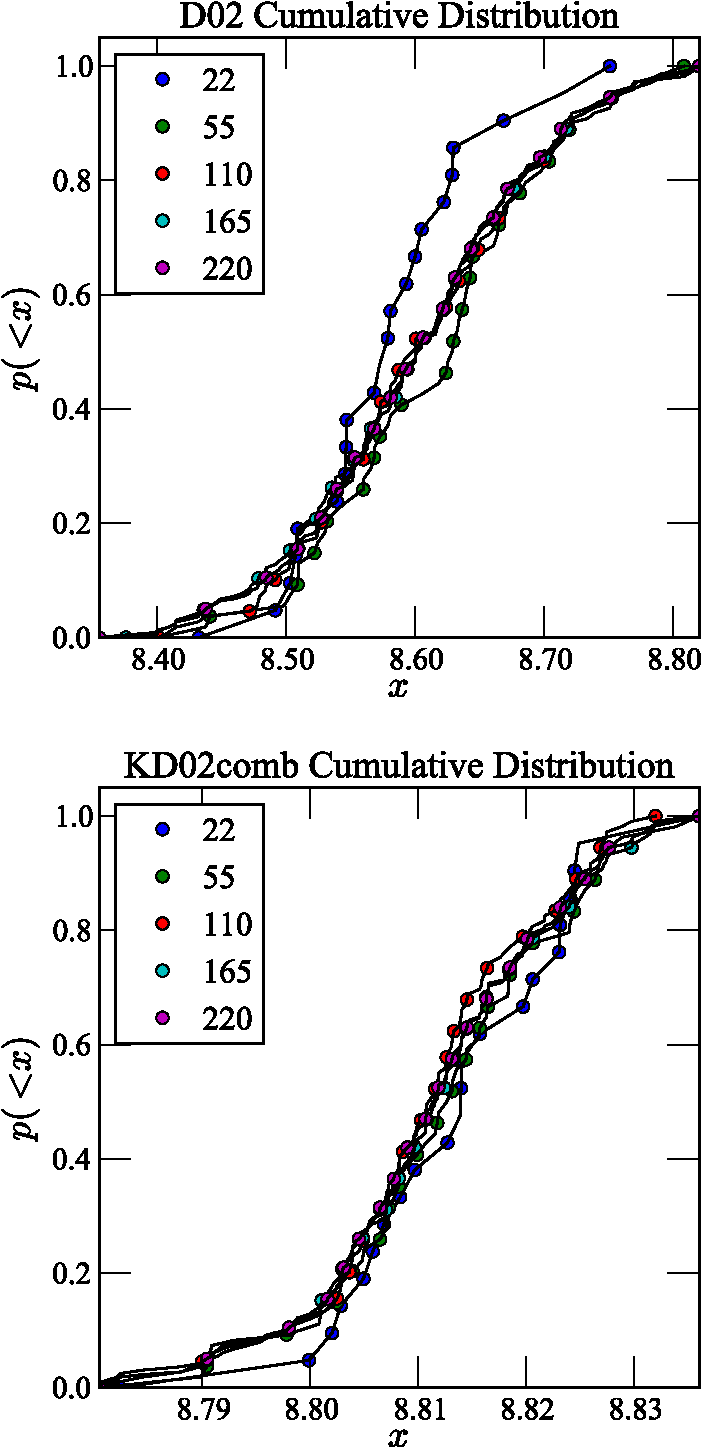
\includegraphics[width=0.65\columnwidth]{exampledata_n200_testcomplete.pdf}
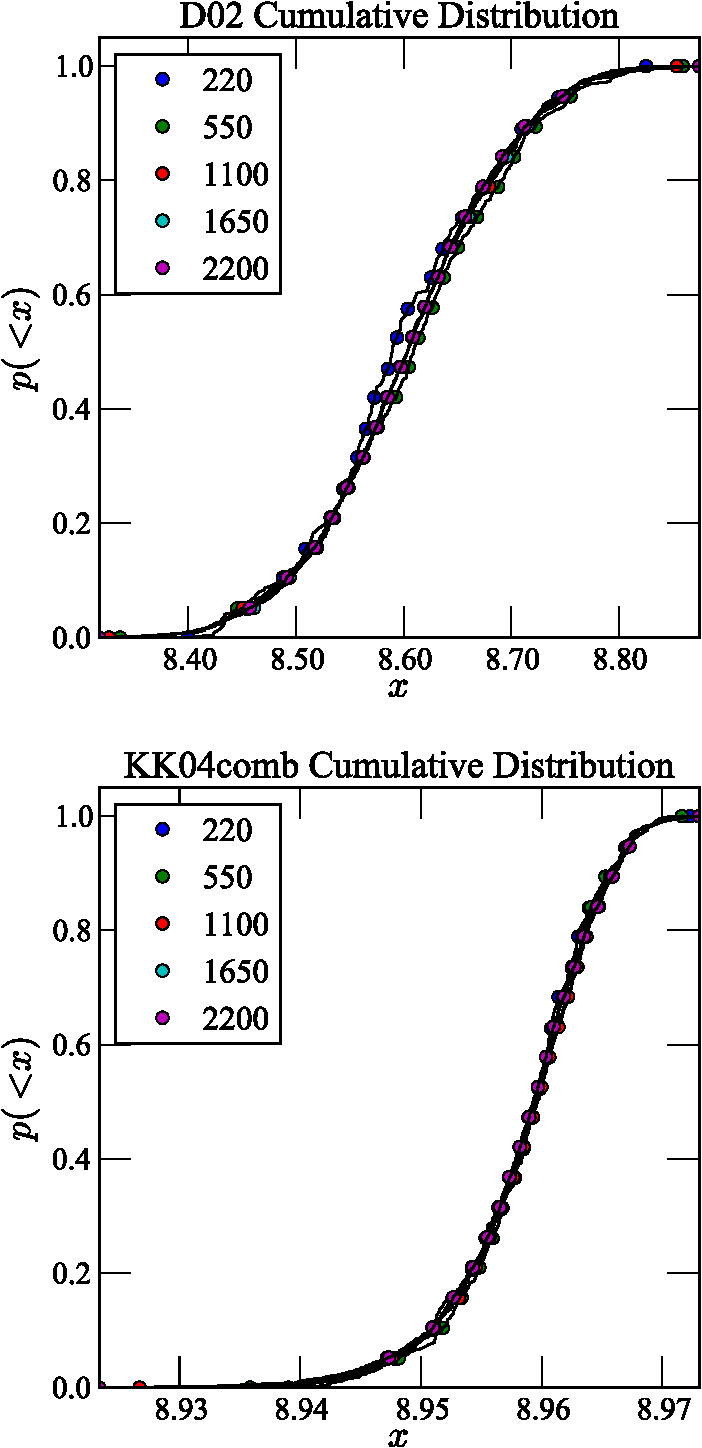
\includegraphics[width=0.65\columnwidth]{exampledata_n2000_testcomplete.pdf}
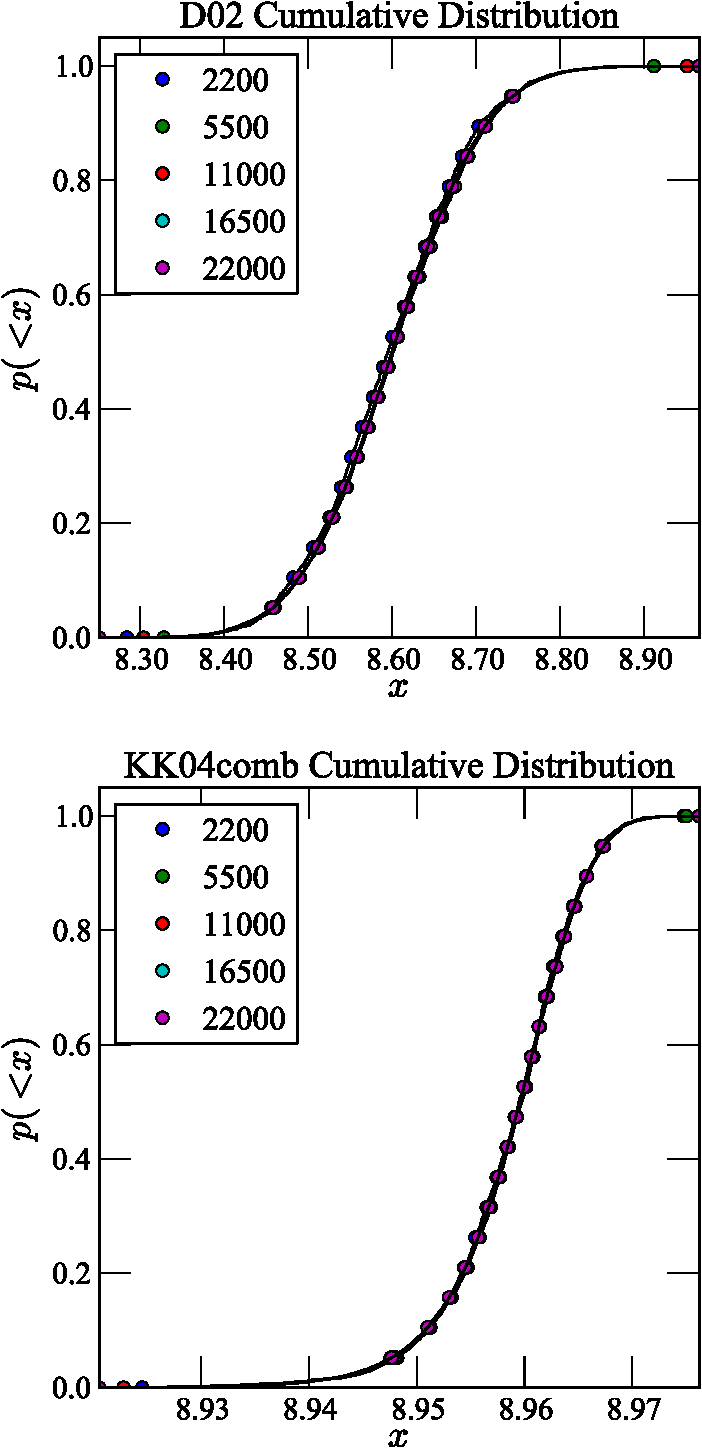
\includegraphics[width=0.65\columnwidth]{exampledata_n20000_testcomplete.pdf}}
% exampledata_n50000_M91_1.ps}
%\vspace{0.2in}
\caption{Cumulative plots of the distribution of metallicity values for the D02 \citep{denicolo02} and KD02 scale (\citealt{kewley02}, updated by \citealt{kewley08}), chosen here just as examples, where $x$ refers to \oxab. The input used is example data 1, the emission line values for the host galaxy of SN~2008D from \citet{modjaz11}. In each plot the cumulative distribution is shown for a randomly chosen subsample of 10\% of the data in the sample, as well as a subsample of 25\%, 50\%, and 75\%, of the data, and for all data in the distribution. In the left plots the distributions are generated from an $N=200$ samples, in the center top and bottom plots from an $N=2,000$  and in the right-most column from a $N=20,000$ sample. The increasing overlap of the distributions informs us about completeness. In the left plots the distributions do not fully overlap, indicating that completeness is not achieved with the $N=200$ sample. On the other end, since all subsamples are indistinguishable in the top and bottom plots on the right, which are generated with $N=20,000$ samples, we conclude that completeness is already achieved at 10\% of the $N=20,000$ sample (the smallest sample in the plots on the right) for our example data, i.e. , at $N=2,000$ which we use for the rest of this work.}
 \label{cd}
%\end{center}
%\vspace{-0.5in}
\end{figure*}

The user chooses $N$, the number of samples to be generated.  Note that the final sample size is 10\% larger than the user chosen parameter $N$. The sample size is in fact automatically increased by 10\% at the beginning of the run, in order to assure that even if during the calculations some of the output metallicities were to result in non-valid values (\emph{NaN}'s or infinities, for example, if devision by very small numbers is required) the actual sample size is at least as large as the user intended. With reasonable input parameters, the code rarely produces non-valid values, and if the size of the valid output distribution were in the end smaller than the \emph{requested} value $N$, i.e. if the number of non-valid outputs is larger than 10\% of $N$, the user should in fact worry about the set of input line fluxes used. 

Of course the reliability of the metallicity estimates depends crucially on the sample size being sufficiently large to properly characterize the distribution of metallicity values. It is however not trivial to decide when $N$ is sufficiently large. As soon as $N$ is large enough, and the distribution is well characterized, adding more synthetic data will not change its shape. Consider a cumulative distribution for a metallicity scale, D02, for example, which has noise from the measurement errors, as well as from the error in the fit parameters, or KD02, which uses a non linear combination of the input line flux values. We plot the cumulative distribution for four randomly selected subsamples of the data points in the distribution, of size 10\%, 25\%, 50\%, 75\% of $N$, as well as for the entire distribution. If 1/10th of the points were a sufficiently large Monte Carlo sample, the cumulative distributions would typically appear smooth and, most importantly, they would overlap. In Figure~\ref{cd} we show these cumulative plots for a distribution generated with $N=200$, $N=2,000$, and $N=20,000$, for D02 and KD02comb.

The cumulative distributions for the subsets of the $N=200$ simulation (left panel in Figure~\ref{cd}) are different, and noisy, indicating that 200 data points is not a sufficiently large dataset. Conversely, at $N=20,000$ (right panel) the distributions are indistinguishable, indicating that $N=2,000$ (the smaller subset in this panel) is large enough. The $N=2,000$ cumulative distributions rapidly converge, as the subsample size increases, indicating that a value of $N$ between 200 and 2,000 will characterize the distribution appropriately for our example data set.  In the light of this we choose, conservatively, $N=2,000$ to run our simulations for this dataset. 

We remind the user that the appropriate number of $N$ samples will depend on the diagnostic, and on the input data. The errors on the measurements, and the calculations performed to derive the metallicity from line ratios, which are for many scales non-linear, will determine the shape of the distribution, and thus the number of data points that are needed to fully characterize it. 

\subsection{Performance and Benchmarks}
We ran a bench mark calculation on a MacBook Air with a dual-core Intel Core i7 (1.7~GHz) and 8GB of 1600 MHz DDR3 memory. The dataset we used for the calculation includes 2 sets of line measurements (measurement 1, the host galaxy of SN~2008D, and measurement 2, the host galaxy of SN~2006fo). The flux values and their associated errors are shown in Table~\ref{tab:exampledata}. The code performs simple algebraic operations on large data arrays. It is vectorized along the sample-size dimension, so that the code loops over the smaller dimension corresponding to the number of sets of line measurements in input (2 in our example data), while operations are generally performed on the $N$-dimensional vectors storing the synthetic measurements, and the $N$-dimensional variables hence derived (certain scales, such as the KD02 and KK04 ones, derive the ionization parameter in an iterative fashion requiring further loops).


With full graphic output (all histograms are being plotted) and performing all default metallicity calculations, except those of D13 \emph{pyqz}, for our example data sets and a sample size $N=2,000$, the time required by the code is $\sim14.5$ seconds (wall clock time, and less then half a second longer in total CPU time, recall that the machine we tested on is dual-core), and less then 0.3 seconds of CPU time spent in the kernel within the process. Including  the scales of D13 \emph{pyqz} for the same datasets, the run time becomes $\sim29$ seconds of clock time (and actual CPU time). 
The code time was tested on sets of 1, 2, 5, 10, 25, 50 and 100 identical measurements (copies of the emission line fluxes of  the SN~2008D host galaxy in our example dataset) and the clock time is found to scale roughly quadratically with the number of measurements in input, but with a small quadratic coefficient $\sim0.07$, and with linear coefficient $\sim7$. This means effectively that the 100 measurements sample will take 200 times longer than the 1 measurement sample (of course with dependence on which lines are available in each measurement). For the CPU time spent in the kernel we find a roughly linear relation with the number of input measurements, with a very shallow dependency of $\sim 0.05$. This is the actual computational time in calculations performed in the code: most clock time is in fact spent in root finding, input-output, and plotting activities.

% FED: I still have an inconsistency between the time in the plot and in the timing tests. I will resolve it ASAP.

The time spent on plotting functions, which includes the calculation of the appropriate number of bins for each scale, is substantial: 1.67 seconds per distribution on average with 14 calls for this data set (one for each metallicity scale, E(B-V), and $R_{23}$). 
%In Table~\ref{tab:time}  we summarize the time spent on each metallicity scale for SN~2008D, the first measurement of the sample dataset, for each metallicity scale, and 
We summarize the run time spent on each metallicity scale and memory usage for the host galaxy of SN~2008D, the first measurement of the sample dataset, in Figure~\ref{fig:mem}. While the CPU usage is modest, the memory usage can be large, depending on the size of the sample.  The memory usage ramps up quickly, as soon as the $N$ line samples are created, 
and remains fairly constant throughout the run.  Figure~\ref{fig:mem} shows the memory used by each function in the code as a function of time for a single set of input lines of our example data (host galaxy of SN~2008D). The scales that take longer time require the root finding (e.g. M08), or optimizations which are done iteratively (e.g. KD02\_N2O2).

\begin{figure}[ht!]
%  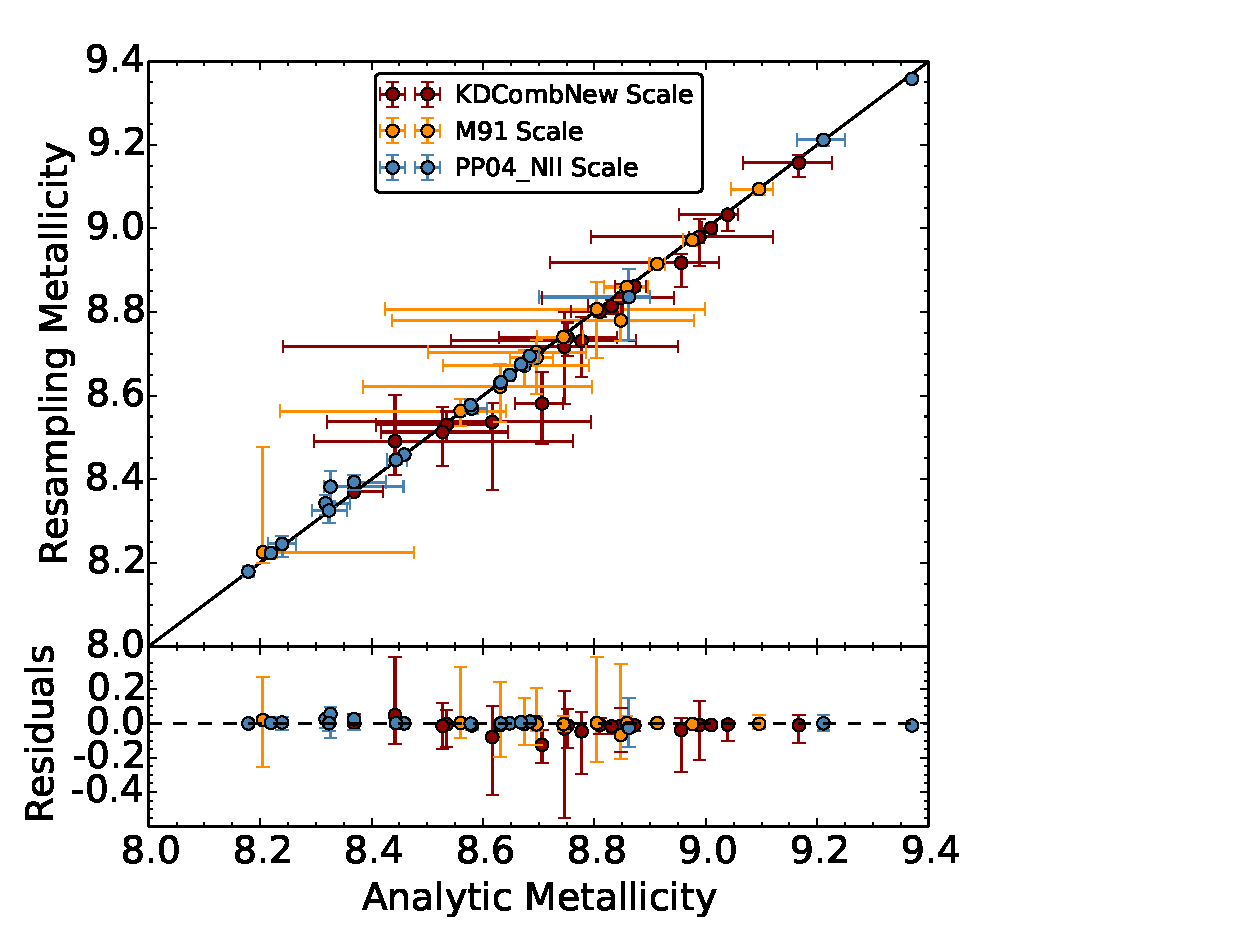
\includegraphics[trim = 10mm 0mm 10mm 0mm, clip]{abcomparison6.eps}
  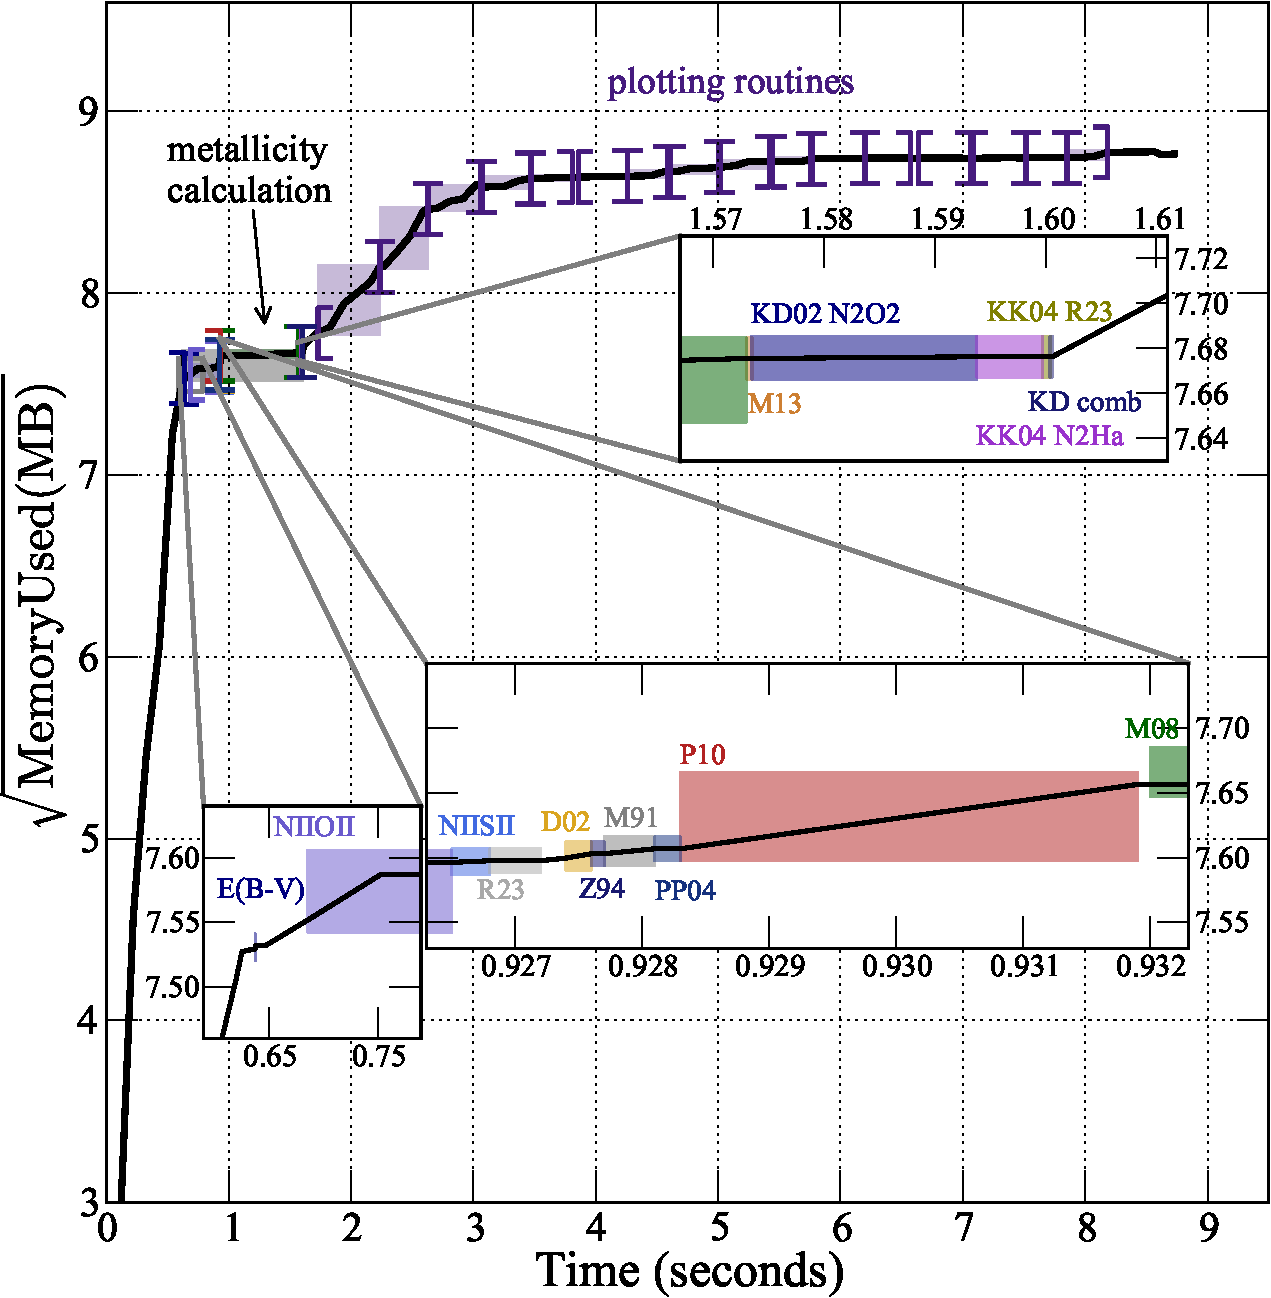
\includegraphics[width=1.0\columnwidth]{memusage.pdf}
   \caption{Memory usage: we plot the square root of the memory usage in Megabytes as a function of time for running our code (using $N$=2,000 and all default metallicity scales except the D13 \emph{pyqz} ones) on a single set of measured emission lines (Table~\ref{tab:exampledata}, host galaxy of SN~2008D). The square root is plotted, instead of the natural value, to enhance visibility.  
Three inserts show zoom-ins of the region where most of the metallicity scales are calculated, since the run time of the code is dominated after all scales are computed, by plotting routines, including the calculation of the bin size with Knuth's rule. 
Each function call is represented by an opening and closing bracket in the main plot, and by a shaded rectangle in the zoom-in inserts.
%%MM: For the labeling: NIIOII NIISII and R23 - these are not specific scales but just ratios, right?
%FED: that's correct, but i dont think i say they are strictly ``scales'' anywhere
The calculation of NIIOII, which requires 0.26 seconds (update in the end), is split between two inserts, as well as the calculation of the M08 scales (three scales) which require 0.78 seconds. Altogether, the calculation of metallicity in all scales, except those in the D13 \emph{pyqz} scales, takes 1.15 seconds. For technical details about the D13 \emph{pyqz} scales performance we refer the reader to the \emph{pyqz} package. FIX WITH FINAL VERSION OF PLOT}
 \label{fig:mem}
\end{figure}



%\begin{deluxetable}{lr} 
%%\setlength{\tabcolsep}{0.0001in} 
%\tabletypesize{\tiny}
%\setlength{\tabcolsep}{0.001in} 
%\tablecolumns{2}
%%%\tablewidth{114.88pt}
%\tablecaption{CPU usage by scale}
%\tablehead{   % column headings
%  \colhead{Scale} &
%  \colhead{Time ($\times 10^{-6}$ sec)} 
%}
%\startdata
%E(B-V)    &   100.1     \\ 
%$R_{23}$   &   599.9     \\ 
%M91       &   600.1      \\ 
%Z94       &   100.1       \\
%%C01       &        \\ 
%P05       &   399.8     \\ 
%D02       &   300.2     \\ 
%PP04      &   200.0     \\ 
%M08       & 1.720$\times 10^6$ \\
%P10       &  5300 \\
%M13       &   500.0 \\
%pyqz      &   1.127$\times 10^6$  \\ 
%KK04 $R_{23}$   & 4500    \\ 
%KD02 N2O2 &    500.2     \\ 
%KD02 N2Ha &   3200    \\ 
%KD02\_comb  &   2800 \\
%%diags.initialguess()          &      118.0    \\ 
%%   diags.calcNIISII()             &     254.0    \\ 
%%8497.5        diags.setNII(raw_lines['[NII]6584'])
%%  17077.5        diags.setHab(raw_lines['Ha'],raw_lines['Hb'])
%%  25457.0        diags.setOlines(raw_lines['[OII]3727'], raw_lines['[OIII]5007%'], raw_lines['[OI]6300'], raw_lines['[OIII]4959'])
%%  30478.5        diags.setSII(raw_lines['[SII]6717'],raw_lines['[SII]6731'],ra%w_lines['[SIII]9069'],raw_lines['[SIII]9532'])
%% %378698.0        diags.calcNIIOII()
%\enddata
%\label{tab:time}
%\end{deluxetable}



 
The code is trivially parallelizable, as each measurement can be computed on a different core. Multithreading is enabled via the \verb=multiprocessing= Python module, and when enabled it uses up the $n-1$ codes, where $n$ is the total number of available cores to the user (or less, if a smaller maximum number of cores is set by the user via the global variable MAXPROCESSES).



\subsection{Availability}
The source code is published under MIT-license\footnote{\url{https://github.com/nyusngroup/MC_Metallicity/blob/master/LICENSE.txt}} on GitHub\footnote{\url{https://github.com/nyusngroup/MC_Metallicity}}. At this time the code is released under DOI {\b NUMBER HERE} as version 1.0: {\b NAME HERE}. Project
details, step-wise tutorials, and further information can be found in the module README\footnote{\url{https://github.com/nyusngroup/MC_Metallicity/blob/master/README.md}}.
Development is done in Linux and OS X. The package requires standard python packages, such as \verb=numpy=, \verb=scipy=, \verb=pylab=, and additional features are enabled if the packages \verb=astroml=, \verb=skitlearn=, and \verb=pyqz= are installed, but these packages are \emph{not} required. Contact the authors to be included in a mailing list and be notified about critical changes. 




\section{Comparison to prior uncertainty computation and other works }\label{comp_sec}


A previous method for determining the uncertainty in the oxygen abundance (as used in \citealt{modjaz08_Z,kewley10,rupke10,modjaz11}) was an \emph{analytic} approach of propagating the emission-line flux uncertainties: it found the maximum and minimum abundances via minimizing and maximizing the line ratios by adding/subtracting to the measured line flux values their uncertainties. For comparison we computed the metallicities and their errors in both ways (analytically and using our current MC resampling method) for 3 representative scales. We plot our results and the residuals in Figure~\ref{comp_anal_MC}, which shows a number of important points: i) The metallicity reported as the $50^{th}$ percentile of the metallicity parameter distribution from the MC resampling method is completely consistent with the analytically derived metallicity (i.e., \textbf{DAVID, please fill in} with XXX, XXX and XXX dex for the standard deviation of the residuals for the KD02-comb, M91 and PP04-O3N2 scales, respectively ) -  well within the respective error bars - and thus, the prior published results still stand (unsurprisingly, since our code, aside for the calculation of the confidence interval, uses the same algorithms developed for IDLKD02).
%FED: we need to state the differences here!!%%
%MM: OK - see text for the numbers that David can fill in
 ii) The MC resampling method has smaller error bars than the analytic method, especially for the scales of M91 and KD02. This is easily understandable, since the analytic method assumes the worst-case-scenarios, as it basically yields 2 metallicity parameter draws (the ``minimum'' and ``maximum'') which are in the tail of the full metallicity probability distribution. The MC resampling method is a more correct method as it empirically characterizes the full parameter estimation distribution.
%assumes that \textbf{all} emission line measurement have been drawn from the 68\% tail of the error distribution and 

\begin{figure}[ht!]
  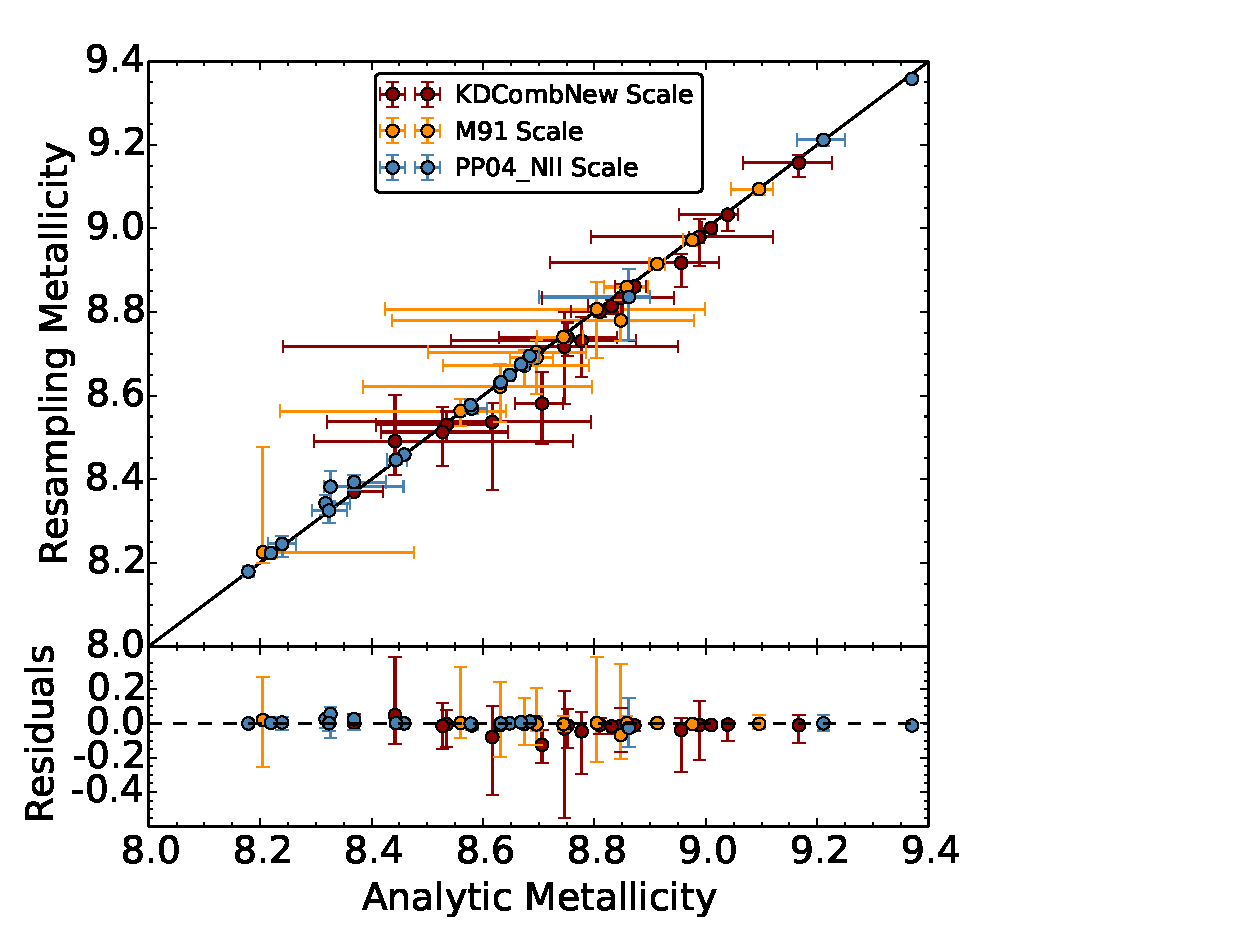
\includegraphics[width=1.0\columnwidth]{abcomparison6.eps}
   \caption{Comparison of metallicity estimation between the analytic method and our Monte Carlo resampling method (top) and their residuals (bottom) for three different metallicity scales. Flux measurements come from 19 galaxies previously measured in \citet{modjaz11}. To add asymmetric errors in quadrature we use $\mathrm{residual}_{\rm min}=\sqrt {x_{\rm max}^2 + y_{\rm min}^2}$ and $\mathrm{residual}_{\rm max}=\sqrt {x_{\rm min}^2 + y_{\rm max}^2}$. Note that for the scales of KD02\_comb and M91,  the MC resampling error bars are smaller than those of the analytic propagation, which assumes worst-case scenarios, while metallicity reported as the 50th percentile of the metallicity parameter distribution from the MC resampling method is completely consistent with the analytically derived metallicity in all scales.}
 \label{comp_anal_MC}
\end{figure}




%Rupke: Errors were propagated primarily using analytic expressions, but for abundance and gradient errors we employed Monte Carlo methods.

\subsection{Comparison with other works}

%Here we perform a literature review of both 


The field of SN host metallicity studies has been rapidly developing as these kinds of studies may be crucial avenues for constraining the progenitor systems of different kinds of explosions - however, a few of the works in this field do not compute errors and others do not show how they compute their statistical errors  (e.g., \citealt{anderson10,leloudas11,sanders12,leloudas14}). %While \citet{sanders12} compute the line flux errors from a Markov-Chain Monte Carlo fitting of a gaussian to the emission lines, they only mention in passing that they propagate the line flux uncertainties into the metallicity measurements, but do not describe how {\bf this is a little harsh, right? i think mentioning it without explaining is generally the standard for iid errors -> Maryam: " How would you rephrase it then? " }.

In contrast, the general metallicity field has considered in detail how to estimate the uncertainties in measured metallicities- however, none of those codes are open-source and many of them are for specific scales which were chosen by the authors:  \citet{moustakas10} also use MC resampling to estimate the metallicity uncertainties (in their case using $N$=500 trials and assuming a Gaussian distribution for metallicity parameter distribution) but only do this for two scales, KK04 and P05. For computing the metallicities of the SDSS star forming galaxies, \citet{tremonti04} fit a combination of stellar population synthesis models and  photoionization models to the observed strong emission lines [OII], $H\beta$, [OIII], $H\alpha$, NII and SII and report the median of the metallicity likelihood distribution as the metallicity estimate, with the width of the distribution giving the 1-$\sigma$ (Gaussian) error. However, this constitutes yet a different metallicity scale (the T04 scale).

In the last stages of preparing this manuscript, \citet{blanc15} was published.  \citet{blanc15} employ Bayesian inference for doing something similar to \citet{tremonti04} - they use Bayesian inference to derive the joint and marginalized posterior probability density functions for metallicity $Z$ and ionization parameter $q$ given a set of observed line fluxes and an input photoionization model. They provide a publicly available IDL implementation of their method named $IZI$ (inferring metallicities -- Z -- and ionization parameters) on the author's web site.


\section{Conclusions}\label{conclusions_sec}

We have presented the open-source Python code \verb=MCZ= for the determination of the strong-emission-line estimators of oxygen abundance and its error distribution in a total of 14 scales (11 default and 3 additional upon request), for a total of up to 33 different metallicity measurements. These estimates are based on the original IDL-code in \citet{kewley02} and expanded to include more recently developed scales, and to generate, via Monte Carlo resampling, a confidence interval for each measurement. In addition our code supplies visualization tools that enable the user to assess the validity of each derived metallicity distribution, and understand when line flux measurements may lead to misleading metallicity estimates, for example in proximity of the demarcation between the upper and lower branch for $R_{23}$ based methods.  Our code outputs the full estimated metallicity distribution (on demand), and its Kernel Density. Our code also offers  visualization tools to assess the spread of the oxygen abundance in the different scales. The validity of our metallicity measurements and of their confidence regions of course hinges upon generating probability distributions that properly sample the metallicity distribution, given the input parameters and the specific metallicity calculation algorithm. Thus we develop metrics that allow the user to ascertain that the sample drawn in the Monte Carlo simulation is sufficiently large. 

This code is open access and we welcome input and further development from the community.
We hope that this open-access code will be helpful for the many different fields where gas-phase metallicities are important, including in the emerging field of SN and GRB host galaxies, where either it is not described how they got uncertainties or no error bars are computed. Given its public-access nature, the users are free to include any new metallicity scales and modify any parts and assumptions (e.g. that the line flux errors are Gaussian distributed). However, we re-iterate that the tool we are providing here should be used responsibly - the user is responsible for understanding the strengths and caveats of the various diagnostics and in which ranges and conditions they can be used.


\acknowledgements
The Modjaz SNYU group at NYU is supported in parts by the NSF CAREER award AST-1352405 and by NSF award AST-1413260. F. B. Bianco is supported by a \emph{James Arthur Fellowship} at the NYU-Center for Cosmology and Particle Physics and Y. Liu by a \emph{James Arthur Graduate Award}.
This code made use of  several Python Modules, including \verb=Matplotlib= \citep{hunter07}.
Some plots are  produced with public code DOI:10.5281/zenodo.15419 available at \url{https://github.com/fedhere/residuals_pylab}.
This research made use of NASA Astrophysics Data
System; the NASA/IPAC Extragalactic Database (NED), which
is operated by the Jet Propulsion Laboratory, California Institute
of Technology, under contract with the National Aeronautics
and Space Administration.



%\epsscale{1.0}
%\begin{center}
%\csvautotabular{table1.csv}
%\label{t1}
%\caption{Comparison of M-M method with MC method}
%\end{center}
%\end{figure*}



%%%%%%%%%%%%%%%%%%%%%%%%%%%%%%%%%%%%%%%%%%%
%%\clearpage
%%%%%%%%%%%%%%%% BIBLIOGRAPHY  %%%%%%%%%%%%%%%%%%%%%%%% 
\bibliographystyle{apj}
\bibliography{Metallicity_MCuncertainties.bib}
%\bibliography{refs}

\end{document}

